\documentclass{scrreprt} % <= Druckversion: "scrbook", Bildschirmversion: "scrreprt"
\newcommand\bcor{12mm} % <= Bindungskorrektur für Druckversion
\usepackage{osm-thesis}


\usepackage{booktabs} % Tabellenstriche unterschiedlicher Stärke
\usepackage{tabularx} % automatische Zeilenumbrüche
\usepackage{tablefootnote}
\newcommand{\ra}[1]{\renewcommand{\arraystretch}{#1}}

% ABOUT
\newcommand{\hpitype}{Masterarbeit}
\newcommand{\hpiauthor}{Jan-Henrich Mattfeld}

% Broker?
\newcommand{\hpititle}{Eine einheitliche Middleware zur Policy-Durchsetzung in Multi-Cloud-Infrastrukturen}
\newcommand{\hpititleother}{A Unified Middleware for Policy Enforcement in Multi-Cloud Infrastructures} % <= das Studienreferat verlangt einen deutschen UND englischen Titel

\newcommand{\hpisupervisor}{Max Plauth, Prof.\,Dr.\,Andreas Polze}
\newcommand{\hpichair}{Fachgebiet für Betriebssysteme und Middleware}
\newcommand{\hpiexternalsupervisor}{}
\newcommand{\hpiexternal}{}
\newcommand{\hpidate}{\today}

% DOCUMENT
%\KOMAoption{draft}{true} % <= z.B. zum "Debuggen" der Overfull-Boxes
\bibliography{bibliography}

\begin{document}
	\selectlanguage{ngerman}

	% Einband
	\pagenumbering{alph}
	\ifisbook\begin{titlepage}
	\setlength{\evensidemargin}{0.5\evensidemargin+0.5\oddsidemargin}
	\setlength{\oddsidemargin}{\evensidemargin}

	\centering

	\raisebox{-0.5\height}{
\includegraphics[width=5.5cm]{images/hpi_logo_black.pdf}}
	\hspace*{.2\textwidth}
	\raisebox{-0.5\height}{
\includegraphics[width=4cm]{images/uni_logo_black.pdf}}
	
	\vspace*{4\baselineskip}
	{\usekomafont{subject}\hpitype}\par
	
	\vfill
	{\usekomafont{title}\hpititle\par}
	\vspace*{\baselineskip}
	{\usekomafont{subtitle}\hpititleother}\par
	
	\vfill
	{\textbf{\phantom{\iflanguage{ngerman}{von}{by}}} \\
	 \smallskip\usekomafont{author}\hpiauthor}\par
	
	\vfill
	\phantom{\begin{minipage}{\textwidth}
	{\textbf{\iflanguage{ngerman}{Betreuung}{Supervisors}}\\
	\usekomafont{publishers}\smallskip\hpisupervisor\\ \textit{\hpichair}\\ \smallskip\textbf{\normalfont\hpiexternalsupervisor}\\ \textit{\hpiexternal}}
	\end{minipage}}
	
	\vfill
	{\usekomafont{date}\iflanguage{ngerman}{Hasso-Plattner-Institut an der Universität Potsdam}{Hasso Plattner Institute at University of Potsdam}}\par
	\vspace*{\baselineskip}
	{\usekomafont{date}\hpidate}\par
	
\end{titlepage}\fi
	\ifisbook\cleardoubleemptypage\fi

	% (Haupt-)Titelseite, Abstract, ggf. Danksagung & Inhaltsverzeichnis
	\pagenumbering{roman}
%	\begin{titlepage}
	\centering

	\raisebox{-0.5\height}{
\includegraphics[width=5.5cm]{images/hpi_logo_srgb.pdf}}
	\hspace*{.2\textwidth}
	\raisebox{-0.5\height}{
\includegraphics[width=4cm]{images/uni_logo_srgb.pdf}}

	\vspace*{4\baselineskip}
	{\usekomafont{subject}\hpitype}\par
	
	\vfill
	{\usekomafont{title}\hpititle\par}
	\vspace*{\baselineskip}
	{\usekomafont{subtitle}\hpititleother}\par
	
	\vfill
	{\textbf{\iflanguage{ngerman}{von}{by}}\\ 
		\smallskip\usekomafont{author}\hpiauthor}\par
	
	\vfill
	{\textbf{\iflanguage{ngerman}{Betreuung}{Supervisors}}\\ 
		\usekomafont{publishers}\smallskip\hpisupervisor\\ \textit{\hpichair}\\ \smallskip\textbf{\normalfont\hpiexternalsupervisor}\\ \textit{\hpiexternal}}
	
	\vfill
	{\usekomafont{date}\iflanguage{ngerman}{Hasso-Plattner-Institut an der Universität Potsdam}{Hasso Plattner Institute at University of Potsdam}}\par
	\vspace*{\baselineskip}
	{\usekomafont{date}\hpidate}\par

	\setcounter{page}{1}

\end{titlepage}


%	\ifisbook\cleardoubleemptypage\fi\null\vfil
\begin{otherlanguage}{ngerman}
\begin{center}\textsf{\textbf{\abstractname}}\end{center}

Cloud-Ressourcen spielen eine entscheidende Rolle in den aktuellen und zukünftigen IT-Strategien von Unternehmen aller Größen. Gleichzeitig entstehen zentrale Herausforderungen in Hinblick auf Vertraulichkeit und Zuverlässigkeit, sowie Portabilität der eigenen Daten und Anwendungen. Mit dem Inkrafttreten der Datenschutz-Grundverordnung und immer neuen Datenlecks ist das Thema hochaktuell.

Durch die intelligente Kombination von Private- und Public-Cloud-Infrastruktur treten wir diesen Herausforderungen entgegen. Wir geben einen Überblick über aktuelle kommerzielle und akademische Multi-Cloud-Projekte. Dabei identifizieren wir fehlende SLA- und Cloud-Schnittstellen-Standards als größte Risiken.

Als Lösungsvorschlag entwickeln wir einen Multi-Cloud-Anwendungs-Broker auf den Ebenen IaaS und CaaS. Dabei dient das TOSCA-Simple-Schema zur Anwendungs- und SLA-Spezi\-fi\-ka\-tion. Wir diskutieren den Aufwand der Cloud-Teststellungen und den Einsatz der Multi-Cloud-Bibliothek Apache Libcloud. Die Leistungsfähigkeit der Lösung demonstrieren wir anschließend in einem Testaufbau mit OpenStack, AWS, Docker und Hyrise-R.

Wir versetzen Cloud-Kunden in die Lage, ihre Anforderungen anbieter- und technikunabhängig zu formulieren und durchzusetzen. Unsere Lösung automatisiert die Einhaltung von Datenschutz-, Qualitäts- und Kostenzielen. Damit ist das Projekt einzigartig und ergänzt die bisherigen Beiträge im SSICLOPS-Kontext.

\end{otherlanguage}
\vfil\null




%	\ifisbook\cleardoubleemptypage\fi\vspace*{\fill}
\begin{center}\textsf{\textbf{Danksagung}}\end{center}

\noindent Lorem ipsum dolor sit amet, consetetur sadipscing elitr, sed diam nonumy eirmod tempor invidunt ut labore et dolore magna aliquyam erat, sed diam voluptua. At vero eos et accusam et justo duo dolores et ea rebum.

\vspace*{\fill}
%	\tableofcontents
%	\cleardoublepage

	% Textteil
	\pagenumbering{arabic}
	% Im Zentrum der Einleitung stehen die Vorstellung und Motivation des Themas der Arbeit und die genaue Auflistung der Fragestellungen (Wieso ist das Thema relevant?). Ebenso sollten schon einzelne Aspekte des Problems herausgearbeitet werden. Dabei ist es hilfreich, die zentralen Fragen aufzulisten, die im Rahmen der Arbeit beantwortet werden sollen. Außerdem sollte ein knapper Überblick gegeben werden, in welchen Schritten die Problembehandlung erfolgt: Hinführung zum Thema, Herleitung und Ausformulierung der Fragestellung, Abgrenzung des Themas (Angabe von Aspekten, die zum Thema gehören, aber ausgeklammert werden) und Aufbau der Arbeit (Begründung der Gliederung).

Cloud-Angebote sind allgegenwärtig und werden mittlerweile von der Mehrzahl deutscher Unternehmen genutzt. Laut Statista setzten bis 2016 mindestens fünfundsechzig Prozent aller Betriebe entsprechende Lösungen ein. 
%https://de.statista.com/statistik/daten/studie/177484/umfrage/einsatz-von-cloud-computing-in-deutschen-unternehmen-2011/
Besonders gefragt sind Infrastrukturdienste, wie Rechenleistung und Speicher. Gleich darauf folgen Softwareangebote und E-Mail-Hosting. Etwas abgeschlagen bleiben Plattformdienste wie Datenbanken und Ausführungsumgebungen. %https://de.statista.com/statistik/daten/studie/381830/umfrage/einsatzzwecke-von-cloud-computing-in-unternehmen-in-deutschland/
Der Trend zur Cloud wird sich vermutlich fortsetzen: So vervierfacht sich das prognostizierte Marktvolumen mit Cloud-Services bis 2020 auf über sechzehn Milliarden Euro allein im deutschen B2B-Markt. %
%https://de.statista.com/statistik/daten/studie/165458/umfrage/prognostiziertes-marktvolumen-fuer-cloud-computing-in-deutschland/

Die Cloud-Angebote sind für Unternehmen aller Größen attraktiv: Die Anschaffung eigener Infrastruktur entfällt, genauso wie deren Wartung durch eigenes Personal. Stattdessen lassen sich Ressourcen und Anwendungen einfach per Self-Service buchen und sind anschließend über das Internet von überall erreichbar. Der Umfang der gebuchten Leistungen lässt sich meist frei skalieren. Da die Angebote oft in kleinem Takt und verbrauchsgenau abgerechnet werden, ergeben sich so theoretisch Vorteile bei Flexibilität und Kosteneffizienz.

Demgegenüber stehen Vorbehalte bezüglich Datenschutz, denn die gemietete Infrastruktur teilen sich mehrere Kunden. Zugleich fordert aktuelle Gesetzgebung wie die Datenschutz-Grundverordnung unter anderem die Verarbeitung von personenbezogenen Daten europäischer Kunden ausschließlich innerhalb der EU. %http://data.consilium.europa.eu/doc/document/ST-12399-2016-INIT/en/pdf %Anbieter sind in der Pflicht. Haftung auch Gegenüber Endkunden, mit denen eigentlich keine direkte Geschäftsbeziehung besteht. Löschpflicht. Wo sind die Daten physikalisch? Portabilität Cloud->Kund und Cloud->Cloud
%Weitere Anforderungen Diese Regelungen sind keineswegs auf Europa begrenzt. Gleiches in der USA (Amazon Gov CLoud)
Gut neunzig Prozent aller Unternehmen achteten dementsprechend bei der Auswahl eines Cloud-Providers auf Rechts- und Server-Standorte in Deutschland. Für gut fünfzig Prozent außerdem unabdingbar: Hybrid-Cloud-Lösungen und individuelle SLAs.
%https://de.statista.com/statistik/daten/studie/545924/umfrage/kriterien-bei-der-auswahl-eines-cloud-providers-in-deutschen-unternehmen/

Portabilität? Weiter nicht-funktionale Anforderungen
Privat und geschäftlich führt kaum ein Weg an Google, Amazon und Microsoft vorbei. 


Dies lässt jedoch einige der weltweit größten Cloud-Anbieter außen vor. Amazon und Microsoft teilen seit 2016 über fünfzig Prozent des weltweiten Umsatzes mit Infrastrukturdiensten. %https://de.statista.com/statistik/daten/studie/754647/umfrage/marktanteile-am-umsatz-mit-infrastructure-as-a-service-weltweit/

Lösung: Immer mehr Anwendungen laufen vollständig oder teilweise (hybrid) in der Cloud. Wie können die Vorteile der Cloudservices mit aktuellem Datenschutz zusammengebracht werden? Die Verwaltung der verteilten Applikationen sollte weiterhin automatische (Cloud Native) erfolgen.

Zeigen: 
- Eine Übersicht aktueller Cloudangebote und Datenschutzanforderungen.
- Related work: Gegenüberstellung Verschiedener kommerzieller und akademischer Projekte mit ähnlicher Zielsetzung. Fehlende Eigenschaften

Hyrise-R und OpenStack als Grundlage im Rahmen von SSCICLOPS

Organisationen und Unternehmen als Cloud-Nutzer emanzipieren. Da SLAs und weitere Rahmenbedingungen oft nicht verhandelbar sind, muss die Optimierung der Cloud-Nutzung in Eigenregie erfolgen.

Verantwortung übernehmen: Große Datenlecks aus ungesicherten Amazon-S3-Speichern.

- Vorschlag eines eigens entwickelten Multi-Cloud-Brokers, der auch nicht cloud-native Anwendungen über verschiedene Cloud-Provider verteilt. Dabei beachtet er SLAs und Datenschutzanforderungen.
- Technische Betrachtung des Prototypen.
- Future Work und Bewertung des Prototypen
	% indem sie beispielsweise aus laufenden oder abgeschlossenen wissenschaftlichen Arbeiten bekannte Lösungen vertieft, verbreitert, bestätigt oder widerlegt oder aus einem neuen Blickwinkel betrachtet bzw. an einen neuen Anwendungsfall anpasst.

%Im Grundlagen-Teil sollen zentrale Begriffe definiert und eingeordnet werden. Es geht dabei nicht darum, Definitionen aus Lexika zu suchen; stattdessen sollen problemorientierte Definitionen gegeben werden. Häufig können einzelne Begriffe unterschiedlich weit oder eng definiert werden, sodass auch eine Diskussion unterschiedlicher Definitionsansätze hilfreich sein kann, bevor eine für die weitere Arbeit verbindliche Definition gewählt wird.
%Zudem sollte ein Überblick über die in der Literatur vorhandenen Methoden bzw. Lösungsansätze, der aktuelle Stand der Technik und verwandte Arbeiten gegeben werden. 

%Auch die einzelnen Abschnitte sollten Einleitung, Hauptteil, Schluss enthalten. Die Einleitung und Schluss sollten dabei die Überleitung zu den umschließenden Abschnitten realisieren.




	\include{content/3_loesung}
	In der Schlussbetrachtung gibt es einen Rückblick, in dem Motivation und Thesen aus der Einleitung wieder aufgegriffen und abgerundet werden. Antworten auf in der Problemstellung aufgeworfene Fragen werden kurz und prägnant zusammengefasst. Ebenso sollte ein Ausblick auf offen gebliebene Fragen sowie auf interessante Fragestellungen, die sich aus der Arbeit ergeben, gegeben werden. Ein persönlich begründetes Fazit aus eigener Perspektive ist an dieser Stelle ebenfalls sinnvoll.

Die Motivation darf nicht auf den Abstract aufbauen, sondern als Startpunkt der Ausarbeitung dienen.
Die zentralen Fragen aufzulisten, die im Rahmen der Arbeit beantwortet werden.
Es muss für den nicht an der Durchführung der Arbeit beteiligten Leser verständlich und nachvollziehbar sein – lieber etwas mehr Kontext und Hintergrundwissen vermitteln.

Das Problem und die Forschungsfragestellung als relevant und aktuell darstellen – ggf. mit Verweis auf aktuelle Veröffentlichungen, Vorträge, Geschehnisse oder Presseberichte.
Ergebnisse der Arbeit dürfen auch hier erwähnt werden.
Wenn nötig, kann die Terminologie hier schon eingeführt werden.
Die Problemdomäne kurz anreißen und ggf. auf weiterführende Literatur verwiesen.

	\chapter{Die Cloud -- Chancen und Herausforderungen}

Dieses Kapitel definiert die grundlegenden Charakteristika eines Cloud-Dienstes, die verschiedenen Service-Ebenen, Liefermodelle, Akteure und ihre Verantwortlichkeiten. Aus diesen Definitionen entwickeln sich zwei grundlegende Herausforderungen der Cloud-Nutzung:

\begin{enumerate}
	\item Datenschutz/Vertraulichkeit
	\item Portabilität von Daten und Anwendungen
\end{enumerate}

% Unternehmens-Nutzers auf der PaaS-Ebene
\noindent Je nach Cloud-Nutzung ergeben sich hierfür verschiedene Lösungsansätze, die im weiteren Verlauf gegeneinander abgegrenzt werden.

\section{Eigenschaften eines Cloud-Dienstes}

Unabhängig von Liefer- und Servicemodell zeichnet sich ein Cloud-Dienst durch bestimmte Merkmale aus. Konkret definieren übereinstimmend \emph{NIST Cloud Computing Reference Architecture}, \emph{IETF} und \emph{BSI-Grundschutzkatalog} folgende Eigenschaften:
% http://ws680.nist.gov/publication/get_pdf.cfm?pub_id=909505 
% https://www.bsi.bund.de/DE/Themen/ITGrundschutz/ITGrundschutzKataloge/Inhalt/_content/m/m04/m04446.html?nn=6604968
% https://www.ietf.org/archive/id/draft-khasnabish-cloud-reference-framework-08.txt

\begin{description}

	\item[On-demand Self-service] Ressourcen werden vom Cloud-Kunden selbstständig über ein Portal oder eine Web-Schnittstelle angefordert und anschließend automatisch provisioniert.
	
	\item[Breitbandzugriff] Die gemieteten Ressourcen werden über ein Netzwerk, typischerweise das Internet, bereitgestellt. Der Zugriff erfolgt über Standard-Schnittstellen wie HTTP; kann also von überall erfolgen und ist im Regelfall nicht auf bestimmte Geräte oder Software beschränkt.
	
	\item[Geteilte Infrastruktur] Die zugrundeliegenden physikalischen Ressourcen werden virtualisiert und flexibel unter mehreren Kunden aufgeteilt. Die vorhandene Hardware wird so möglichst optimal ausgelastet. Gleichzeitig ergeben sich hierdurch Datenschutzbedenken; die Daten einzelner Mandaten müssen streng getrennt sein.
	
	\item[Elastizität] Durch einen hohen Grad an Automatisierung werden Ressourcen zeitnah zur Verfügung gestellt. Lastspitzen können ohne manuelle Eingriffe abgefangen werden.

	\item[Messbarkeit] Die Ressourcennutzung ist messbar und wird kontinuierlich überwacht. Abgerechnet wird zum Beispiel nach CPU-Zeit, Speicherkapazität oder Anzahl genutzter IP-Adressen.
	
\end{description}

\noindent Von klassischem IT-Outsourcing grenzt es sich durch Self-Service, Skalierbarkeit und geteilte Infrastruktur ab. Diese Eigenschaften bieten Kunden theoretisch Flexibilität und Kostenvorteile. In der Lösungssuche sollen diese positiven Aspekte möglichst erhalten bleiben.


\section{Service-Ebenen}

Je nach Auswahl des Cloud-Angebots lassen sich verschiedene Kernebenen unterscheiden. Diese bauen jeweils aufeinander auf und verbergen die Komplexität der darunterliegenden Ebenen. Je weiter sich die Abstraktion von der physikalischen Ebene entfernt, desto weniger lässt sich das Angebot durch den Kunden anpassen:

\begin{description}
	
	\item[Infrastructure as a Service (IaaS)] Die klassische Bereitstellung von Infrastruktur wie virtuellen Maschinen, Speicherplatz und Netzwerkdienstleistungen. Der Kunde ist hier selbst für die Administration zuständig, muss also Einrichtung und Wartung von Betriebssystemen, Treibern und Middleware selbst verantworten.
	
	\item[Container as a Service (CaaS)] Variante von IaaS, bei dem eine Laufzeitumgebung für Container bereitgestellt wird. In diesen sind alle Abhängigkeiten der Gastanwendung vorinstalliert und laufen auf dem bereits initialisierten Kernel des Hosts. Vorteil ist eine höhere Elastizität durch geringeren Overhead. Im Folgenden ist bei der Erwähnung von IaaS immer auch CaaS inkludiert.
	
	\item[Platform as a Service (PaaS)] Hier übernimmt der Cloud Provider die Bereitstellung der zuvor genannten Bestandteile. Der Kunde betreibt auf dieser Ebene eine selbst erstellte Anwendungssoftware. Über Bibliotheken und Schnittstellen des Cloud Providers greift er auf Laufzeitumgebungen, Datenbanken und Entwicklungswerkzeuge zu.
	
	\item[Function as a Service (FaaS)] Auch als \emph{Serverless Computing} populär: Entgegen des Namens arbeiten auch hier noch Server, diese sind für den Kunden jedoch weitestgehend unsichtbar. Es stellt eine Evolution des PaaS-Modells dar und ist besser als FaaS beschrieben -- der Kunde lädt nur noch Quellcode in die Cloud. Dieser wird nun Ereignis-getrieben ausgeführt, skaliert und abgerechnet. Im Gegensatz zu vielen PaaS-Angeboten fallen im Ruhebetrieb keine weiteren Kosten an.
	%https://www.crisp-research.com/serverless-infrastructure-der-schmale-grat-zwischen-einfachheit-und-kontrollverlust/
	
	\item[Software as a Service (SaaS)] Eine bestehende Anwendungssoftware wird komplett vom Cloud Provider bezogen. Die Verantwortlichkeit des Kunden beschränkt sich meist auf kleinere Anpassungen, Nutzerverwaltung und das Einspielen eigener Daten.
	
\end{description}

\noindent
Besonders interessant für eigene Entwicklungen im Rahmen des aktuellen Forschungskontextes sind dabei die Ebenen IaaS und CaaS. Sie bieten genug Flexibilität um die Fragestellung mit folgenden Produkten zu erproben:

\begin{enumerate}
	\item OpenStack als zentraler Infrastrukturprovider
	\item Die verteilte Forschungsdatenbank Hyrise-R als Beispielanwendung
\end{enumerate}

\noindent
Cloud Provider bieten darüber hinaus weitere Hilfs- und Verwaltungsdienste. Diese betreffen vor allem Konfiguration, Provisionierung, Monitoring und Abrechnung. Hierzu zählen aber auch Sicherheit, Vertraulichkeit und Portabilität. Diese drei Querschnittsthemen sollen im Zusammenhang mit den Dienstebenen weiter untersucht werden.

Die NIST-Klassifizierung unterscheidet hier speziell weitere, teils externe, Akteure wie Cloud-Auditoren und -Carrier. Dieser Einteilung folgt die Arbeit nicht. Stattdessen konzentriert sie sich auf die direkte Beziehung zwischen Cloud-Kunden und -Provider. Beide haben Risiken und Verantwortlichkeiten, die im nächsten Abschnitt besprochen werden.

\section{Risiken}

Moderne IT-Infrastruktur ist hochkomplex. Allein hierdurch ergibt sich ein großes Potential für Bedrohungen. Im Cloud Computing steigt das Risiko durch gemietete und geteilte Infrastruktur weiter. Zusätzlich zu allgemeinen Risiken sollen mögliche Auswirkungen auf folgende Eigenschaften beschrieben werden:

\begin{enumerate}
	\item Verfügbarkeit
	\item Vertraulichkeit
	\item Integrität
	\item Portabilität
\end{enumerate}

\noindent
Abhängig vom Einsatzzweck des geplanten Cloud-Services resultieren die Fragen: Welche Informationen und Prozesse müssen geschützt werden, welche Bedrohungen sind zu erwarten? Damit ist nicht nur Sicherheit gemeint, sondern alle Risiken, die den Erfolg eines Cloud-Projektes oder einer Organisation darüber hinaus bedrohen.

Möglicher Schaden muss im Voraus berechnet werden. Zu verarbeitende Daten sollten kategorisiert werden; dem BSI folgend sind diese vier Abstufungen denkbar:

\begin{enumerate}
	\item Privat- , Geschäfts- und Dienstgeheimnisse gemäß §§\,203 und 353\,b StGB
	\item Personenbezogene Daten gemäß §\,3 Absatz\,1 BDSG
	\item Verschlusssachen
	\item Sonstige Daten (weder Kategorie 1, noch 2, noch 3)	
\end{enumerate}

\noindent
Verschlusssachen der Kategorie drei meint hier alle Daten, deren Verlust, Veränderung oder unrechtmäßige Herausgabe sich nachteilig auswirken könnte. Die Abgrenzung der letzten beiden Kategorien erscheint oft schwierig, muss jedoch für jeden betriebenen Cloud-Service abgewogen werden.

Diese Arbeit konzentriert sich auf die Risiken, die direkt von Cloud-Kunden und -Providern auf den Ebenen IaaS und PaaS beeinflusst werden können. So ist zum Beispiel die Sicherheit der Client-Geräte, von denen auf die Cloud-Dienste zugegriffen wird entscheidend, aber nicht Teil dieser Betrachtung.

Aus der Datenkategorie ergeben sich Anforderungen an die Risikoanalyse. Je höher und je wahrscheinlicher ein potentieller Schaden, desto aufwendiger und teurer sollte die Absicherung ausfallen. Grundsätzlich lassen sich zwei Kategorien von Risikofaktoren unterscheiden (Quelle):
% https://www.researchgate.net/publication/308691801_Taxonomy_for_Identification_of_Security_Issues_in_Cloud_Computing_Environments
\begin{itemize}
	\item Menschlich
	\item Technisch
\end{itemize}

\noindent Menschliche Fehlhandlungen sind entweder absichtlich oder unabsichtlich. Dies können Fehlinterpretation von SLAs, Manipulationen, Angriffe durch Social Engineering oder schlicht Inkompetenz sein. Im Cloud Computing treten diese Risiken verstärkt auf, da die Infrastruktur von Dritten betreut wird. Auch Gesetzesänderungen zählen zu diesen Risiken. Viele lassen sich durch passende Standard-Prozesse, Notfallpläne, Rechtemanagement und Audits vermindern.

Technisch gilt Ähnliches: Klassische Risiken wie der Ausfall von Hardware wird vom Cloud-Provider vor dem Kunden verborgen. Speziell auf Cloud-Projekte bezogen eröffnen sich aber auch neue Angriffsflächen wie die Cloud-Plattform selbst. Die Virtualisierungsebene kann durch mangelhafte Mandanten-Trennung Datenlecks öffnen. Viele Cloud-Provider arbeiten mit proprietären Protokollen, die Portabilität ist also eingeschränkt. Umso herausfordernder wird ein Notfallplan, der den Ausfall des Anbieters abfangen soll.

All diese Risiken müssen durch SLAs und Policys abgebildet werden. Diese sollten maschinenlesbar sein, um automatisiert angewandt und überprüft zu werden. Detaillierte Leitfäden hierzu bieten BSI, CSA. Insgesamt hängt das Risiko stark vom Bereitstellungsmodell ab, also von Standort und Nutzerkreis der Infrastruktur.
% Sichere Nutzung von Cloud-Diensten | Der sichere Weg in die Cloud
% IT-Grundschutz: M 2.535 Erstellung einer Sicherheitsrichtlinie für die Cloud-Nutzung
% BSI: Testierung nach BSI Anforderungskatalog Cloud Computing C5
% ISO/IEC 27001:2013, Information securitymanagement [13]
%Cloud Security Alliance (CSA) Security, Test & Assurance Registry (STAR): STAR Self Assess- ment, STAR Certification, STAR Attestation, C-STAR Assessment

\section{Bereitstellungsmodelle und Multi-Cloud-Architekturen}

Cloud-Angeboten können von öffentlichen Anbietern oder intern bereitgestellt werden. Weiter differenzieren lassen sich die Angebote nach Nutzerkreis, mit dem die Infrastruktur geteilt wird und Anzahl der genutzten Clouds:

\begin{description}
	
	\item[Public Cloud] Alle Leistungen werden von einem öffentlichem Anbieter bezogen. Dies sind zum Beispiel Amazon, Microsoft und Google. Die Infrastruktur wird unter mehreren Kunden flexibel aufgeteilt.
	
	\item[Private Cloud] Eine eigen- oder fremd-betriebene Infrastruktur mit exklusivem Zugriff für einen Kunden. Wird die Private Cloud im eigenen Datencenter betrieben, erhalten Kunden größtmögliche Vertraulichkeit. Gleichzeitig müssen aber Überkapazitäten vorgehalten werden, wodurch der Kostenvorteil kleiner als bei Nutzung öffentlicher Angebote ausfallen kann.
	
	\item[Hybrid Cloud] Heterogene Infrastruktur mit Bestandteilen in privaten und öffentlichen Cloud-Umgebungen. Die öffentliche Cloud übernimmt hier oft die Speicherung großer Datenmengen und das Abfangen von Lastspitzen.
	
	\item[Community Cloud] Ein Zusammenschluss von Unternehmen, Behörden oder Forschungseinrichtungen, die gemeinsam eine Cloud-Infrastruktur betreiben. Die beteiligten Cloud-Anbieter bilden eine freiwillige \emph{Föderation} der gemeinsamen Ressourcen.
	
	\item[Multi-Cloud] Eine Erweiterung der Hybrid Cloud: Die Leistungen werden nicht nur aus einer privaten und einer öffentlichen Cloud bezogen, sondern explizit aus mehreren. Wichtiger Unterschied zur Föderation: Die Multi-Cloud-Umgebung wird vom Cloud-Anwender initiiert und verwaltet. Beteiligte Cloud-Provider wirken nicht aktiv mit und sind sich ihrer Partizipation meist nicht einmal bewusst.
	
\end{description}

\noindent
Von allen beschriebenen Bereitstellungsmodellen ist die Multi-Cloud am flexibelsten. Je nach technischen und nicht-funktionalen Anforderungen können Bestandteile der Cloud-Anwendungen in einer möglichst passenden Umgebung ausgeführt werden. Der Aufwand ist in diesem Modell allerdings auch am höchsten, denn der Auswahlprozess für einen Cloud-Provider muss für alle Anbieter einzeln durchlaufen werden.

Hierbei werden die Rahmenbedingungen geprüft; unter anderem Kosten, Standort der Rechenzentren und anwendbare Gesetzesgrundlage. Hinzu kommen technische Herausforderungen, da die Portabilität von Daten und Anwendungen zwischen verschiedenen Cloud-Providern oft eingeschränkt ist.

Um eine automatisierte Bewertung der Cloud-Angebote vorzunehmen, müssen die Anforderungen möglichst genau spezifiziert werden. Dazu dienen Policys und SLAs. Der folgende Abschnitt zeigt die wichtigsten Beispiele und erläutert ihre Bedeutung im Kontext der Arbeit.

%Fazit: Cloud-Nutzungsprozess wie in BSI "Sicher Nutzung von Cloud-Diensten" S.26\todo{Vergleichs-grafik zum neuen Prozess}, aber nicht Einweg, sondern kontinuierlich: Während des Betriebs kontinuierlich an neue Rahmenbedingungen anpassen, automatisch erkennen und migrieren. Daher: Cloud Broker.\todo{Fazit + Überleitung}
%
%Projektübergreifende Nutzung des Brokers. 

% ITIL

% Aufgaben einer CMP:
%https://www.gartner.com/doc/reprints?id=1-4KKGOTA&ct=171115&st=sb%3fsrc=so_5703fb3d92c20&cid=70134000001M5td
%

%\section{Related Work}
% 
%Eigene Rolle: Consumer. AGBs und SLAs meist nicht verhandelbar. Geteilte Verantwortung: Das beste daraus machen!
%
%Verwaltung über automatisierte Tools zur Orchestrierung.
%Kleine Marktübersicht?
%
%WAS IST EIN BROKER IN DIESEM KONTEXT?
%- Nicht Nutzerdaten werden geroutet.
%- Bestandteile verteilter Anwendungen.
%- Begründen.
%
%Klassifizierung der Broker.
%Ngrozev

%https://www.openservicebrokerapi.org
% Supported by all major corporations. On a PaaS-Level. Unified API for multi-cloud service consumption.
% Part of kubernetes Cloud Native Foundation (Linux Foundation) /https://www.cncf.io/ https://www.ietf.org/archive/id/draft-khasnabish-cloud-reference-framework-08.txt
% Eher theoretische Portabilität. Die Optimierung muss einzeln erfolgen. Keine Preisinformationen, oder STandort, oder ....
% The other two. Tatsächlich offene Spezifikation und in eigenen Projekten nutzbar.


% libcloud enthält aktuell keinen support für provider-interne orchestration werkzeuge (zb OpenStack HEAT). Aufgaben können also nicht weiter delegiert werden. Aufgabe des Frameworks.


\section{Policys, SLAs und Optimierungsgrößen}

Cloud-Nutzer und -Provider haben gegenseitige Erwartungen, die abgestimmt werden müssen. Innerhalb von Unternehmen gelten außerdem bestimmte Regeln zum Umgang mit Informationen (\emph{Compliance}), angelehnt an die Gesetzeslage und externe Zertifizierungen (ISO 27001). Über die gesetzlichen Regelungen hinaus kann ein Unternehmen weitere Ziele setzen: Kosteneinsparungen oder der Einsatz klimafreundlicher Energie. 

Dieser Abschnitt definiert die verschiedenen Formen für den späteren Einsatz im Multi-Cloud-Broker. Er liefert Verweise zu Standards und entwickelt Beispiele für den späteren Prototypen. Wir unterscheiden für die Verwendung im Broker:

\begin{description}
	\item[Policys] Maßnahmenorientiert, Regeln, \\
	z.\,B. \emph{Datenverarbeitung ausschließlich innerhalb der EU}
	\item[Service Level Agreements] Ergebnisorientiert, Vereinbarungen zur Dienstgüte, \\
	z.\,B. \emph{Verfügbarkeit über ein Jahr $99,99\,$\%}
	\item[Optimierungsgrößen] Gewichtete sonstige Ziele der Cloud-Nutzung, \\
	z.\,B. \emph{minimale Gesamtkosten bei Berücksichtigung aller Policys und SLAs}
\end{description}

\noindent Alle drei Themen beeinflussen sich gegenseitig: Richtlinien werden -- wenn möglich -- in das SLA übernommen, alle übrigen setzt der Cloud-Kunde selbst um. Eine Überschneidung ist ebenfalls möglich: neben einer 99,99\,\%-Uptime-Klausel kann es zusätzlich eine Replikations-Policy geben; beide bestimmen die Verfügbarkeit.

Typischerweise enthalten die Policys und SLAs weitere Informationen zu Vertragspartnern, Eskalationsmanagement, Vertragsstrafen und Laufzeit. Da diese Punkte für die Untersuchung nicht relevant sind, konzentrieren wir uns auf die in SLAs enthaltenen Metriken, sogenannte \emph{Service Level Objectives}. Wir nehmen zusätzlich einen vereinfachten Gültigkeitszeitraum über den gesamten Lebenszyklus eines Services an. 

Hierarchien innerhalb der Policys bleiben ebenso außen vor: So könnte es zum Beispiel die strategische Entscheidung geben, Daten nur innerhalb bestimmter Länder zu verarbeiten -- gleichzeitig gilt auf dem Service-Level eine weitere Einschränkung auf die EU. Wir konzentrieren uns direkt auf letzteren Fall. Weitere Ziele wie die Ausfallsicherheit unterscheiden sich ebenso individuell pro Service\todo{Definition: verteilte Anwendung}.

Sowohl Policys als auch SLAs sollten bestimmte Eigenschaften erfüllen. Eine Erweiterung der \emph{SMART-Kriterien} für Cloud-Computing könnte wie folgt aussehen:
%  G. T. Doran: There’s a S.M.A.R.T. way to write management’s goals and objectives. In: Management Review, 70. Jg., Nr. 11, 1981, S. 35–36.
\begin{enumerate}
	\item Erfüllbar
	\item Verständlich
	\item Nützlich
	\item Angemessen\,/\,Allgemein akzeptierbar
	\item Reproduzierbar
	\item Messbar
	\item Beeinflussbar
	\item Finanziell tragbar
\end{enumerate}

\noindent 
Einige Metriken sind typisch für Dienstleistungsverträge, zum Beispiel der Durchsatz. Andere wie die Löschfrist sind durch neuere Gesetzesvorgaben entstanden oder betreffen wie die Nachhaltigkeit das Image eines Unternehmens. Alle lassen sich grob in Kategorien sortieren; Allgemein, Performance, Zuverlässigkeit, Datenmanagement, Sicherheit, Datenschutz.
\todo{Tabelle mit Klassifizierung?}

Die folgende Auflistung zeigt die wichtigsten Policys und SLA-Metriken. Sie erläutert außerdem die Bedeutung für diese Arbeit:

\begin{description}
	
%	Klassifizierung
%Level: Unternehmen, Service (heir service, aber auch als Unternehmensrichtlinie denkbar)
%		Nutzer, Administration
%Decision- \& Enforcement-Point
% Typ: Hart, Weich, Optimierungsgröße
% Lebenszyklus des Services: Deployment, Betrieb, Terminierung

	\item[Redundanz] Wie oft soll ein bestimmter Dienst repliziert und parallel betrieben werden? Dieser Wert beeinflusst maßgeblich die Verfügbarkeit.

	
	\item[Geo-Lokation] Geographischer Standort des Datencenters. Mögliche Einschränkungen aufgrund von Datenschutzgesetzen. Beeinflusst außerdem die Antwortzeiten des Services.

	\item[Elastezität] Wie schnell können neue Ressourcen bereitgestellt oder wieder heruntergefahren werden? In einer IaaS-Umgebung ist dies meist der Zeitraum vom Start einer neuen VM bis zur Einsatzbereitschaft. Unsere Service-bezogene SLA misst zusätzlich die Zeit, bis eine neue Instanz tatsächlich Teil des Clusters ist, und einen Teil der Last abnimmt.
	
	\item[Agilität] Effizienzmetrik: Wie feingranular können die Ressourcen skaliert werden? Die Bedeutung für den Cloud-Broker ist vernachlässigbar:  Die verschiedenen Ressourcen-Angebote der Cloud Provider müssen im Voraus normalisiert werden. Zur Laufzeit werden sie nur noch verglichen.
	
	\item[Durchsatz] Wie viele Anfragen könne (pro Sekunde) bearbeitet und beantwortet werden? Die Anfrage ist vorher zu definieren. Typischerweise wird nicht das Mittel aller Anfragen gemessen, sondern von 99\% -- Ausreißer sind erlaubt.
	
	\item[Latenz] Zeit um eine Anfrage zu beantworten. Beeinflusst von Geo-Lokation, Datenbankstandort und Auslastung.
	
	\item[Datenstandort] Datenbank und Anwendung sollten immer in unmittelbarer Nähe zueinander platziert werden. Dies wirkt sich positiv auf die Latenz einer Anfrage aus, kann aber zu höheren Kosten führen.
	
	\item[Bevorzugen eigener Ressourcen] Solange in der eigenen Private Cloud Ressourcen vorhanden sind, sollten diese zuerst -- vor öffentlichen Drittangeboten -- genutzt werden. Auch hier müssen zusätzlich Leistungsmetriken wie die Latenz berücksichtigt werden.
	
	\item[Verfügbarkeitszeit (Uptime)] Zeitanteil, innerhalb dessen Anfragen den übrigen Metriken entsprechend beantwortet werden. Üblicherweise ab 99,9\,\% eines Jahres. Könnte durch die Gemeinsame Nutzung mehrerer Clouds erhöht werden.	
	
	\item[Wiederherstellungszeit] Durchschnittlicher Zeitraum, nachdem ein Service nach Ausfall wieder vollständig zur Verfügung steht. Dies beinhaltet die zügige und korrekte Beantwortung aller Anfragen sowie die Erfüllung aller übrigen SLOs.
	
	\item[Backup] Eine Sicherung von IaaS-Instanzen oder Datenbankinhalten in bestimmten Abständen, verteilt auf mehrere Speicherorte. In diesem Fall bezogen auf einen Service. Außerdem zu beachten: Die benötigte Zeit zur Wiederherstellung.
	
	\item[Zugriffskontrolle] Lesende und schreibende Aktionen auf Ressourcen müssen durch ein Identitäts- und Zugriffsmanagement geregelt und protokolliert werden. Dies ist jedoch ein eigenes Thema, das hier nicht weiter behandelt wird. Außerhalb der Administrationsebene implementiert die ausgeführte Anwendungssoftware oft eigene Mechanismen.
		
	\item[Benachrichtigungssystem] Ein Trigger-Action System: Bei Eintreten bestimmter Ereignisse wie dem Ausfall einer Systemkomponente soll automatisiert eine festgelegte Nachricht versendet werden, dies können eine E-Mail oder ein REST-Call sein.
	
	\item[Speichertypen] unterscheiden sich deutlich in Zugriffszeit, Transferrate, verfügbarer Kapazität, Zuverlässigkeit und Preis. IaaS-Angebote lassen oft die Wahl zwischen SSD und HDD. Auf PaaS-Ebene kann auch die Art des Datenbankservices gemeint sein: In-Memory, hybrid oder klassisch.
	
	\item[Löschfrist] Handels- und Steuerrecht verlangen für einige Daten die rechtssichere Speicherung und Revisionssicherheit. Umgekehrt gilt für personenbezogene Daten laut BDSG auch eine Löschpflicht, sobald die Daten nicht mehr für den ursprünglichen Zweck benötigt werden. Dies kann meist nur auf Datensatz-Ebene durchgesetzt werden. 
	
	Eine befristete Bereitstellung von Service-Instanzen ist jedoch auch denkbar. Die Löschung könnte dann im Rahmen von \emph{Aufräum}-Zyklen erfolgen und Kosten durch Überprovisionierung sparen.
	
	\item[Verschlüsselung] Je nach Service-Ebene entweder die Festplatte einer IaaS-Instanz oder der PaaS-Datenbankservice. Eine Verschlüsselung der Übertragungswege wird angenommen. Auf Datensatz- und Anwendungsebene sind eigene Implementierungen, unabhängig von der CMP üblich.
	
	\item[Kosten] Verbunden mit einem SLA bieten Cloud Provider Ressourcen zu einem bestimmten Preis. Dieser ist oft dynamisch, daher sollte eine Optimierung nach Prüfung aller anderen \emph{harten} Kriterien erfolgen.
	
	Den beteiligten Abteilungen hilft die Anzeige der Kosten pro Service. Die CMP sollte Auslastung und Preise dienstübergreifend optimieren.
	 	
	\item[Nachhaltigkeit/Energiequelle] Nutzt das Datencenter Ökostrom, wenn ja in welchem Umfang? Auch denkbar: Ausgleichsleistungen des Anbieters.
	
	%	https://www.researchgate.net/publication/234809221_Managing_energy_and_server_resources_in_hosting_centers 
	%	
	%	https://www.researchgate.net/publication/220831927_Energy-Aware_Server_Provisioning_and_Load_Dispatching_for_Connection-Intensive_Internet_Services 
	%	
	%	https://www.researchgate.net/publication/311880777_Power_efficient_server_consolidation_for_Cloud_data_center 
	
\end{description}

\noindent 
Diese Ziele gelten immer zusätzlich zu allgemeinen Hardware- und Softwareanforderungen. Voraussetzung für die Durchsetzung sind weitreichende Zusatzinformationen zum gegenwärtigen Zustand der Cloud und Umgebungsinformationen wie aktuellen Preisen. Innerhalb des \emph{Policy Enforcement Points}, also zum Beispiel der CMP, müssen diese Zusatzinformationen gesammelt werden.

Herausforderung hierbei: Die wichtigsten Cloud-Provider veröffentlichen die nötigen Informationen zu ihrem Angebot meist weder maschinenlesbar, noch in einem einheitlichen Format. Kapitel 4 prüft, wie mithilfe der Multi-Cloud-Bibliothek \emph{libcloud} einige der Parameter trotzdem dynamisch abgerufen werden können.
%TU Darmstadt: Scheint nicht erfolgreich zu sein. http://www.sla-ready.eu/sla-repository

Policys und besonders SLAs sind typischerweise in natürlicher Sprache verfasst. Für den Einsatz in einem Broker sollten sie jedoch streng formalisiert und damit maschinenlesbar sein, um automatisiert angewandt und überprüft zu werden.

Das folgende \autoref{cha:broker} zeigt daher -- neben bisherigen Broker-Forschungsarbeiten -- bestehende Schemata zur Darstellung von SLAs. Die weitere Besprechung der Policy-Gestaltung erfolgt im Implementierungsteil in \autoref{cha:implementierung}. % example
	\chapter{Multi-Cloud-Anwendungs-Broker}
\label{cha:broker}

% Vorteile
% Neue Märkte in anderen Regionen der Welt
% Schnelles Ausrollen neuer Apps
% DevOps geeignet
% Risikoreduzierung
% Reduzierung von (gleichzeitig) Investitionsausgaben und Betriebskosten
% Bestehende Cloud-Deployments mit verwalten-

Um eine Anwendung automatisiert auf verschiedene Clouds zu verteilen ist ein Broker-Mechanismus nötig. Dieser sollte nach verschiedenen, festzulegenden Kriterien vorgehen. Konkret erfüllt ein Broker in der Regel folgende Aufgaben \cite{gartner:2017:cloud-market-multicloud-trend}:

\begin{enumerate}
	\item Bereitstellen der Ressourcen für eine Applikation; starten einer virtuellen Maschine oder Reservierung von Speicherplatz
	\item Starten der Anwendung auf den vorher reservierten Ressourcen
	\item Verteilen eingehender Anfragen auf gestartete Anwendungs-Instanzen
	\item Management der Ressourcen
\end{enumerate}

\noindent
Zusätzlich sollte der Multi-Cloud-Broker Policys und SLAs auswerten und umsetzen können. Denkbar ist das automatische Re-provisionieren anhand von 

\begin{enumerate}
	\item Lastspitzen oder Ausfällen von Hardware und Netzwerkressourcen 
	%	(Monitoring)
	\item Geänderten Umfeldparametern wie der Gesetzgebung, Preisen oder AGBs
	\item Nutzeränderungen
	\item Vorherigen Broker-Aktionen
\end{enumerate}

\noindent
In einer Community Cloud könnten Cloud-Provider selbst einen Mechanismus zum Brokering oder zumindest offene APIs bereitstellen. Der Broker wäre also Teil der Cloud. Möglich sind entweder ein zentraler Broker, der direkt auf Cloud-Interna zugreift, oder aber ein Peer-to-Peer-Verbund.\todo{Grafik Architekturübersicht}

Für Multi-Clouds kommen diese Lösungen nicht infrage: Sie bestehen aus mehreren unabhängigen, meist privaten, Cloud-Providern. Aufgrund gegenläufiger Geschäftsinteressen sind diese nicht an einer Föderation mit anderen Anbietern interessiert. Sie werden also weder Interna ihrer Cloud-Plattform anpassen, noch einheitliche APIs bereitstellen.

Stattdessen muss der Broker in einer Multi-Cloud-Umgebung extern bereitgestellt werden. In diesem Fall kann er entweder als eigenständiger Service in Form einer \emph{Cloud Management Platform} angelegt sein, oder von der verteilten Anwendung selbst implementiert werden. Selbst entwickelte CMPs oder integrierte Broker setzen oft auf Multi-Cloud-Bibliotheken wie \emph{Apache libcloud}. \autoref{sec:bibliotheken} bietet hierzu eine Übersicht aktueller Open Source-Projekte. 

Folgende weitere Aspekte sollen bei der Betrachtung der CMPs berücksichtigt werden:

\begin{description}
	
	\item[Zielgruppe] 	\emph{Entwickler und Administratoren}: Im Rahmen von DevOps stellen sie verschiedene Ausführungsumgebungen für Entwicklung, Test und Produktion bereit. Dabei nutzen sie die Self-Service-Funktionen der CMPs.
	
						\emph{Management}: Die Auslastungs- und Kostenübersicht ermöglicht weitere Planung. SLAs und Policys werden überwacht und durchgesetzt.
	
	\item[Anwendungen] Grundsätzlich alle interaktiven Anwendungen und Dienste, sowie Stapelverarbeitungs-Jobs. Diese können verteilt sein. Die CMP muss in diesem Fall z.\,B. die Nähe des Datenspeichers zur Rechen-Einheiten beachten.
	
	Ausgenommen: spezielle Big Data Analytics und Forschungsszenarien, die unter Umständen besondere Features, Rechte und Architekturen benötigen.
	
	\item[Funktionsumfang] Über die grundlegende Provisionierung hinaus sollte die CMP auch bei weiteren Orchestrationsaufgaben unterstützen: Konfiguration, Monitoring und Skalierung.
%	https://dzone.com/articles/cloud-management-roundup-orchestration-vs-paas-vs-cmp
	
	Die Unterstützung aktueller Container-Technologien und Cloud-Native-Architekturen ist wünschenswert. Keine Rolle spielt \emph{Bare Metal}: Eine installierte Virtualisierungsschicht oder Container-Laufzeitumgebung wird vorausgesetzt. 
	
	Die Auswertung der SLAs und Policys ist auf die verteilten Anwendungen selbst beschränkt. Darüber liegende (CMP-Nutzer) oder tiefergehende Schichten (Service-Nutzer und -Daten) werden extern verwaltet. Damit unterscheidet sich der Ansatz von anderen \emph{SSICLOPS}-Arbeiten, die eine Annotation auf Datenebene mit anschließender Policy-Durchsetzung auf allen Cloud-Schichten vorsehen \cite{ssiclops:d21:secure-data-storage, ssiclops:d22:intercloud-policies}.
		
\end{description}

\noindent
Der folgende Abschnitt gibt eine Übersicht kommerzieller Cloud Management Plattformen sowie bisheriger Forschung zu Inter- und Multi-Cloud-Brokern mit besonderem Blick auf SLAs und Policys. Die vorgestellten Lösungen unterscheiden sich in Architektur, Flexibilität und Funktionsumfang. Die vier anfangs vorgestellten Broker-Basiseigenschaften werden nicht von allen Arbeiten in vollem Umfang erfüllt.

Weiterhin zeigen wir einheitliche Ansätze zu maschinenlesbaren Policy- und SLA-Definitionen. Anschließend entwickeln wir ein Service-Schema für den Multi-Cloud-Einsatz. Es folgen der Vorschlag für ein Broker-Design und passende Matching-Algorithmen.


%%%%%%%%%%%%%%%%%%%%%%%%%%%%%%%%%%%%%%%%%%%%%%%%%%%%
\section{Maschinenlesbare SLA- und Policy-Schemata}%
%%%%%%%%%%%%%%%%%%%%%%%%%%%%%%%%%%%%%%%%%%%%%%%%%%%%

%Service Level Agreement Mediation, Negotiation and Evaluation for Cloud Services in Intercloud Environments vorgelegt von M.Sc. Dipl.-Ing. (FH) Alexander Stanik
Bisherige Arbeiten und Spezifikationen zu Cloud-SLAs beschreiben oft einen (externen) Mediator zwischen Provider und Kunden \cite{stanik:2016:sla-mediation}. Der Fokus liegt dort auf der dynamischen Verhandlung und rechtssicheren Dokumentation von SLAs. Die vorgestellten Schemata sind teils ausgereifte Verhandlungsframeworks \cite{casola:2016:per-service-sla-negotiation}. In diesem Abschnitt untersuchen wir die Verwendbarkeit der bisherigen Arbeiten für den Multi-Cloud-Broker, also vor allem für die Gestaltung der SLOs auf Service-Ebene ohne den erweiterten Kontext wie Unterzeichner und Gültigkeitszeitraum oder Sicherheit.

Außerdem wollen und können wir SLAs nicht verhandeln -- Public Cloud Provider bieten Kleinkunden keine individuellen Angebote. Stattdessen sucht der Broker anhand bestimmter Anforderungen eine passende Kombination aus einem oder mehreren Cloud-Angeboten. Die hierzu nötigen Informationen sind nicht in einem einheitlichen Format verfügbar. Die allgemeine Zuverlässigkeit und entsprechende Schadensersatzansprüche sind jedoch an zentraler Stelle\footnote{\url{https://azure.microsoft.com/de-de/support/legal/sla/cloud-services/v1_0/}}\footnote{\url{https://aws.amazon.com/de/ec2/sla/}} öffentlich zugänglich, Preise und Geostandorte sind per API\footnote{\url{https://libcloud.readthedocs.io/en/latest/compute/pricing.html}} abrufbar. In hybriden Umgebungen müssen die Parameter der privaten Cloud selbst ermittelt werden. 

Offen ist der Durchsetzungspunkt der Policys. Soll dies bereits in der CMP oder innerhalb von Plattformdiensten und Anwendungsprogrammen geschehen? Für Benutzer-Policys könnte beides der Fall sein: Die versendeten Anwendungsdaten enthalten Metainformationen zur erlaubten Verwendung. Schon die erste Kontaktstelle der Cloud, zum Beispiel ein Load-Balancer, wertet diese Informationen aus und entscheidet entsprechend für ein Routing, dass den Nutzeranforderungen entspricht \cite{henze:2013:requirements-aware}. 
% Towards Data Handling Requirements-aware Cloud Computing

In der Anwendung selbst können diese Metainformationen auch genutzt werden, zum Beispiel zur gewünschten Verschlüsselung oder einer Frist zur automatischen Löschung. Ein besonders auf Performance fokussierter Ansatz ist CPPL \cite{henze:2016:cppl}. Bei System-Policys ist die Performance der Dekodierung jedoch nicht entscheidend: Sie findet nur bei Änderungen durch Administratoren statt, nicht bei jedem Datenpaket, das die Cloud erreicht. Folgende Prozessschritte innerhalb des Brokers nutzen die SLA-Schemata \cite{koch:1996:policy-definition}:
%Operational Level (Management, Computational)
%Policy- und Event Definition Language
%Anforderungen->Graph
% [2] T. Koch, C. Krell, and B. Krämer, "Policy definition language for automated management of distributed systems"

\begin{enumerate}
	\item Einlesen der Provider-Angebote
	\item Definieren der Anforderungen auf Anwendungs-Ebene
	\item Abgleichen der Angebote und Installation
	\item Überwachen der Vereinbarungen
	\item Reagieren: Ressourcen umverteilen
	\item Durchsetzen: Schadensersatz einfordern
\end{enumerate}

\noindent
Besonders das Monitoring eines Services ist entscheidend um Ansprüche gegenüber Cloud Providern durchzusetzen. Letztendlich nutzen aber alle Bestandteile des Brokers SLA-Dokumente. Diese sollten also leicht verständlich und integrierbar sein. Inwieweit sich bisherige Standards für Multi-Cloud-Einsätze eigenen beschreibt die nächste Auflistung.

\begin{description}
	\item[Web Services Agreement Specification (WS-Agreement)] wurde 2007 unter anderem von IBM als Mitglied des \emph{Open Grid Forums (OGF)} vorgestellt \cite{ogf:2011:ws-agreement}. Das XML-Schema beschreibt SLAs für Web-Services auf \emph{SOAP}-Basis. WS-Agreement ist dabei nur ein Teil der \emph{WS-*}-Spezifikationen -- das Aushandeln der SLAs erfolgt über die Erweiterung \emph{WS-Agreement Negotiation} \cite{ogf:2011:ws-negotiation}.
	
	Im Vergleich ist WS-Agreement oberflächlicher als \emph{WSLA} und fokussiert sich auf den SLA-Lebenszyklus: es besitzt keine Sprachelemente zur Beschreibung von Metriken, wie logische Operatoren oder Prädikate. Der Sprachumfang ist begrenzt und muss über Erweiterungen ergänzt werden, Listing \ref{listing:ws-agreement} zeigt hierzu ein Beispiel.
	
	Für jeden Praxiseinsatz muss eine domänenspezifische Erweiterung mit entsprechenden Metriken entwickelt werden. Der Einstieg ist insgesamt jedoch leichter als bei \emph{WSLA}. Die Referenzimplementierung ist \emph{WSAG4J}\footnote{\url{http://wsag4j.sourceforge.net}}. Zusätzlich zu \emph{SOAP} existiert auch eine modernere REST-Schnittstelle \cite{feigenbutz:2014:wsag-rest-performance}.

	\begin{listing}[]
		\inputminted[firstline=16, lastline=34]{xml}{./src/WS-Agreement.sample.xml}
		\caption{Auszug aus einem erweiterten WS-Agreement; ohne Metainformationen, dem sogenannten \emph{Context}. Das Beispiel zeigt eine Vereinbarung zur Verfügbarkeit eines Webservices. Die \emph{ServiceDescriptionTerms} sind hier noch unvollständig, sie werden mit Laufzeitinformationen wie der IP-Adresse gefüllt. Alle messbaren Eigenschaften eines Services sind unter \emph{ServiceProperties} definiert. \emph{metric1} ist hierbei ein externer Verweis. Die eigentlichen SLOs nehmen Bezug auf die vorher definierte Metriken. Optional sind \emph{Business Values}, die konkrete Strafzahlungen und Zielerreichungsboni definieren.}
		\label{listing:ws-agreement}
	\end{listing}	
	%https://github.com/Fiware/ops.Sla-framework/blob/master/sla-core/docs/ws-agreement.md Complete Example
	
	\item[Web Service Level Agreement (WSLA)] wurde 2003 von IBM vorgestellt und basiert ebenso wie \emph{WS-Agreement} auf XML \cite{ludwig:2003:wsla, keller:2003:wsla}. Der Fokus liegt hier allerdings stärker auf den Metriken: \emph{WSLA} erlaubt Metrik-Komposita und eingebettete Funktionen. Selbst ohne Erweiterungen lassen sich komplexe Anforderungen über logische Ausdrücke, Prädikate und Makros abbilden.
	
	SLOs unterstützen weitere Angaben zu Mess-Abständen und -Zeiträumen. Möglich sind auch Referenzen auf \emph{WSDL} zur Modellierung von Services selbst. Das Framework ist für beide Vertragspartner gleichermaßen geeignet: \emph{WSLA} modelliert Angebot genauso wie Anforderungen. Überwachung und Auswertung können ausdrücklich auch von einer dritten Partei implementiert werden.

	\item[Topology and Orchestration Specification for Cloud Applications (TOSCA)] dient nicht primär zur Abbildung von SLAs, sondern zur providerunabhängigen Modellierung von Cloud-Services \cite{oasis:2013:tosca}. Ursprünglich ebenfalls als XML-Schema entwickelt, existiert seit 2014 eine vereinfachte Variante auf YAML-Basis \cite{oasis:2018:tosca-simple}. Der Sprachumfang ist viel geringer als bei \emph{WS-Agreement} oder \emph{WSAL}, dafür enthält \emph{TOSCA} einsatzbereite Policy-Basistypen. Listing \ref{listing:tosca-policy} zeigt den Aufbau einer Redundanz-Regel über mehrere Regionen. Die weitere Besprechung erfolgt im nächsten Abschnitt zu Infrastruktur- und Service-Definitionen.
		
	\begin{listing}[]
		\inputminted[]{yaml}{./src/TOSCA.policy.sample.yaml}
		\caption{Definition einer TOSCA-Policy im YAML-Format: der Broker soll mindestens drei Instanzen in den ausgewählten Regionen bereitstellen. Erkennbar sind auch die Vererbung innerhalb der Policy-Typen und bereits vorgegebene Basistypen der TOSCA-Policy-Spezifikation.}
		\label{listing:tosca-policy}
	\end{listing}
	
	%	https://wiki.opnfv.org/display/domino/Policy+in+Tosca
	%https://cloudify.co/2014/07/22/TOSCA-KPIs-monitoring-cloud-management.html

	\item[SLA*] ist im Rahmen von \emph{SLA@SOI} entstanden \cite{kearney:2010:sla-star}. Die Sprache ist ein Beispiel für spezielle Eigenentwicklungen: Eine abstrakte Syntax soll \emph{SLA*} universell und domänenübergreifend einsetzbar machen. Als Besonderheit ist sie dabei unabhängig von einer Auszeichnungssprache. Für diese Arbeit ist sie nicht interessant: alle Anwendungsfälle sind ein Web-Service oder verwandt, daher eigenen sich die anderen Sprachen ohne Einschränkungen.

\end{description}

\noindent
Sowohl \emph{WS-Agreement} als auch \emph{WSLA} nutzen XML. Sie sind streng formalisiert und durch die verfügbaren Schemata leicht maschinell zu verarbeiten. Außerdem existieren direkte Abbildungen auf \emph{ITIL} und dessen Vertragsobjekte \cite{koehler:2006:itil}. Für Menschen sind beide Ansätze jedoch nur schwer les- und editierbar.
%	Köhler, Peter T.: ITIL: Das IT-Servicemanagement Framework. 2007

\emph{TOSCA} hingegen ist leichter einsetzbar: Durch YAML-Importe lassen sich sprachunabhängig Referenzen abbilden. Daher erübrigt sich auch die Frage, ob Policy- und Service-Definitionen getrennt sein sollten. \emph{TOSCA} ermöglicht beides \cite{borgi:2014:tosca-intro}.

%%%%%%%%%%%%%%%%%%%%%%%%%%%%%%%%%%%%%%%%%%%%%%%%%%%%%%%%%%%%%%%
\section{Einheitliche Infrastruktur- und Service-Definitionen}%
%%%%%%%%%%%%%%%%%%%%%%%%%%%%%%%%%%%%%%%%%%%%%%%%%%%%%%%%%%%%%%%

Durch die Definition von SLAs und Policys steht nun fest, wo und wie ein Service bereitgestellt werden soll. Die konkrete technische Umsetzung ist bisher allerdings offen. Oberstes Ziel der CMP-Service-Definition ist Portabilität: Die gleiche Anwendung muss auf verschieden Hypervisoren, IaaS/CaaS- und Plattform-Angeboten ausgeführt werden. Nur so ergeben sich die Vorteile der Multi-Cloud-MP:

\begin{description}
	
	\item[Notfallplan] Bei Ausfall der gesamten Ausführungsplattform kann eine Migration zu einem anderen Anbieter erfolgen.
	
	\item[Abfangen von Lastspitzen] Zusätzliche Service-Instanzen auf externen Ressourcen bearbeiten bei Bedarf weitere Anfragen.
	
	\item[Lebenszyklus-Verwaltung] Typischerweise durchläuft eine neue Service-Version die Phasen Entwicklung, Test, Qualitätssicherung und Produktion. Hierfür existieren oft unterschiedliche Ausführungsumgebungen.
	
\end{description}

%Rightscale Video: https://www.rightscale.com/solutions/problems-we-solve/self-service-it

\noindent
Diese Vorteile zeigen sich jedoch nur, wenn sich die Anwendung auch für eine Cloud-Nutzung eignet. Je nach Entstehungsgeschichte können sich Software-Architektur und Migrations-Maßnahmen grundlegend unterscheiden:

\begin{description}
	
	\item[Klassisch] (Legacy-)Anwendung mit monolithischem Design
	
	$\Rightarrow$ Ausführungsumgebung portabel bereitstellen, z.\,B. als (Container-)Image
	
	\item[Web App] Mehrere skalierbare Komponenten
	
	$\Rightarrow$ Zusätzlich die Nutzbarkeit von PaaS-Komponenten prüfen
	
	\item[Cloud-Native] Abhängigkeiten zu proprietären Cloud-Services (interner Broker)
	
	$\Rightarrow$ Refactoring und Öffnung der Schnittstellen zur CMP
	
\end{description}

\noindent
Gerade bei klassischen, monolithischen Anwendungen ergeben sich Architektur-bedingt nicht alle Vorteile der Cloud-Nutzung; Eine erhöhte Portabilität ist gegeben --  Skalierbarkeit allerdings nicht. Die Entscheidung für Anpassung, Migration oder unverändertem Weiterbetrieb muss also je nach technischer Eignung und langfristiger Bedeutung für das Kerngeschäft abgewogen werden.

Ist die Entscheidung für eine Multi-Cloud-Migration gefallen, muss eine portable Infrastruktur geschaffen werden. Dieser Prozess besteht aus drei wesentlichen Schritten:

\begin{enumerate}
	
	\item Interpretation einer einheitlichen Service-Definition
	\\\emph{(Auswahl von Cloud-Ressourcen und passender Ausführungsform)}
	
	\item Bereitstellen von Infrastruktur-Ressourcen 
	\\\emph{(Virtuelle Maschine, Containerlaufzeitumgebung, Netzwerkspeicher etc.)}
	
	\item Übertragen der Anwendung in die Ausführungsumgebung
	\\\emph{(und initiale Konfiguration sowie Prüfung)}
	
\end{enumerate}

\noindent
SLAs und Policys werden hier noch nicht betrachtet. Der spätere Broker berücksichtigt sie vor allem während der Ressourcen-Auswahl in Schritt eins. Herausforderungen ergeben sich durch die Heterogenität von Cloud-Schnittstellen und Infrastruktur.

Durch die Marktdominanz von Amazon \emph{AWS} wurden zwischenzeitlich einige der proprietären Formate von Open-Source-Projekten übernommen: zum Beispiel \emph{Amazon Machine Images} (AMI, Cloud-optimierte Images\footnote{\url{https://docs.aws.amazon.com/de_de/AWSEC2/latest/UserGuide/AMIs.html}}) und \emph{CloudFormation} (Infrastruktur- und Service-Definitionen\footnote{\url{https://aws.amazon.com/de/cloudformation/}}). Zielführend ist das jedoch nicht: Die Formate können sich jederzeit ändern, sind speziell auf Amazon-Angebote ausgerichtet und unterstützen im Gegenzug keine Eigenheiten anderer Infrastruktur. Dementsprechend haben sie sich nicht durchgesetzt:

\begin{description}
	
	\item[Ausführungsumgebungen] Innerhalb der Service-Ebenen stehen je nach Cloud-Provider unterschiedliche Ausführungsumgebungen zur Verfügung. Die zugehörige initiale Konfiguration einer neuen Instanz kann über interne Werkzeuge erfolgen oder Drittanbieter einbinden.
	
	Auf Hypervisor- und IaaS-Ebene sind \emph{Cloud Images} wie die von Ubuntu\footnote{\url{https://cloud-images.ubuntu.com/}} inoffizieller Standard. Im Gegensatz zu den Standard-Ausgaben sind sie speziell für den Einsatz in virtuellen Umgebungen vorbereitet. Sie integrieren \emph{Canonicals cloud-init\footnote{\url{https://cloudinit.readthedocs.io/}}}: Die initiale Konfiguration kann hierüber Provider-unabhängig per Konfigurationsdatei und/oder Skript übergeben werden. Optional bindet \emph{cloud-init} über Plugins die Metadatendienste des Providers ein.
	
	Eine ähnliche Verbreitung auf CaaS-Ebene haben \emph{Docker}-Container\footnote{\url{https://www.docker.com/what-docker}}. Besonderheiten sind die zentrale Container-Verwaltung, eine Vielzahl vorgefertigter Basis-Images und Konfigurationsmöglichkeiten per \emph{Dockerfile} und/oder Startparameter\footnote{\url{https://docs.docker.com/engine/reference/builder/}}. Die Container sind so flexibel, dass sie lokal auf Entwicklerrechnern, im Continuous-Integration-Prozess und im Produktivbetrieb eingesetzt werden. Docker bildet außerdem die Grundlage für diverse PaaS-Projekte.
	
	\todo{Schaubild Konfiguration und Ausführungsumgebungen}
	Während auf den bisherigen Service-Ebenen zumindest inoffizielle Standards existieren, ist die PaaS-Landschaft noch in großer Bewegung: Mit \emph{Open\-Shift}\footnote{\url{https://www.openshift.com/}} und \emph{Cloud\-Foundry}\footnote{\url{https://www.cloudfoundry.org/}} existieren mindestens zwei populäre Open-Source-Ansätze parallel zu den proprietären Angeboten der Public-Cloud-Provider.
	
	\item[Infrastruktur- und Service-Schemata] Eine Service-Definition soll die verschiedenen Komponenten einer Anwendung in Zusammenhang bringen und Abhängigkeiten festlegen. Auf CaaS-Ebene existieren hierfür unter vielen anderen \emph{Docker Compose}\footnote{\url{https://docs.docker.com/compose/overview/}} und \emph{Kubernetes}\footnote{\url{https://kubernetes.io/}}. PaaS-Services lassen sich über \emph{CloudFoundry} definieren. Alle drei Lösungen sind jedoch auf ihre Service-Ebene beschränkt -- daher können sie zwangsläufig nicht alle Anwendungsszenarien abbilden.
	
	Die Definition sollte erst einmal Provider-unabhängig erfolgen; So entsteht eine Topologie, die anschließend von einem Orchestrator oder Broker interpretiert und umgesetzt wird.
	
	Ein offenes, Provider- und Service-Ebenen-übergreifendes Schema ist die \emph{Topology and Orchestration Specification for Cloud Applications} (TOSCA) \cite{oasis:2018:tosca-simple}. Sie unterstützt	weitere Details, unter anderem Variablen, Vererbung, Start- und Stopp-Aktionen sowie einfache Policys. Ein Service-Beispiel mit den grundlegenden Möglichkeiten zeigt Listing \ref{listing:tosca-service}.
	\todo{tosca-einordnung-diagramm}
	% Literatur: TOSCA in a Nutshell: Promises and Perspectives
	
	\begin{listing}[]	
		\inputminted[]{yaml}{./src/TOSCA.service.sample.yaml}
		\caption{Vereinfachte TOSCA-Service-Vorlage im YAML-Format. Das Beispiel zeigt einen MySQL-Server. Ein TOSCA-Interpreter füllt zentrale Parameter wie Port und Passwort zur Laufzeit (\emph{Inputs}). Sichtbar ist auch die Vererbung von einem generischen TOSCA-Rechenknoten zum MySQL-Datenbankserver.}
		\label{listing:tosca-service}
	\end{listing}
	
	Die Kommunikation mit Service-Providern über die TOSCA-Referenz-Implementierung ist theoretisch möglich, die Plugins sind jedoch wenig verbreitet und als experimentell gekennzeichnet. Im Fall von OpenStack ist die Unterstützung bei \emph{Kilo} stehen geblieben\footnote{\url{https://docs.cloudify.co/4.2.0/plugins/openstack/}}. Eine externe Lösung ist also erfolgversprechender. Implementiert wird TOSCA außerdem von der Open-Source-CMP \emph{Cloudify\footnote{\url{https://cloudify.co/}}} und im EU-Forschungsprojekt \emph{SeaClouds} \cite{seaclouds:2015:architecture}.
	
	Verwandt ist das Projekt \emph{Cloud Application Management for Platforms (CAMP)}: auch hier ist eine verteilte Anwendung als YAML-Plan definiert \cite{oasis:2014:camp}. Die Topologie muss allerdings konkret ausformuliert werden. Im Gegensatz zu \emph{TOSCA} steht die Zielplattform zur Modellierungszeit schon fest. Daher eignet sich \emph{CAMP} nicht für Broker.
	
	\todo{Tabelle mit Cloud-Standards?}

	% Im Bereich PaaS überschneidet sich der Abschnitt Infrastruktur-Schemata architekturbedingt mit dem der Ausführungsumgebungen; diese wird meist einfach in einer Konfigurationsdatei deklariert und muss nicht selbst bereitgestellt werden.
	
	\item[Cloud-Provider-Schnittstellen] Die Kommunikation mit Cloud-Diensten ist nicht normiert. Jeder Provider implementiert eine andere (REST-)API und entwickelt eigene SDKs. An eine einheitliche Kommunikation ist nicht zu denken, denn austauschbare APIs widersprechen den Geschäftsinteressen der Public-Cloud-Provider.
	
	Mit dem \emph{Open Cloud Computing Interface (OCCI)} existiert ein offener Standard \cite{ogf:2016:occi-core}. Er fokussiert sich zwar auf IaaS-Angebote, ist allerdings so flexibel, dass prinzipiell jede Art von Service administriert werden kann. Eine Besonderheit gegenüber anderen Standardisierungsversuchen\footnote{\url{http://cloud-standards.org}} ist die ausdrückliche Beachtung von SLAs \cite{ogf:2016:occi-sla}. Er wird als reif und durchsetzungsfähig beschrieben \cite{stanik:2016:sla-mediation}. 
%	Das Normungs- und
%	Standardisierungsumfeld
%	von Cloud Computing
	\autoref{fig:occi} zeigt die Anwendungs- bzw. Service-bezogene Verbindung von IaaS-Komponenten, Dienstgüte-Vereinbarungen und Stakeholdern per OCCI.
	
	\begin{figure}[]
		\centering
		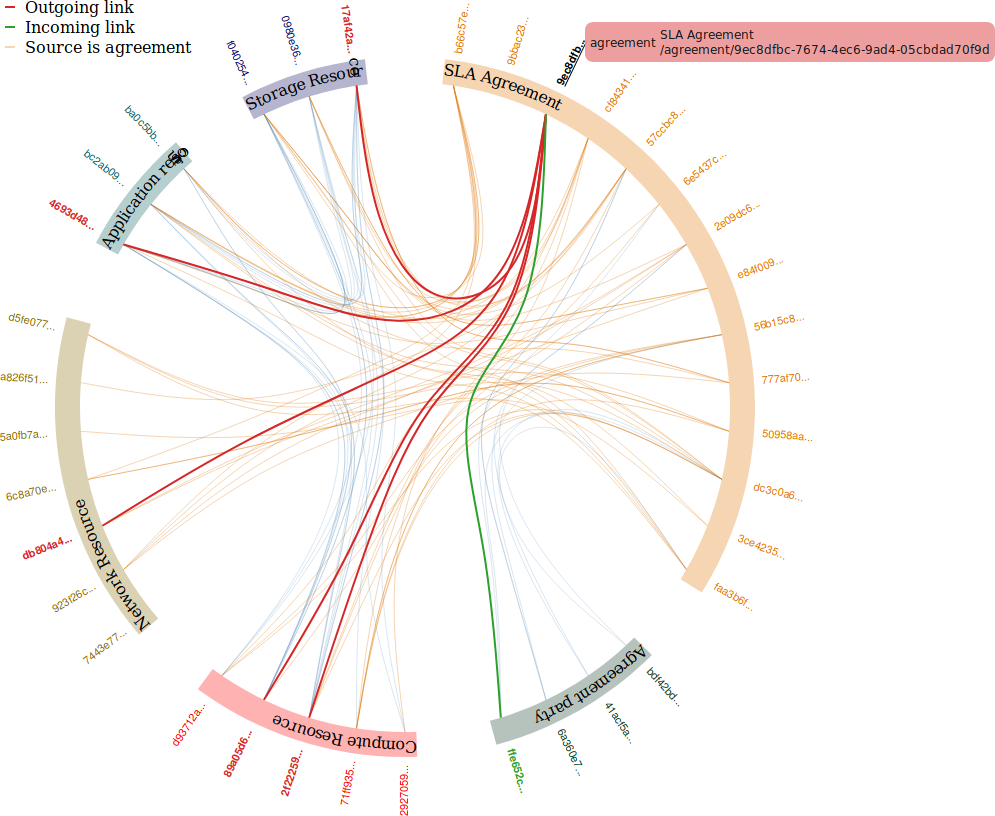
\includegraphics[width=\textwidth]{images/OCCI-relations.png}
		\caption{\emph{OCCI} verknüpft Dienstgüte-Vereinbarungen mit verteilten Anwendungen, Stakeholdern und Cloud-Ressourcen. Die Zuordnung erfolgt Service-bezogen. In der Abbildung ist eine Vereinbarung markiert: Sie wird von einem Anwender beantragt (grüne Linie) und wirkt anschließend auf Ressourcen und darauf aufbauenden Anwendungen (rote Linien). Visualisierung über \emph{OCCIViz}.}
		%		https://github.com/IntelLabsEurope/OCCIViz	
		\label{fig:occi}
	\end{figure}
	
	Auch hier existiert eine experimentelle Implementierung für OpenStack\footnote{\url{https://github.com/openstack/ooi}}. Diese ist jedoch bereits als obsolet gekennzeichnet. Die SLA-Unterstützung ist über ein weiteres Projekt theoretisch verfügbar\footnote{\url{https://github.com/IntelLabsEurope/OCCI-SLAs}}.
	
	\emph{TOSCA} und \emph{OCCI} überschneiden sich nicht: Letzteres dient nicht der Modellierung providerübergreifender Infrastrukturen, sondern ausschließlich der Kommunikation mit der Plattform. Beide Standards ergänzen sich außerdem mit dem \emph{Cloud Data Management Interface (CDMI\footnote{\url{https://www.snia.org/cloud}})} für Verwaltung und Zugriff auf Netzwerkspeicher \cite{snia:2015:cdmi}. Konzeptionell wurden die Standards bereits zu einem modellbasierten Cloud-Orchestrationstool verbunden \cite{korte:2017:toscamp}.
	%Model Driven Cloud Orchestration by Combining TOSCA and OCCI (Position Paper)
	%Fabian Korte, Johannes Martin Erbel, Jens Grabowski
	
	Um sinnvoll nutzbar zu sein, müsste der offene API-Standard von Cloud-Providern implementiert werden. Da dies nicht absehbar ist, bleibt \emph{OCCI} zumindest als interessante Grundlage für die API einer eigenen Cloud-Management-Plattform. Als pragmatischer Ersatz für den Zugriff auf Public-Cloud-Angebote, muss der Einsatz einer Multi-Cloud-Bibliothek evaluiert werden, siehe \autoref{sec:bibliotheken}.		
	
\end{description}

\noindent
Container sind nicht für jede Anwendung einsetzbar. Entsprechend müssen auch klassische virtuelle Maschinen bei einer Multi-Cloud-Migration unterstützt werden. Proprietäre Lösungen sind genauso ungeeignet wie Teillösungen auf einer einzelnen Service-Ebene.

Insgesamt ist der Support für offene Standards im Open-Source-IaaS-Projekt OpenStack am größten. Auf allen Ebenen der Service-Bereitstellung sind zumindest experimentelle Implementierung verfügbar: \emph{cloud-init} zur Imagekonfiguration, \emph{TOSCA} zur Service-Definition und \emph{OCCI} zur Kommunikation mit der Cloud unter Berücksichtigung von SLAs. 

Einige weitere technische Herausforderungen löst ein Multi-Cloud-Broker oder eine CMP: Management von statischen und virtuellen IPs, SSL-Zertifikaten, sowie Load Balancing. Andere Migrationshürden bleiben: Verfügbarkeit von Betriebssystemen, Frameworks und Bibliotheken, ebenso wie die Vereinbarkeit mit vorhandenen Lizenzen. Der folgende Abschnitt gibt eine Übersicht kommerzieller Cloud Management Plattformen sowie bisheriger Forschung zu Inter- und Multi-Cloud-Brokern mit besonderem Blick auf SLAs und Policys. 

\section{Die Limitierungen Kommerzieller CMPs}

Kommerzielle Anbieter wie \emph{RightScale} betonen den Self-Service-Charakter und potentielle Kosteneinsparungen durch ihrer Cloud-Management-Lösungen: Traditionell werden virtuelle Maschinen bei Bedarf von der internen IT bereitgestellt. Dabei entstehen auf der einen Seite Wartezeiten und auf der anderen erhöhter Arbeitsaufwand. 

Eine CMP kann diese Arbeiten automatisieren. Sie helfe laut \emph{Rightscale} die \emph{Schatten-IT} abzubauen -- die entsteht, wenn Mitarbeiter aufgrund langwieriger interner Prozesse zu Public-Cloud-Angeboten greifen -- mit allen negativen Folgen für Sicherheit und Vertraulichkeit. Die automatische Durchsetzung von Policys könnte sich also doppelt lohnen. Nebenbei liefert die CMP einen Preis- und Feature-Überblick der internen und öffentlichen Angebote. So hilft sie das optimale Angebot zu finden.

Nichtsdestotrotz sollte die CMP unabhängig entwickelt und betrieben werden. Cloud-Provider-eigene Lösungen werden daher nicht betrachtet. Weniger geeignet sind auch SaaS-Angebote: Hier entsteht eine neue Abhängigkeit und \emph{Single Point of Failure}. Der nachfolgende Aufzählung zeigt die aktuell verbreitetsten CMP-Lösungen mit besonderem Fokus auf Bereitstellungsmodelle, Funktionsumfang und Offenheit der Schnittstellen.

\todo{(Zusatz) Tabelle}

%Automatisierung oder nur schöne Dashboards?

\begin{description}
	
	\item[Red Hat CloudForms\footnotemark]\footnotetext{\url{https://www.redhat.com/en/technologies/management/cloudforms/}}
	Kommerzielle Cloud Management Platform, Grundlage ist das Open Source-Projekt  ManageIQ\footnotemark\footnotetext{\url{https://manageiq.org/}}, das alle wichtigen IaaS-Provider unterstützt (AWS, Azure, GCP, OpenStack).	
	
	Besonderheit: ein umfangreiches -- optional grafisches -- Policy-Management. Eigene Regeln folgen dem Schema \emph{Bedingung/Ereignis-Aktion}.
	
	Alle Schnittstellen der CMP sind proprietär. Die Orchestrierung liest jedoch vorhandene Vorlagen aus \emph{AWS CloudFormation} and \emph{OpenStack Heat}.
	%http://manageiq.org/docs/reference/latest/doc-Policies_and_Profiles_Guide/miq/
	
	\item[Rightscale CMP\footnotemark]\footnotetext{\url{https://www.rightscale.com/}}
	Proprietäres \emph{Software-as-a-Service}-Angebot, unterstützt alle wichtigen IaaS-Provider, zusätzlich Plattformdienste, Docker-Container und Hypervisoren, besonders \emph{VMware vSphere}.
	
	Infrastruktur und Dienste werden als Vorlagen in einem eigenen Katalog bereitgestellt. Dabei erlaubt Rightscale auch heterogene Anwendungen über IaaS-, CaaS- und PaaS-Grenzen hinweg.
	
	Ein Dashboard zeigt Empfehlungen zur Kostenoptimierung, allerdings ohne SLAs einzubeziehen.
	
	\item[Scalr] 
	
	%	Whitepaper! 
	
	\item[Cloudify\footnotemark]\footnotetext{\url{https://cloudify.co/}} implementiert den \emph{TOSCA}-Standard und ist in einer Open-Source-Version erhältlich. Mithilfe (grafischer) Werkzeuge lassen sich Cloud-Infrastrukturen und Services modellieren. Plugins erweitern Cloudify um wichtige Provider; sowohl auf IaaS- (AWS, Azure, GCP, OpenStack) als auch auf CaaS-Ebene (Kubernetes). Konfiguration wie das Start-Skript kann direkt übergeben, oder über ein Tool wie Puppet weitergeleitet werden. 
	
	Einfache Policys sind integriert, mithilfe eines rudimentären Monitorings und der Provider-Plugins werden diese umgesetzt. Der (grafische) TOSCA-Editor und echtes Cluster-Management sind allerdings nur in der proprietären Enterprise-Ausgabe enthalten.


\end{description}

% https://www.embotics.com/solutions-cloud-governance
% Nur Azure und Amazon. Cloud Governance: Die richtigen Meta-Tags zu Instanzen hinzufügen. Kostenoptimierungsvorschläge, aber nur die Wahl zwischen zwei Providern.




%DivvyCloud (Commercial) 
%
%Automation Bots to schedule downtime, terminate, or re-size instances and resources so you only pay for what you use 
%
%https://divvycloud.com/product/botfactory/for-cost/ 

%
%Commercial Tools 
%
%https://www.cloudyn.com/ 
%
%close-source 
%
%only cost monitoring and optimization 
%
%Also, Rightscale, Cloudhealth, CloudCheckr 


%Apache Scalr (complex, freemium) 

\section{Bisherige Forschungsarbeiten}

% Multi-Cloud Übersichtspaper: Umfagreichste Cloud-Hierarchie Betrachtung! Einleitung, Produkte, Herausforderungen
%the  security  breaks  have  brought
%into discussions the trustfulness of the Hybrid Cloud.
%A  solution  to  a
%recommendation  system
%is  therefore
%needed in Multi-Cloud, and very few prototypes are
%currently available as the trust management problem
%is more than a technical one.
%Consuming Resources and Services from Multiple Clouds
%From Terminology to Cloudware Support
%Dana Petcu

Besonders interessant sind bisherige Arbeiten, die neben einer Föderation auch Hybrid- oder Multi-Cloud-Brokering unterstützen. Es sollten also keine Cloud-internen Plugins oder Agenten nötig sein.

Die folgende Übersicht geht besonders auf den Umfang der Policy- und SLA-Fähigkeiten ein: Diese sollten nicht nur während des Brokerings beachtet werden, sondern kontinuierlich zur Laufzeit. Auch die Einhaltung von Standards zu Service- und Ziel-Definitionen, sowie Kommunikation sind relevant. Unterschiede gibt es bei der Art unterstützter Anwendungen; neben Stapelverarbeitungsjobs und High-Performance-Computing sollten auch reguläre, interaktive Web-Anwendungen verwaltet werden können. 

Auch nicht-funktionale Anforderungen werden betrachtet: Sind die Artefakte der Projekte noch als Code verfügbar oder sogar in Open-Source-Tools und kommerziellen Produkten aufgegangen?

%policy-driven service placement optimization in federated clouds 


\begin{description}	
	
	
	\item[InterCloud] ist ursprünglich eine Föderation von Cloud-Ressourcen \cite{buyya:2010:intercloud}. Auf einem zentralen Marktplatz \emph{zeigen} Clouds ihre Dienste, oder \emph{kaufen} sie je nach Bedarf. Für diese aktive Teilnahme sind Cloud-interne Agenten nötig.
	
	Vorgeschlagen werden zusätzlich externe Adapter, über die einerseits Provider \emph{unfreiwillig} in die Föderation integriert werden, andererseits aber auch weitere Teilnehmer Ressourcen kaufen können. Hierüber könnten auch Anwendungsbroker die Ressourcen der Föderation nutzen.
	
	Der Ansatz fokussiert sich stark auf das Preis-gesteuerte Brokering, beachtet optional aber auch Geostandorte. Die Provider unterstützen eingeschränkt SLAs. Verteilt werden nur Rechenaufgaben, interaktive Anwendungen sind nicht vorgesehen.
	%	5, 37, 38 Grozev
	
	
	\item[Contrail] ist eine zentral gemanagte Föderation \cite{carlini:2011:contrail}. SLAs gelten für den gesamten Cloudverband, nicht für einzelne Anwendungen. Das zentrale Element, der \emph{Federation Runtime Manager}, verteilt jedoch individuelle Nutzeranfragen und beachtet dabei Preis und Leistung.
	
%	http://contrail-project.eu/architecture

	Contrail versteht sich als PaaS und unterstützt auch Hadoop. Ähnlich zu InterCloud sprechen externe Adapter theoretisch weitere Provider an, die sich der Föderation nicht bewusst sind.
		
	
	\item[RESERVOIR] entwickelt eine Peer-to-Peer-Föderation mit eigenen Service-Schemata und Inter-Cloud-Protokollen \cite{rochwerger:2009:reservoir}. Ein Unterprojekt abstrahiert die Cloud-Ressourcen durch eine zusätzliche Schicht, sodass Java-Anwendungen transparent auf allen Providern ausgeführt und migriert werden können \cite{rochwerger:2011:reservoir-multi-cloud}. Ein Broker beobachtet Performance-SLAs und skaliert die Instanzen entsprechend.
%	IBM, Telefonica, SAP + Universites, EU-funded
	
	
	\item[Optimis] baut auf eine zentrale \emph{Deployment Engine (DE)} \cite{ferrer:2012:optimis}. Über interne und externe Adapter verbinden sich Cloud-Provider und senden ihre Ressourcen-Angebote. Soll eine Anwendung ausgerollt werden, wählt die DE passende Provider aus und sendet ihnen ein SLA-Template. Diese antworten mit einer Zusage, Absage oder einem Gegenvorschlag. Aus allen Antworten wählt der DE anschließend das beste Angebot. Dabei beachtet sie quantitative Größen wie den Preis, aber auch Erfahrungswerte wie Zuverlässigkeit oder die Energieeffizienz eines Providers.
	
	Die internen Adapter vertreten Föderationsmitglieder -- sie lehnen eine Anfrage des DE ab, wenn sie für den Cloud-Provider finanziell unattraktiv ist. Eine weitere Komponente, der \emph{Service Optimizer}, beobachtet alle Anwendungen auf SLA-Verletzungen. Wie genau SLAs spezifiziert werden können ist nicht deutlich. Auch der Matching-Algorithmus ist nicht öffentlich. Geostandorte werden nicht beachtet. Externe Adapter sind rein konzeptionell und nicht implementiert.
	
	Die Arbeit geht auch auf die Bereitstellung von Laufzeitumgebungen und Provider-spezifischen Images ein: Er schlägt eine Erweiterung des \emph{Open Virtualization Formats (OVF)} vor. Zusätzliche Metadaten beschreiben die nötige Cloud-Konfiguration.
	
	
	\item[Bernsetein InterCloud Blueprint] Eine weltweite Föderation der Cloud-Ressourcen \cite{bernstein:2011:intercloud}. Interessant ist der dezentrale Ansatz des Brokerings. Nur in dieser Arbeit wird der Broker als \emph{Single Point of Failure} erkannt: deshalb soll er zwangsläufig repliziert und in allen Regionen mindestens einmal verfügbar sein. Der Ansatz folgt also den Grundlagen des Internets und entwickelt eigene Inter-CLoud-Protokolle auf Basis von XMPP und RDF.
	
	
	\item[STRATOS] ist eine Cloud-Management-Plattform mit integriertem Multi-Cloud-Broker \cite{pawluk:2012:stratos}. Anwendungen werden über das eigenentwickelte, XML-basierte \emph{Topology Descriptor File (TDF)} beschrieben. Es enthält die Service-Architektur und zusätzlich Policys und SLOs. Für den Zugriff auf externe Clouds existiert ein \emph{Translation Layer}, der eine einheitliche API bereitstellt. Die Arbeit fokussiert sich auf die Bereitstellung klassischer Web-Anwendungen und Kostenoptimierung. Der mittlerweile nicht mehr weiterentwickelte \emph{Service Measurement Index (SMI)} definiert die Ziele.
%	https://www.google.de/url?sa=t&rct=j&q=&esrc=s&source=web&cd=1&ved=0ahUKEwju27vHs6DZAhUCWRQKHRv7BEcQFggrMAA&url=http%3A%2F%2Fwww.mikesmit.com%2Fwp-content%2Fpapercite-data%2Fpdf%2Fcloud2012.pdf&usg=AOvVaw3e6yhHYmhWBbIxtr7MqkuX
	
	\item[Meryn] ist eines der wenigen Implementierung eines SLA-bezogenen PaaS-Systems \cite{dib:2013:meryn}. Aktuelle Plattformen begrenzen hauptsächlich den Ressourcenverbrauch der Gastanwendungen -- Meryn schlägt zusätzlich eine Kostenoptimierung für Provider vor.
	
	Cloud-interne \emph{Cluster-Manager} bieten in einem Wettbewerb um Ausführungsaufträge. Die Arbeit fokussiert sich auf Stapelverarbeitung mit Hadoop und anderen Framworks. Dabei entwickeln die Autoren für jedes Framework eine eigene VM, die jeweils einmal pro Cluster ausgeführt wird. Vorgestellt wird außerdem ein \emph{Cloud-Bursting-Ansatz}, bei dem zusätzliche Ressourcen in Public Clouds angemietet werden.
	
	
	\item[SeaClouds] ist ein EU-finanziertes PaaS-Management-Projekt mit großem Umfang \cite{seaclouds:2015:architecture}. Vorgeschlagen wir ein Referenzmodell aus \emph{Planner}, \emph{Deployer}, \emph{SLA Service} und \emph{Monitor}. Hierüber lassen sich verteilte Anwendungen modellieren, auf verschiedenen Providern bereitstellen und SLA-bezogen verwalten.
	
	Besonderheit ist die Unterstützung von offenen Standards wie der \emph{Cloud Application Management for Platforms} für APIs und TOSCA zur Service-Modellierung. Angebote der Cloud-Provider werden kontinuierlich überwacht und als \emph{TOSCA}-Graph abgebildet. SLAs nutzen allerdings nicht \emph{TOSCA}, sondern \emph{WS-Agreements}.
%	http://wsag4j.sourceforge.net/site/wsag/wsag-language.html
		
	Erwähnt wird eine Provider-unabhängige Lösung, konkret umgesetzt ist dies jedoch nur für die Open-Source-PaaS-Projekte \emph{OpenShift} und \emph{CloudFoundry}.
	
	\item[TOSCAMP] oder \emph{End-to-End Orchestration of
	Multi-Cloud Applications}, kombiniert in einem Prototypen die Standards \emph{TOSCA} und \emph{CAMP} \cite{korte:2017:toscamp}. Eine verteilte Anwendung wird abstrakt als \emph{TOSCA}-Template inklusive einfacher Policys beschrieben. Anschließend wandelt \emph{TOSCAMP} diese Beschreibung in einen \emph{CAMP}-Plan zur Multi-Cloud-Installation.

	Im Gegensatz zu anderen Cloud-Management-Plattformen erstellt \emph{TOSCAMP} keinen internen Graph einer Anwendung -- stattdessen erweitert die Arbeit \emph{CAMP} um Policys und bildet alle Installationen in einer YAML-Datei ab. Einen ähnlichen Ansatz verfolgt das Projekt \emph{brooklyn-tosca\footnote{\url{https://github.com/cloudsoft/brooklyn-tosca}}}.
	
%	\item[An SLA-based Broker for Cloud Infrastructures] Nicht nur Private Clouds sondern auch Personal Devices 
%	
%	Modulare Architektur 
%	
%	wechselnde und unzuverlässige Provider
%	
%	Fokus auf Föderation. Aber: Idee der forced integration of commercial cloud providers 
	
\end{description}

%Mist.io Open source 
%Build on libcloud and cloudify
%Can monitor costs (commercial)
%No automatic scheduling 

\noindent
Im Gegensatz zu den kommerziellen Projekten liegt der Fokus vieler Forschungsarbeiten auf Cloud-Föderationen und SLA-basiertem Brokering. Einige unterstützen über Adapter konzeptionell mehrere Bereitstellungsmodelle; je nachdem, ob dem Cloud-Provider die Mitgliedschaft in einer Föderation bewusst ist. Interne Adapter sprechen mit zusätzlichen, Cloud-internen Erweiterungen. Externe Adapter nutzen die öffentlichen APIs von Drittanbieter-Clouds. Hier entsteht zwar Mehraufwand, dieser könnte in weiteren Entwicklungen jedoch von einer Multi-Cloud-Bibliothek gemildert werden.

Negativ fällt auf, dass die Artefakte der meisten (EU-)Forschungsprojekte
nicht mehr verfügbar sind. Auch Matching-Algorithmen sind teilweise nicht veröffentlicht. Die Ergebnisse lassen sich so nicht mehr nachvollziehen. Ohnehin basieren sie oft auf veralteten Technologien: Formate wie \emph{OVF} werden in modernen IaaS-Plattformen nicht mehr unterstützt. Demgegenüber spielen Container oder Serverless-Computing keine Rolle.

Wie bereits beschrieben, existieren eine Vielzahl von offenen Cloud-Standards. Von Service-Definition über SLAs bis zur standardisierten Kommunikation mit der Management Plattform. In der Forschung werden diese aber nur selten aufgegriffen und stattdessen neu erfunden. Besonders deutlich wird die in einer Forschungsübersicht der Europäischen Kommission.
%Cloud Computing Service Level
%Agreements
%Exploitation of Research Results
%Editor: Dimosthenis Kyriazis
Das eigentliche Problem der Portabilität im Cloud-Umfeld lässt sich so nicht lösen.

Insgesamt bleibt vor allem die unterschiedliche Ausrichtung von Forschungsprojekten und kommerziellen Anbietern: Forschungsprojekte fokussieren sich auf Föderationen. Dies entspricht auch dem vorherrschenden Cloud-Typ innerhalb der verantwortlichen Organisationen. SLAs werden ausschließlich von diesen ausgewertet und teilweise umgesetzt. Kommerzielle Projekte sind dagegen meist externe Broker, stellen Preisunterschiede und Kosten dar. Statt SLAs beachten sie nur einfache Policys.

Das folgende Kapitel erstellt aus den bisherigen Überlegungen zu Anforderungen, Schemata und Forschungsergebnissen einen Vorschlag für SLA-basiertes Brokering auf Basis moderner Technologien.

	\chapter{Entwurf und Implementierung}
\label{cha:implementierung}

\todo{Kapitel-Einleitung}



\section{Modularer Architektur-Vorschlag}

%Komponenten des Brokers.
%
%
%In der CMP: Polling oder Notification?
%
%Was löst eine Aktion aus?
%- Monitoring der Services
%- Änderung der Umgebung
%- User-Aktion
%- Ergebnis einer anderen Policy

\begin{figure}
	\centering
	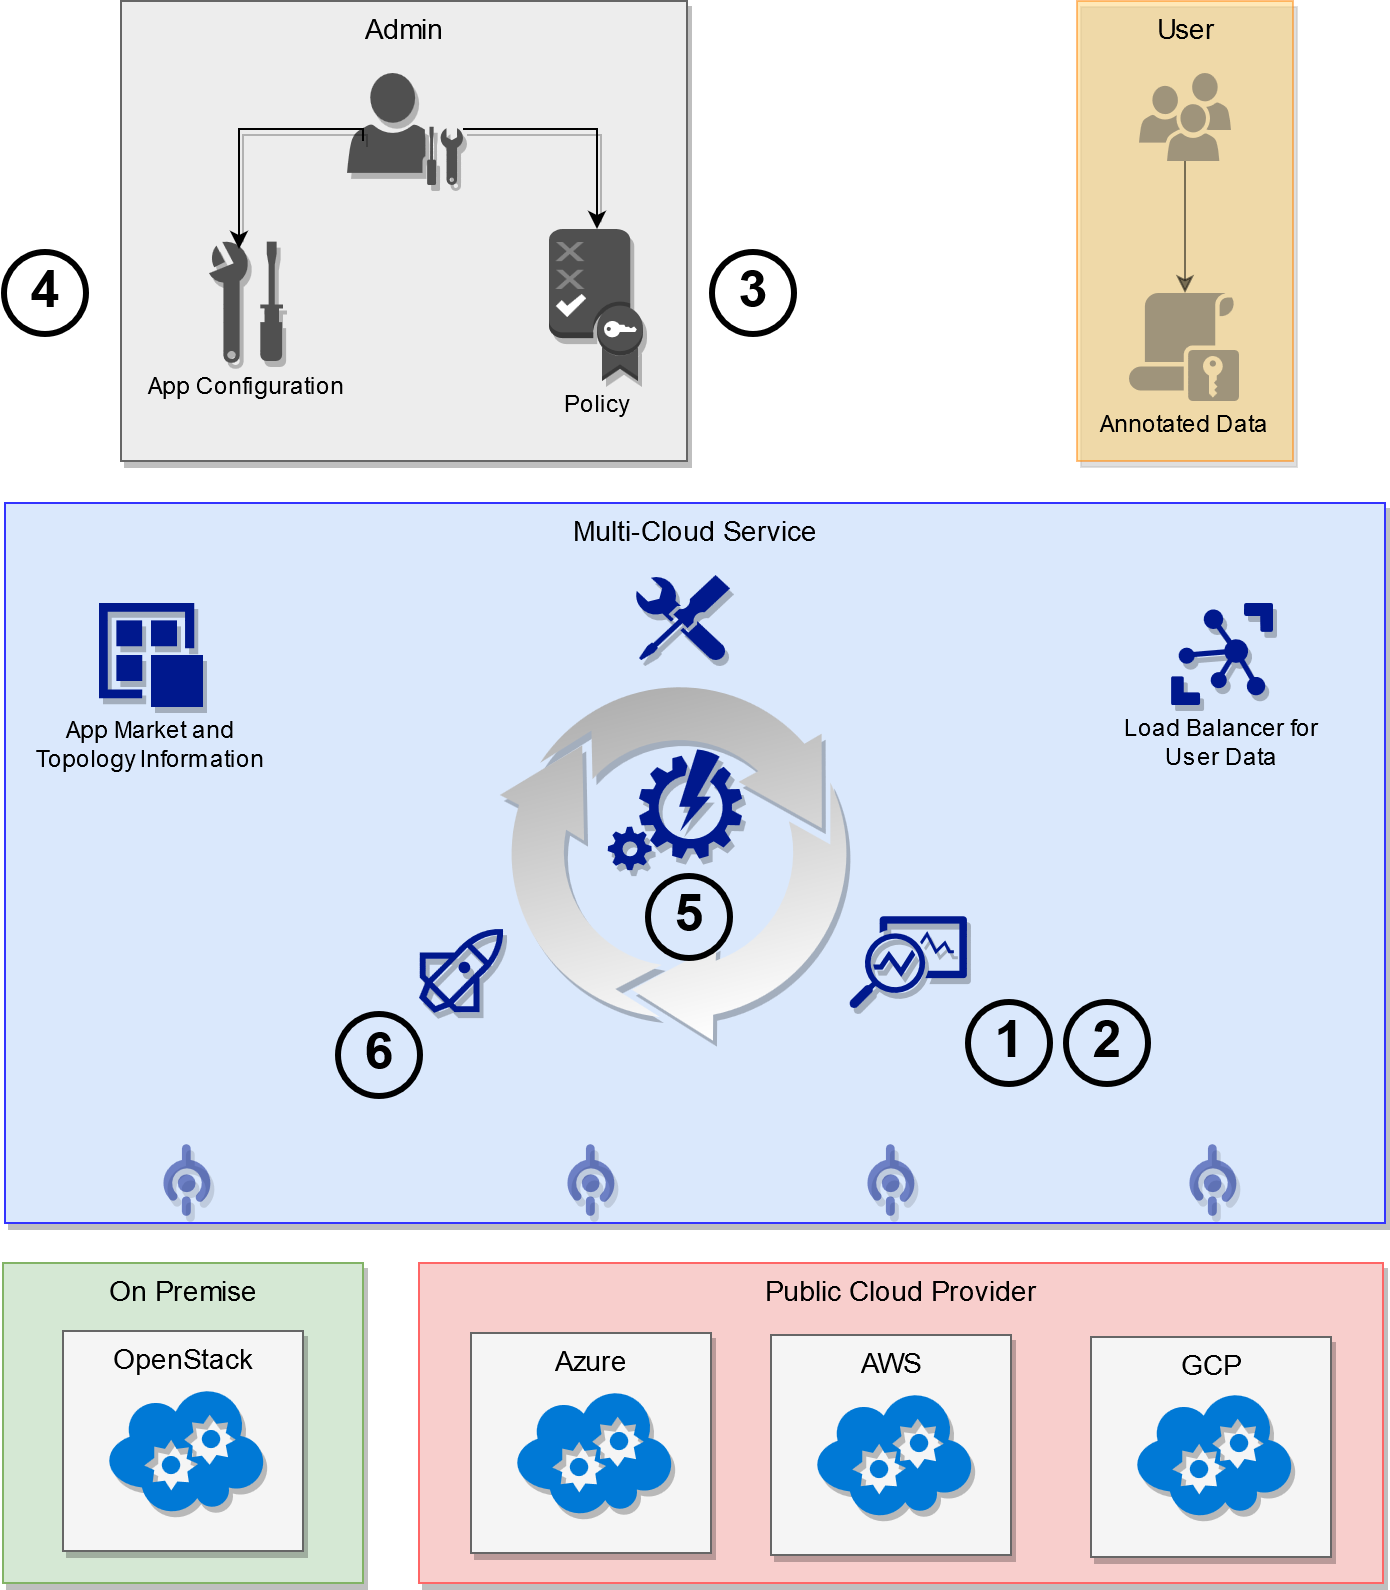
\includegraphics[width=0.9\linewidth]{images/cycle}
	\caption{}
	\label{fig:cycle}
\end{figure}

%Zyklus\autoref{fig:cycle}:

%\begin{description}
%	\item[Nummerierte Aufzählung]~\par
\begin{enumerate}
	
	\item Sammeln der Meta-Informationen alle Cloud-Provider
	\begin{enumerate}
		\item Kapazität (CPU, RAM, HDD, Network)
		\item Features (Verschlüsselung, CUDA, …)
		\item Geo-Lokation 
		\item Preis
	\end{enumerate}
	
	\item Sammeln der Laufzeitinformationen der PaaS/Anwendungen
	\begin{enumerate}
		\item Auslastung
		\item Fehler
		\item Ausfälle
	\end{enumerate}
	
	\item Sammeln der SLAs
	\begin{enumerate}
		\item Policy-Definitionen
		\item Policy-Konfiguration
		\item Placement-Algorithmen
	\end{enumerate}
	
	\item Neue Anwendung/Änderung eines SLA
	
	\item Optimierung
	\begin{enumerate}
		\item Feste Vorgaben (Geo, Backup)
		\item Weiche (Preis, Latenz, Verfügbarkeit)
	\end{enumerate}
	
	
	\item Ausführung
	\begin{enumerate}
		\item Netzwerkkonfiguration
		\item Allokation/De-Allokation von Ressourcen
		\item Deployment
		\item Migration
		\item Logging/Benachrichtigung
		\item Backup
	\end{enumerate}
	
\end{enumerate}

\section{Brokering}


%https://de.wikipedia.org/wiki/Constraintprogrammierung
%https://de.wikipedia.org/wiki/Scheduling

%entailing multiple constraint satisfaction (MCS)
%
%\todo{Schaubild, was wird wann gematcht}
%% Pseudocode des Algorithmus, wie in Meryn
%
%Kostenoptimierung
%
%Preisentwicklung? 
%
%Migration je nach Tageszeit? 
%
%Kosten der Datentransfers 
%
%Subscription On-Demand/Monthly/Yearly 
%
%Kompliziert durch undurchsichtige Staffelpreise
% https://www.rightscale.com/blog/cloud-cost-analysis/aws-vs-azure-vs-google-cloud-pricing-compute-instances

%https://www.rightscale.com/blog/cloud-cost-analysis/comparing-cloud-instance-pricing-aws-vs-azure-vs-google-vs-ibm

%
%Cost Calculators 
%
%http://go.appscale.com/cloud-cost-calculator-help 
%
%https://github.com/ifosch/accloudtant 
%
%https://awstcocalculator.com/# 
%

\section{Testumgebung: OpenStack \& Hyrise-R}

Hyrise\footnote{\url{https://hpi.de/plattner/projects/hyrise.html}} ist eine In-Memory-Forschungsdatenbank der Fachgruppe \emph{Enterprise Platform and Integration Concepts (EPIC)} am Hasso-Plattner-Institut \cite{grund:2010:hyrise}. Die Datenbank teilt sich einige Eigenschaften mit \emph{SAP HANA}\footnote{\url{https://www.sap.com/products/hana.html}}: Ein \emph{Delta Store}, spaltenorientierte Speicherung, Wörterbuchkodierung und weitere Komprimierungstechniken sowie den \emph{Insert-Only}-Ansatz und Partitionierung. Herausragend ist die OLAP-Performance, enthalten sind aber auch Optimierungen für OLTP-Aufgaben.

Hyrise-R ist eine Erweiterung des Basisprojektes um Replikation \cite{schwalb:2015:hyrise-r}. Es folgt dabei dem \emph{Scale-Out}-Ansatz: Alle schreibenden Operationen werden auf einem einzigen \emph{Master-Node} durchgeführt. Dessen Datensatz wird in weniger als einer Sekunde (\emph{lazy}) mit beliebig vielen \emph{Replica-Nodes} abgeglichen. Diese Spiegelungen bearbeiten alle reinen Leseanfragen und machen den Verbund so skalierbar, siehe \autoref{fig:hyrise-r}. Nach dem \emph{CAP-Theorem} sind Verfügbarkeit und Partitionstoleranz hier also wichtiger als Konsistenz. 

	\begin{figure}[ht]
	\centering
	\def\svgwidth{\textwidth}
	\includesvg{images/hyrise-r}
	\caption{Verteilte \emph{Hyrise-R}-Architektur mit getrennter Verarbeitung von Lese- und Schreibanfragen. Der Master-Knoten dient als \emph{Single Source of Truth}. Zur Leistungssteigerung übernehmen Spiegelserver die Beantwortung der meisten Leseanfragen. Kleinere Inkonsistenzen werden dabei in Kauf genommen. Aus \cite{ssiclops:d42:experiments-measurements}.}	
	\label{fig:hyrise-r}
\end{figure}

Durch die verteilte Architektur ist Hyrise-R ein potenzieller Kandidat als Testanwendung innerhalb der Multi-Cloud-Umgebung. Einige \emph{SSICLOPS}-Teilprojekte untersuchten bereits Zuverlässigkeit, Performance, Datensicherheit und Vertraulichkeit in einer privaten OpenStack-Föderation \cite{ssiclops:d23:security-extensions, ssiclops:d42:experiments-measurements, bastian:2017:openstack-policies}. \todo{Diagramm:Hyrise-R on SSICLOPS}

Im Rahmen dieser Arbeiten sind einige Infrastrukturteile als Code veröffentlicht: So existiert zum Beispiel eine Docker-Teststellung mit grafischem Cluster-Manager, um die Performance bei verschiedenen Replikationsstufen zu prüfen. Diese Infrastruktur wurde in mehreren Studienarbeiten weiter angepasst, um Hyrise-R-KVM-Images in OpenStack bereitzustellen \cite{eschrig:2016:ssiclops-masterproject, maschler:2017:ssiclops-masterproject}. Möglicherweise können Teile dieser Arbeiten weiterentwickelt werden.


\section{Multi-Cloud-Bibliotheken}
\label{sec:bibliotheken}
\todo{Kleines Architektur Diagramm}

Ziel ist die Implementierung eines externen Broker-Services oder die Aufwertung einer verteilten Anwendung für den automatischen Betrieb in mehreren Clouds. Da unabhängige Cloud-Provider keine einheitlichen APIs anbieten, stellt dieses Kapitel verschiedene Bibliotheken vor, um möglichst viel der zusätzlichen Komplexität zu verbergen.

Ohne weitere Bibliotheken müsste für jede zu berücksichtigende Cloud das jeweilige SDK eingebunden werden. Auch Namensgebung, Architektur und Prozesse unterscheiden sich von Anbieter zu Anbieter. \todo{Mention Standard Cloud API OASIS TOSCA}

Durch den Einsatz einer Drittbibliothek ergibt sich allerdings eine potenzielle Schwachstelle. Falls diese fehlerhaft ist oder gar nicht weiter entwickelt wird, gefährdet dies das ganze Projekt. Historie und Zukunftschancen spielen bei der Auswahl eine zentrale Rolle. Im Optimalfall abstrahiert die Bibliothek Änderungen der Provider-SDKs. Ob und wie groß die Arbeitserleichterung ausfällt, prüft der Praxisteil.

Im Folgenden untersuchen wir die Eignung der populärsten Bibliotheken. Wichtigste Komponente ist dabei das Computing-Modul. Wünschenswert wäre auch Container-Unterstützung, um Images anbieterunabhängig bereitzustellen. Gestartete Anwendungskomponenten erfordern für die erste Erreichbarkeit oft Zugriff auf die DNS-Einstellungen der Cloud. Optional ist die Unterstützung von \emph{Content Delivery Networks}, Speicher- und Backup-Diensten.

% https://tex.stackexchange.com/questions/341592/hyphenating-text-inside-tabularx
\begin{table*}\centering
	\begin{minipage}{\textwidth}
	\caption{Übersicht freier Multi-Cloud-Bibliotheken. Mit $*$ gekennzeichnete Eigenschaften sind experimentell. Aufgeführt sind nur die populärsten Cloud-Provider, die Bibliotheken können darüber hinaus weitere unterstützen. Ob eine Bibliothek weitere Informationen, wie aktuelle Preisinformationen und den Standort des Rechenzentrums abrufen kann, zeigt die Spalte \emph{Cost\,/\,Geo}.}
	\ra{1.3}
	\begin{tabularx}{\textwidth}{>{\centering}XXXr} \toprule
		Projekt & Cloud-Provider & Cloud-Services & Cost\,/\,Geo\\ \midrule
		Apache Libcloud (Python)\footnotemark & AWS, Azure, OpenStack, GCP, Docker & Compute, Container, DNS, Load Balancer, Storage, Backup & $x$\,/\,$x$\\
		Apache jclouds (Java)\footnotemark & AWS, Azure, Open\-Stack$*$, GCP, Docker & Compute, Container, Load Balancer$*$, Storage & $x$\,/\,$x$\\
		PkgCloud (Node.js)\footnotemark & AWS, Azure, OpenStack& Compute, Load Balancer, Storage$*$, DNS$*$ & --\,/\,--\\
		Libretto (Go)\footnotemark & AWS, Azure, OpenStack, GCP & Compute & --\,/\,--\\
		Fog (Ruby)\footnotemark & AWS, OpenStack, GCP & Compute, DNS, Storage & $x*$\,/\,--\\
		\bottomrule
	\end{tabularx}
	\label{tab:bibliotheken}
	\vspace{150pt}
	\footnotetext[1]{\url{https://libcloud.apache.org/}}
	\footnotetext[2]{\url{https://jclouds.apache.org/}}
	\footnotetext[3]{\url{https://github.com/pkgcloud/pkgcloud/}}
	\footnotetext[4]{\url{https://github.com/apcera/libretto/}}
	\footnotetext[5]{\url{http://fog.io/}}
\end{minipage}  
\end{table*}

\autoref*{tab:bibliotheken} listet die untersuchten Bibliotheken mit unterstützten Cloud-Providern, Services und weiteren Features. Letzteres sind Zugriff auf Preisinformationen des Anbieters und Standortinformationen der Rechenzentren. Zusätzlich sollten die Projekte kontinuierlich weiterentwickelt werden, eine aktive Entwicklergemeinschaft besitzen und gut dokumentiert sein. Alle sind Open Source und unter einer freien Lizenz verfügbar.

\begin{description}
	
	\item[Apache jclouds] existiert schon seit 2009. Es unterstützt zumindest experimentell die wichtigsten Provider, aber nicht alle Services: DNS ist nicht vorhanden, Container-Unterstützung gibt es nur für Docker. Die Bibliothek ist gut getestet, dokumentiert, und mit zahlreichen Beispielen ausgestattet. Durch Java ist sie außerdem typsicher. 
	
	\emph{jclouds} ist außerdem Grundlage mehrerer Multi-Cloud-Projekte, z.\,B. von \emph{Apache brooklyn\footnote{\url{https://brooklyn.apache.org/}}}: Mithilfe von \emph{CAMP}-Plänen lassen sich Anwendungen über mehrere Clouds ausrollen.

	\item[Apache Libcloud] vereint viele Vorteile: Es unterstützt neben OpenStack, als Referenz für Private-Cloud-Installationen, alle großen und kleinen Cloud-Provider mit allen Kernservices. Besonders interessant ist der Container-Support für \emph{Docker}, \emph{Kubernetes}, \emph{Amazon ECS} und die \emph{Google Container Engine}. Entsprechend gepackte Anwendungen könnten in einer Vielzahl von Clouds ohne weitere Änderungen ausgeführt werden.

	\item[Fog] integriert die wichtigsten Anbieter und Services. Die Entwicklergemeinde rund um \emph{Fog} ist aktiv und die Bibliothek wird häufig eingesetzt. Besonders interessant sind die bereitgestellten Mocks, die Tests des neuen Services erleichtern sollen. Zumindest für OpenStack wird Metering unterstützt. Eine einheitliche Namensgebung der verschiedenen Cloud-Produkte existiert nicht.

	\item[Libretto] beschränkt sich ausdrücklich auf die Compute-Funktionalität mithilfe virtueller Maschinen. Das zugehörige Projekt ist aktiv, kommt aufgrund der fehlenden Funktionalität aber nicht infrage.

	\item[PkgCloud] ist die einzige bekannte \emph{Node.js}-Bibliothek. Funktionsumfang und einheitliche Namensgebung der Cloud-Services sind überzeugend; leider wird die Bibliothek seit dem Verkauf des federführenden Unternehmens nicht mehr aktiv gepflegt. Bereits eingereichte Pull Requests werden nicht bearbeitet. Damit scheidet \emph{PkgCloud} für das Projekt aus.

\end{description}

\noindent Vielversprechend war außerdem das \emph{Apache DeltaCloud}-Projekt: Aufbauend auf \emph{Ruby} stellt es nicht nur eine einheitliche API nach \emph{Cloud Infrastructure Management Interface}-Standard\footnote{\url{https://www.dmtf.org/standards/cloud}} für die Kernfunktionen der wichtigsten Cloud-Provider, sondern auch zusätzliche Client-Bibliotheken und Mock-Funktionen. Aufgrund des plötzlichen Rückzugs von \emph{Red Hat} erfolgt seit 2013 allerdings keine Weiterentwicklung mehr \cite{androu:2013:deltacloud-red-hat-end}. Dieses Beispiel zeigt die Wichtigkeit nicht-funktionaler Betrachtungen bei der Auswahl einer Bibliothek. Auch Apache-Top-Level-Projekte haben nicht unbedingt eine sichere, vorhersagbare Zukunft.

Darüber hinaus existieren spezialisierte Bibliotheken wie \emph{SimpleCloud}\footnote{\url{https://framework.zend.com/manual/1.11/de/zend.cloud.html}} auf \emph{PHP}-Basis, das allerdings eine feste Komponente im \emph{Zend Framework} ist. Auch gibt es neue Entwicklungen wie \emph{CloudBridge}\footnote{\url{https://github.com/gvlproject/cloudbridge}} auf \emph{Python}-Basis. Besonderheit hier: Die Abstraktionsschicht nutzt die nativen SDKs der Cloud-Provider. \emph{CloudBridge} ist leider noch in einem frühen Entwicklungsstadium und als experimentell gekennzeichnet.

\emph{Libcloud} fasst die verschiedenen Cloud-Angebote nicht nur in gemeinsamen Namensräumen zusammen, sondern normalisiert auch Leistungsklassen. Python erleichtert außerdem den Einstieg und fügt sich in viele \emph{Python}-basierte Systemautomatisierungen ein. Diese Multi-Cloud-Bibliothek wird also im weiteren Verlauf der Arbeit erprobt.

%https://brooklyn.apache.org/learnmore/theory.html
% Apache Brooklyn hat eine eigene YAML-Service-Description-Spezifikation, ähnlich zu CAMP, der Clou Application Management API. Die Integration von TOSCA ist geplant, und in einer anderen Arbeit bereit umgesetzt: 
%Trans-Cloud: CAMP/TOSCA-based Bidimensional Cross-Cloud
% Keine SLAs, sondern nur Trigger-Action-Policies.
% Nutzt intern jclouds zur Provider-Anbindung.

\section{OpenStack-Testbed}

Als Beispiel für eine Private-Cloud -- als Teil unseres Multi-Cloud-Setups -- soll OpenStack dienen. Es ist das populärste Open-Source-Projekt um eigene Infrastruktur als Service aufzubauen. Gesponsert wird es von Großunternehmen wie \emph{HPE}, \emph{IBM}, \emph{Canonical}, \emph{Red Hat} und anderen.

OpenStack setzt sich aus verschiedenen Teilprojekten zusammen, die jeweils einen Dienst entwickeln und bereitstellen. Ein Minimal-Setup besteht aus \emph{Nova} (Computing), \emph{Key\-stone} (Authentifizierung), \emph{Neutron} (Netzwerk) und \emph{Glance} (Images). Verbreitet sind außerdem \emph{Cinder} (Blockspeicher) und \emph{Horizon} (Dash\-board). Diese sollen auch in unserem Beispiel genutzt werden. Denkbar ist darüber hinaus die Integration eines Container-Dienstes. Der Zugriff auf die Infrastruktur erfolgt entweder über das Dashboard, Kommandozeilentools oder eine REST-API.

Grundsätzlich wäre auch der Aufbau einer OpenStack-Föderation wie in \emph{SSICLOPS} denkbar \cite{ssiclops:2015:d6.1-project-presentation}. Föderierte Cloud-Architekturen teilen sich zentrale Komponenten, in OpenStack mindestens den Authentifizierungsservice \emph{Keystone}. Je nach Föderationsvariante (\emph{Cells}, \emph{Regions}, \emph{Availability Zones} oder \emph{Host Aggregates}) sind auch Dienste wie Dashboard oder Speicher nur einmal vorhanden. Diese Architektur reduziert Fixkosten, erfordert allerdings spezielle Anpassungen innerhalb der Cloud. Auch gehen einige Vorteile wie Ausfallsicherheit und Unabhängigkeit der zentralen Dienste wieder verloren. Eine Kombination mit weiteren Cloud-Providern im Rahmen unseres Multi-Cloud-Setups ist denkbar, bleibt aufgrund der aufwendigen Einrichtung aber außen vor. Auch wäre der zusätzliche Erkenntnisgewinn vermutlich gering.\todo{SSICLOPS-OS-Architektur}

Selbst ein minimales OpenStack-Testsetup ist durch die diversen Dienste komplex. Denkbar wäre also auch die Nutzung von externen OpenStack-Angeboten. In diesem Projekt gibt es hierfür grundsätzlich drei mögliche Bereitstellungsmodelle: 

\begin{enumerate}
	\item Public Cloud
	\\\emph{Betrieb auf geteilter Cloud-Infrastruktur}
	
	\item Hosted Private Cloud
	\\\emph{Betrieb auf exklusiver Cloud-Infrastruktur}
	
	\item Lokale Testinstallation
	\\\emph{Betrieb auf eigener physischer oder virtueller Infrastruktur}
\end{enumerate}

\noindent Eine Liste öffentlicher OpenStack-Angebote findet sich auf der Projekthomepage\footnote{\url{https://www.openstack.org/marketplace/hosted-private-clouds/}}. Dort werden auch weitere Informationen wie Funktionsumfang und Zertifizierungen aufgeführt. 

Interessant ist zum Beispiel das Angebot der Deutschen Telekom \emph{Open Telekom Cloud\footnote{\url{https://cloud.telekom.de/en/infrastructure/open-telekom-cloud/}}}: eine Public Cloud auf OpenStack-Basis -- in Deutschland -- mit vollem Funktionsumfang und API-Zugriff. International bietet \emph{Rackspace} eine Hosted Private Cloud\footnote{\url{https://www.rackspace.com/openstack/}}. Beide eignen sich jedoch kaum, um kleine Experimente zu starten, sondern richten sich vor allem preislich an größere Organisationen und Unternehmen.

Kostenlos ist das Public-Cloud-Angebot \emph{TryStack}\footnote{\url{http://trystack.org/}}. Sponsoren wie \emph{Cisco}, \emph{NetApp}, \emph{Dell} und \emph{Red Hat} finanzieren das Projekt. Die Registrierung erfolgt über die Aufnahme in eine Facebook-Gruppe, anschließend soll hierüber auch der Zugang zur kostenlosen OpenStack-\emph{Liberty}-Instanz erfolgen. Während der gesamten Laufzeit dieser Arbeit war allerdings weder ein Login noch Kontakt zu den Organisatoren möglich.

Lokale OpenStack-Installationen sind aufwendig: Für jeden Dienst muss ein eigener physikalischer Rechner bereitstehen. Dementsprechend verweist die offizielle Dokumentation direkt auf die Vielzahl von OpenStack-Distributionen\footnote{\url{https://www.openstack.org/marketplace/distros/}}. Diese bieten fast immer einen vereinfachten Setup-Prozess und oft die Option statt physikalischen Rechnern virtuelle Maschinen oder Container zu nutzen. Wie auch bei den Hosted-Angeboten sind hier nicht alle Dienste verfügbar. In allen Paketen fehlt \emph{Zun}, der aktuelle Container-Service.

Speziell für lokale Test- und Entwicklungsumgebungen existiert \emph{DevStack}\footnote{\url{https://docs.openstack.org/devstack/latest/}}. Das offizielle OpenStack-Projekt installiert automatisiert die wichtigsten OpenStack-Dienste auf einer einzigen Maschine. Ausdrücklich unterstützt werden dabei auch VMs und \emph{LXC}-Container. Es soll daher als Erstes erprobt werden.


\section{DevStack virtualisiert inkl. Container-Support}

Während der Installation nimmt DevStack tief greifende Veränderungen am Hostsystem vor. Es müsste also auf einem separaten Server installiert werden. Dieser Abschnitt beschreibt den Versuch einer virtualisierten, reproduzierbaren DevStack-Testinstallation. Außerdem soll \emph{Zun} integriert werden. 

Ziel ist DevStack in einem Container auszuführen, genauso wie die darin gestarteten Compute-Nodes ebenso in einem -- nun verschachtelten -- Container bereitzustellen. Die Gründe hierfür sind zusammengefasst:

\begin{enumerate}
	\item Keine oder minimale Änderungen am Hostsystem
	\item Reproduzierbarer Testaufbau
	\item Schneller und rückstandsloser Reset
	\item Zustände (\emph{Snapshots}) speicherbar
	\item Schnelle Ausführung von Gastapplikationen
\end{enumerate}

\noindent Auch eine virtuelle Maschine löst die oben genannten Probleme. Theoretisch. Problematisch wird die Ausführungsgeschwindigkeit von Gastanwendungen in einem mit \emph{VirtualBox} virtualisierten OpenStack. Eine Lösung ist \emph{verschachteltes KVM}, das bereits in der Arbeit [1] erprobt wurde. Die Autoren empfehlen ihren Vorschlag bei bestehenden Erfahrungen mit \emph{libvirt}. Der damalige Versuchsaufbau stellt sich allerdings als instabil und nicht mehr reproduzierbar heraus.

\begin{figure}[ht]
	\centering
	\begin{subfigure}[b]{0.46\textwidth}
		\def\svgwidth{\linewidth}
		{\small
			\includesvg{images/devstack-bare-metal}}	
		\caption{Bare-Metal-Installation}
		\label{fig:sub:devstack-bare-metal}
	\end{subfigure}\hfill%
	\begin{subfigure}[b]{0.49\textwidth}
		\def\svgwidth{\linewidth}
		{\small
			\includesvg{images/devstack-vm}}	
		\caption{All-in-One-VM}
		\label{fig:sub:devstack-vm}
	\end{subfigure}\\[8pt]%
	\begin{subfigure}[b]{0.49\textwidth}
		\def\svgwidth{\linewidth}
		{\small
			\includesvg{images/devstack-docker}}	
		\caption{DevStack in Docker}
		\label{fig:sub:devstack-docker}
	\end{subfigure}
	\begin{subfigure}{0.45\textwidth}
	\end{subfigure}
	
	\caption{Verschiedene Installationsvarianten für eine OpenStack-Testinstallation mit DevStack auf einem einzelnen Host -- inklusive Unterstützung für Docker-Compute-Container und klassische VMs. Eine direkte Installation verändert unwiderruflich das gesamte Host-System \emph{(a)}. Eine VM benötigt mehr Ressourcen und kann die Geschwindigkeit der Gastanwendungen negativ beeinflussen \emph{(b)}. Die Installation in einem Container schafft Abstraktion und Reproduzierbarkeit ohne Geschwindigkeitskompromisse. Die Gastcontainer nutzen weiterhin den Kernel des Host-OS \emph{(c)}.}
	\label{fig:devstack}
\end{figure}

\emph{LXD}-Container könnten sich ebenfalls eignen. Im Gegensatz zu Docker führen sie mehrere Prozesse aus, erinnern also mehr an eine klassische virtuelle Maschine (ohne deren Overhead). Laut Entwickler \emph{Canonical} fokussiert sich \emph{LXD} speziell auf IaaS-Aufgaben\footnote{\url{https://www.ubuntu.com/containers/lxd}}. Ein LXD-DevStack-Setup birgt allerdings die gleichen Hürden\footnote{\url{https://docs.openstack.org/devstack/latest/guides/lxc.html}} wie ein Docker-Setup \cite{graber:2016:openstack-lxd}. Beachtenswert ist noch das OpenStack-Projekt \emph{Kolla}, das jeden OpenStack-Dienst in einem eigenen Docker-Container installiert\footnote{\url{https://cloudbase.it/openstack-kolla-hyper-v/}}.

Um Container innerhalb von OpenStack auszuführen, gibt es mehrere, teils konkurrierende Projekte. Alle lassen sich über Plugins in DevStack einbinden. Dies sind die wichtigsten \cite{singh:2017:containers-openstack}:

\begin{description}
	
	\item[Zun\footnotemark]\footnotetext{\url{https://wiki.openstack.org/wiki/Zun}} Eigenständige OpenStack-API zum Starten und Verwalten von diversen Containertypen, inklusive \emph{Docker}.
	
	\item[Nova Docker\footnotemark]\footnotetext{\url{https://wiki.openstack.org/wiki/Docker}} Im Gegensatz zu \emph{Zun} erfolgt die Docker-Containerverwaltung über die bekannte Nova-API. Das Projekt wurde eingestellt.
	
	\item[Nova LXD\footnotemark]\footnotetext{\url{https://linuxcontainers.org/lxd/getting-started-openstack/}} Parallel zu \emph{Nova Docker} erfolgt der Zugriff über die Nova-API. Das Projekt wird von \emph{Canonical} aktiv vorangetrieben. Weiterer Teil ist die Automatisierung via \emph{Juju}.
	
	\item[Magnum\footnotemark]\footnotetext{\url{https://wiki.openstack.org/wiki/Magnum}} Eine Self-Service-Lösung zur Orchestrierung auf Basis von \emph{Heat}. Stellt automatisiert Container Orchestration Engines (COEs) wie \emph{Docker Swarm} und \emph{Kubernetes} bereit.
	
\end{description}

\noindent DevStack in Docker wurde bereits vor einiger Zeit umgesetzt\footnote{\url{https://github.com/ewindisch/dockenstack}}. Da das Projekt nicht mehr gepflegt wird und auf das ebenfalls beendete \emph{Nova Docker} aufsetzt, erfolgt die Neuimplementierung mit folgenden Änderungen:

\begin{itemize}
	
	\item Ubuntu-LTS-Basis-Image 14.04 $\Rightarrow$ 17.10
	\item Mehrprozessunterstützung per \emph{systemd}\footnote{\url{https://docs.openstack.org/devstack/latest/systemd.html}}
	\item OpenStack-Version Kilo $\Rightarrow$ Pike
	\item libvirt/QEMU-Instanzen
	\item Nova Docker $\Rightarrow$ Zun
	\item Container-angepasste DevStack-Konfiguration
	\item Vollständige Netzwerkkonfiguration
	
\end{itemize}

\todo{Architektur-Diagramm}

\noindent Größte Hürde ist die Limitierung auf einen Prozess innerhalb eines Standard-Docker-Containers. Neuere DevStack-Versionen setzen auf \. Daher muss dies über die Umgebungsvariable \emph{ENV container docker} bekannt gemacht werden. Anschließend lässt sich \emph{systemd} über zwei weitere Workarounds starten\footnote{\url{https://github.com/moby/moby/issues/27202}}\footnote{\url{https://github.com/moby/moby/issues/9212}}.

\emph{Docker Build} bereitet das Image mit allen externen DevStack-Abhängigkeiten vor. Notwendige Dienste wie \emph{RabbitMQ} und \emph{MySQL} werden bereits im Voraus installiert. Das Container-Image führt beim Start nur noch die allerletzten Schritte des Setups aus. Ganz vorweg nehmen lässt sich das Setup nicht, weil während des Builds keine erweiterten Rechte vorliegen.

Nach erfolgreichem Start reicht das Kommando \emph{make run}, um per Zun einen \emph{Cirros}-Basis-Container\footnote{\url{https://docs.docker.com/samples/library/cirros/}} zu starten. Der Stand der gesamten OpenStack-Installation lässt sich per \emph{docker commit} oder experimentell per \emph{Docker-Snapshots}\footnote{\url{https://criu.org/Docker}} sichern.

Anpassbar sind im Skript OpenStack-Services und -Versionen, da DevStack direkt aus den Quellen installiert wird. So ändern sich allerdings selbst die Abhängigkeiten der als stabil gekennzeichneten Versionen. Das Prinzip Infrastruktur als Code geht hier nicht immer auf -- DevStack ist nicht zuverlässig reproduzierbar. \autoref{fig:devstack} vergleicht die Installationsvarianten.

Als \emph{Proof-of-Concept} ist die Integration von Docker, DevStack und Zun bisher einmalig. Der Code ist daher auf GitHub\footnote{\url{https://github.com/janmattfeld/DockStack}} veröffentlicht und zeigt einige \emph{Best Practices} und \emph{Lessons Learned} in Bezug auf die genannten Projekte.

Letztendlich greifen wir auf eine lokale \emph{Mirantis}-OpenStack-Installation aus dem \emph{SSICLOPS}-Projekt zurück. Die Infrastruktur ist virtuell und wird durch \emph{Fuel}\footnote{\url{https://www.mirantis.com/software/openstack/}} zuverlässiger wieder aufgebaut. Die Zun-Container-Dienste sind nicht enthalten; dafür aber alle anderen Kernfunktionen und APIs.

\section{Entwicklungsumgebung}

% Hyrise-R-OpenStack- und Docker-Images, wie ersxtellt?
% Capgemini Whitepaper Trend 2018, From Boring to sexy
% App->Cloud-Ntive S. 16

%% Hyrise-R 
%Bestehende verteilte Anwendungen für den EInsatz in der CLoud vorbereiten, STichwort CLoud Native.
%Ausgangslage? Git-Repository mit teilautmatisierten Shell-Skripten und Makefiles. Automatisierung der Build, Test und Produktions-Infrastruktur, Ubuntu 16.04 auf Bare-Metal, VM und (Docker)Container.
%Integrieren der bestehenden Tests in diese Umgebungen.
%Packen des Geamtpakets aus Ausführungsumgebung, Programm und (Test-)Daten. auch automatisiert. Die Konfiguration ist variabel. SIe wird schematisch in der App-Konfiguration vorgegeben und dann von der CMP während der initialen Bereitstellung oder späteren Re-Deployments angepasst und ausgeführt.

% Tatsächliche Broker Architektur
% Code-Eigenheiten
% Tests/KPIs/Validierung der Hypothese

\section{Softwarearchitektur}

%as in Grozev 42: Federated CLoud Management: There is a central repository of images. this is replicated to the specific iaas/caas providers on demand.
%
%Alle weiteren Managementprozesse sind für Clients transparent.


\section{Multi-Provider-Service-Schema}

% D2.1: Übersicht Policy-Sprachen: Performance und Speichergröße. Entgegengesetzte Interessen. Lesbarkeit über zweiteiliung: Einmal für Menschen, einmal auf Bit-ebene für Maschinen. SLA über Proxy

%D2.2: Policys auf allen Schichten

%Matthias Bastian: Policy in OpenStack.

...und SLAs.

Ziel: Portabilität.

Mensch-und maschinenlesbar

YAML als aktuellen Standard

%TOSCA komplex, aber vielversprechend. Hierauf aufbauen (eigenen YAML-Entwurf erwähnen) und Brokering hinzufügen. Hier muss festgelegt erden, welcher Service-Teil auf welchem Provider mit welchem Instanz-Typen bereitgestellt werden soll. Dies soll automatisiert anhand von SLA/Policy und Preis entschieden werden. Unterstützt TOSCA deklarative Service-Definitionen?
%
%
%TOSCA hat folgendes nur optional
%- YAML (als SimpleVersion)
%- Multi-Provider als Plugin (nicht gewartet)
%- 
\begin{listing}[ht]	
	\inputminted[]{yaml}{./src/provider.sample.yaml}
	\caption{Provider-Definition und Zugangsdaten. Der Broker liest alle eingetragenen Accounts automatisch ein und berücksichtigt sie bei der initialen Service-Bereitstellung sowie in Optimierungsläufen. Public-Clouds benötigen nur Zugangsdaten wie Benutzername und Passwort -- alle weiteren Informationen erfragt der Broker dynamisch zur Laufzeit vom Provider. In Private-Cloud-Umgebungen ist dies nicht immer möglich: Details zur Verfügbarkeit, geografische Lage und Kosten müssen manuell eingepflegt oder vom Monitoring festgestellt werden.}
	\label{listing:provider}
\end{listing}



Platzhalter werden mit Jinja während des Deployments gefüllt.

Ablage der Pläne als Dokumentation.

Broker durch Metainformationen (und Labels) der Instanzen theoretisch zustandslos -> Broker selbst ist nicht ausfallgefährdet.

Erklärung der Metainformationen (versionierbar), verschiedenen Parameter und Rollenbeschreibung.

Je Provider Angaben zu Image und Startkommando. Dies wird hier eingetragen, um vom Broker dynamisch mit aktuellen Variablen angepasst zu werden: IP, Port...

Abhängig vom Service Level: IaaS/CaaS. Auch PaaS ist so denkbar. (Angabe als Image, Interpretation durch den Broker)

Beispiel verlinken.
Kapitel: Legacy Services Hyrise

Image-Erstellung und Repository.

Eigene Befehle
- Cloud-Init (Standard)
- shell/bash (Docker)

Vordefinierte Policys z.B. zum Verhalten im Fehlerfall. Aber auch Zusatzinformationen: Wie ist die Zustandsprüfung auf Service-Ebene auszuführen. Wichtig für Monitoring der Verfügbarkeit (SLA).

Abhängigkeiten von Services und wie oft global vorhanden? Hier: global ein master, abhängig vom Dispatcher.

\begin{listing}[ht]	
	\inputminted[firstline=15]{yaml}{./src/hyrise-r.sample.yaml}
	\caption{Providerübergreifende Servicevorlage. Der Ausschnitt zeigt die Definition des zentralen \emph{Hyrise-R-Dispatcher}-Dienstes. Nicht zu sehen sind Metadaten und die übrigen Anwendungsbestandteile. Parameter werden zur Laufzeit vom Broker eingesetzt.}
	\label{listing:hyrise-r}
\end{listing}

Könnte auch zu einem konkreten CAMP-Plan umgewandelt werden. So wie TOSCAMP. Stattdessen nur ein Template Schema und Graph zur Laufzeit.
%https://brooklyn.apache.org/v/latest/blueprints/setting-locations.html


\section{Tests und Diskussion}

%Kosten: Rechenzeit und Bandbreite (außerhalb einer Cloud) also gegenläufiges Ziel zu Portabilität und Ausfallsicherheit, denn die geringsten Kosten fallen bei dem Betrieb in einer einzelnen Cloud eines Providers an.
%i) providers’ pricing models, (ii) application’s communication patterns and (iii) distribution of nodes over providers.
%https://www.google.de/url?sa=t&rct=j&q=&esrc=s&source=web&cd=1&ved=0ahUKEwju27vHs6DZAhUCWRQKHRv7BEcQFggrMAA&url=http%3A%2F%2Fwww.mikesmit.com%2Fwp-content%2Fpapercite-data%2Fpdf%2Fcloud2012.pdf&usg=AOvVaw3e6yhHYmhWBbIxtr7MqkuX

%verschiedene OpenStack-Versionen haben unterschiedliche Schnittstellen. Auch dies kann über die Middleware abgefangen werden. RefStack testet API, Rally testet performance und führt tempest-Tests aus.


Aufwand einer Multi-Cloud-Strategie

Umsetzung der Policys

Potential

Vorteile durch Multi-Cloud-Bibliotheken

Aufwand für ein Multi-Cloud-Testbed

\chapter{Zusammenfassung und Ausblick}

Einheitliche Standards zu Services, SLAs und Kommunikation.

Policys innerhalb von Instanzen 
%(allow SSH, check for security vulnerabilities)

Policys auf Datenebene

Ausbau zu einer produktiven CMP
Identity
Discovery
Monitoring
Dashboard

Trend: Serverless

Migrationshürden von Apps auf die CMP: OS Version, SSL-Zertifikate, statische und virtuelle IPs, Lizenzen, Load Balancing, Clustering, Bandbreite, Mandantenfähigkeit.

Failover-Handling nicht definiert. Im Moment: Bereitstellung eines Services mit der gleichen Adresse bei Ausfall. Weitere Arbeit auf Anwendungsebene (Hyrise-R) nötig. Oder Ausgliederung der Service-Discovery an ein externes Tool.

Überwachung der SLAs und Durchsetzen von Schadensersatz.

%	\chapter{Beispiel für Formatierungen}

Dieses Kapitel demonstriert die üblichsten Formatierungsmöglichkeiten. Hierbei sollte der \LaTeX-Quellcode (anstatt des resultierenden Dokuments) als zu Rate gezogen werden. :-)


XY zxyzx yzxyzx yzx Yzxyzxyzx -- yzx yzx \textbf{Abcdabcdabcdabcdab cdabcd Abcd Abcdabcda} Yzxyzxyzxyzxyzxyzx yzx Yzxyz -- xyzxyzxyzxy \emph{BCDabcdabcda} Zxyzxyzxyzxyzxyz, xyzxyz xyz \emph{xyz xyzxyzxyzxyzxyzx Yzxyzxyzxyzxyzxyzx} yzx Yzxyz -- xyz xyz Xyzxy zxyzxyzxyzxy Zxyzxyzxyzxyzxyzxy -- zxyzxyz, xyzxyz\footnote{Bcdabcdabc dab cda bcdab cdAB cdabcdabcdabcd Abcdabcdabcd abc \emph{DA bcdabc dabcd}, abcd abcda bcd Abcdabcdabc dab cda bcd Abcdabc Dabcdabc Dabcd (ABC) dabcdabc dab Cdabc Dabcd (AB) (cdabc Dabcdabcd) abcd abc Dabc Dabcd (AB) (cdabc Dabcdabcd).}. Yzxyzxyzxyzxy \enquote{Bcabcabcabcab} xyz xyzxyzxyzxyz \enquote{Bcabcabcabcabcabcabca bca Bcabca BcabcabcAbcabc};

Xyzxyz xy zxy zxy zxyzxy zxyzx\footnote{\url{http://www.example.com/}} yZX --  yzx yzXY zxyzxyzx yzxyzxyzx Yzxyzxyzxyzxyz -- \textbf{Abcd abcdabcdabc Dabcdab cda bcdabcd} Xyzxyzxy Zxyzxyzxy (ZX) yzx Yzxyzxyzx Yzxyzxy (ZX) yzxyzxyzxyzx Yzxyzxyzxyzx yzxy zxyzxyzxyzxy zxyzxy zxyzxyzxy Zxyzxyzxyzxyzxyzxyzx yzx yzx yzxyzxyzx Yzxyzxyzxyzxyzxy zxy ZXY zxyz.
\footnote{\url{https://tex.stackexchange.com/questions/3033/forcing-linebreaks-in-url?id=WNXQXYHWCVPQTWKFNIQWYZSOMJUQQAQMNOCLNJIPFYGYVREIZUEYUXMGHGWXGNKUBMGPWOEBNLAICEQCYVASSMZATVXZIHUKUBZRQESDPSLSXCUWXUOQHNQAJNARVUCQWBHMFZPVSBOQDIMADBQKPGKYULQQFSGCUNOZNDVGEJWHRIIVJYFZFQXABOQHGWJBKXAY}}\footnote{\url{https://developer.paypal.com/docs/integration/direct/paypal-rest-payment-hateoas-links/docs/integration/direct/paypal-rest-payment-hateoas-links/}} Yzxyzxyzxyzxyzasd\footnote{Text: ffiflfflftfftfbfhfjfk}\footnote{url: \url{http://www.ffiflfflftfftfbfhfjfk.com}}\footnote{code: \code{ffiflfflftfftfbfhfjfk}}

Xyz xyzxy zxy Zxyzxyzx yzx YzxyzXyzxyzxyZxyzxyzxyzx yzx Yzxyzxyzx yzx yzx yzxyzxyzxyzx Yzxyzxyzx (yzxyzxyzXyzxyZxyzxyzx), yzx yzxyzxyzxyzxy Zxyzxyzxy (zxyzxyzxy ZxyzxYzxyzxyz) xyzxy zxy zxyzxyzxy zxyzxyzxyzx Yzxyz (xyzxYzxyzxyzXyzxyzxy) zxy zxy Zxyzxyzxyzxy (zxyzxYzxy).

\section{Aufzählungen}

Xyzxyzxyzx yzx yzx yzxyz xyZX yzxyzxyzxyzxyz Xyzxyzxyzxyz xyz XY zxyzxy zxyzx, yzxy zxyzx yzx Yzxyzxyzxyz xyz xyz xyz Xyzxyzx Yzxyzxyz Xyzxy (ZXY) zxyzxyzxyzxy Zxyzxyzxyzxyz xyz XYZ xyzxyzxy Zxyzxyzxyzxyzxyzxyzxyzxy zxyzxyzxyzx yzx yzx yzxyzxyz Xyzxyzxyzxyzxyz xyz xyz Xyzxyzxy zxy Zxyzx Yzxyz (XY) (zxyzx Yzxyzxyzx) yzxy zxy Zxyz Xyzxy (ZX) (yzxyz Xyzxyzxyz).

\begin{itemize}
	\item  XY zxyzxyzxyzxy zxyz xyzxyzxy zxy zxy zxyzx yzx Yzxyzxy Zxyzxyzxy Zxyzxyz (XYZX) (yzxyz Xyzxyzxyz) xyzxyzxyzxy Zxyzxyzxyzxyzxy zxyzx yzx yzxyzxyzxyzxy Zxyzxy.
	
	Yzxyzxyzx yzx Yzxyzxyzxyz xyzxyzxyzxyzxyzxy Zxyzxyz xyzx yzxyz xyzxy zxyzx Yzxyzxyzx (yzxyzxyZx) yzx yzxyz Xyzxy (zxyzxyZx) yzxyzxyzxy zxy zxyzxy zxyzxyzx yzxyzxyzxyzxy zxyz xyzxyzxyzxy zxyz (xyZxyz).
	
	\item Yzx yzxyzxyz Xyzxy zxy Zxyzxyz xyzxyz XY zxy zxy Zxyzxy ZXYzxyzxyZxyzxyz xy. 
	
	\item Zxyzxyzx yzx Yzxyzx YZXyzxyzxYzxyzxy zxyzxyz xy, zxyzxyzxy Zxyzxyzxyzxyzxyz xyz xyz Xyzxyzxy zxy zx Yzxyzx yzx Yzxyzxyzxyzxyzxy zxyzxyzxyzx yzxyzxyzxyzxy Zxyzxyzxyzxyzx yzx yzx Yzxyzxyzxyzxyzxyzx Yzxyzxyz XY, Zxyzxyzx YZ, Xyzxyzxy ZX yzx Yzxyzxyz XY (zxyzx Yzxyzxy ) zxyzxyzxyzx yzx yzxy zxy zxyzx yzxyzxyzxy Zxyzxyz xy zxyzxyzxy.
	
	\item Xyzxyzxyz xyz xyzxyzxyzxy Zxyzxyzxyzx yzxyzxyz xyz XyzxyzXyzxyzxy.
\end{itemize}

Zxyzxy Zxyzxyzxyzxyzxy zxy zxyzxyzxyzxyzx Yzxyzxyzxyzxy Zxyzxyzxy Zxyzxyzx (YZX) Yzxyzxy Zxyzxyzxy Zxyzxyz (XYZX) Yzxyzxy Zxyz Xyzxyzx yzx Yzxyzxyzxy Zxyzxyzx (YZXY) Zxyzxyzx Yzxyzxy Zxyzxyzx (YZX) Yzxyzxy Zxyzxy Zxyzxyz (XYZ) Xyzx Yzxyzxyzx (YZ) Xyzxyzxyzxyzxyzxyzxyz Xyzxyzxyzxyzx Yzxyzxyzx.

\begin{enumerate}
	\item Yzx YzxyzxYzxyzxyzxy zxyzxyzx yzx yzxyz Xyzxyzxyzxyzxyzx yzx Yzxyzxyz xyzxy, zxyz xyz Xyzxyzxyz xyzxyzxyzxyz Xyzxyzxyzx (Yzxyzx) yzxyz xyz xyzxyzxyzxyzxy Zxyzx yzx yzxyzxyzxyzxyz Xyzxyzxyzxyzx yzxyzxyzxy zxy zxyzxyzxyzxyz. 
	
	Xyzxyzxyz xyz xyzxyzxyzxy Zxyzxyzxyzx yzxyzxyz xyz XyzxyzXyzxyzxy. Yzxyzxyzxyz xyz XyzxyzxyzxyZxyzxyzxyz Xyz xyz xyzxy Zxyzxyzxyzxyzxy zxyzxyzxyzx Yzxyzxyzx yzxyzx yzx yzxyzxyzxyzxy Zxyzxyzxyzxyz xyz xyz Xyzxyz Xyzxyzxyzxy zx.
	
	\item Xyzxyzxyzxyzxyz Xyzxyzxyzxy zxyz xyz Xyzxyzxyzxyzxyzx Yzxyzxyz. 
	
	\item Xyzxy zxyzxyzxy Zxyzxyzxyzx yzxyzxyz xyzxy zxy zxyzxyzxyz Xyzxyzxyzxyzxyz xyz xyzx yzxyz xyzxyzxyzx Yzxyzxyzx YzxyzxyzXyzxyz. 
	
	\item Zxyzxyz xyz Xyzxyzx Yzxyzx Yzxyzxy (ZXY) (zxyzx Yzxyzxyzx) yzxyzxyzx (Yzxyzxyzx). 
\end{enumerate}

Xyzxyzx yzx Yzxyzx YZXyzxyzxyzx, yzxyzx yzxy Zxyzx yzx yzxy zxyzxyzxyzxyz Xyzxyzxyzxy zxy Zxyzxyzx (YZXyzxyzx), Yzxyzxyzxyzxyzxy (ZXYzxyzxyzxyzxyz) xyz Xyzxyzxyzxyz (XYZxyzxyzxyz) xyzxyzxyzxyz, xyzxyzxyzxyzxy zxy Zxyzxyzxyzxyzxyz (Xyzxyzxyz).

\begin{description}
	\item[Abcdabcdab cda bcdabcdabcd] xyz xyz xyzxyzxyz xyzxyzxyzxyzxyz Xyzxyzxyz xyzxyzxy zxy zxyzxyzx yzxy zxyzx yzx yzxyzxy Zxyzxyz xyzXyZxyzxyzx yzxyzxyzxyzxyzx yzxYzXyzxyzxy zxyzxyzxyz, xyzxyz xyzxyzx yzx Yzxyzxyzxyzxyzxy zxyzxyzxyzxyZxyzxyz(Xyzxyzxy zxyzxyzxyzxyzx).
	
	Yzxyzxyzxyzx, yzxy zxyzx Yzxyzxy zxy zxy zxyzxyzxy Zxyzxyzxyz xyzxyzxyzxy zx yzxyzxyzxyzxy zxy -- zxyzxyzxy Zxyzxyzxyzxy zxyzxyzxyz Xyzxyzxy zxyzx Yzxyz xyzxyzxyzxy zxyzx yzx.
	
	\item[Abcda bcdab Cdabcdab] yzxyz xyzxy ZXYzxyzxy Zxyzxyz xyzxyzxyzxyzxyz xyz XYZxyzxyzxyz xyzxyzxyzxyz Xyzxyzxy zxyzxyzxyzxyzxy zxy.
	
	Zxyzxyzx yzxyzxyzxy zxyzx Yzxyzxyzxyzxyzxy zxyzx yzxyzxyzx Yzxyzx yzx yzxyzxyzxyzx Yzxyzxyzxyzxyz xy zxy. Zxyzxyzxy: Zxyzxyzxyzxy Zxyzxyzx yzx YzxyzxyzxYzxyzxyzxy.
	
	\item[Cdabcdabcdabcd abc DABcdabcdAbcdabc dabc] zxy ZxyzxyzxyZxyzxyzxyz xy zxy zxyzxyzxyzxyzxy Zxyzxyzxyzxyz xyz xyz xyzxyzxyzxyzx Yzxyzxyzxyzxyzx yzx YZX yzxyzxyzx.
	
	Yzx yzxyzxyzxyzxyzxyzx Yzxyzxy zxy Zxyzxy ZxyzxyzxYzxyzx yzxyzxyzxy zxy zxyzxyzxyzxy Zxyzxyzxyzx yzx yzxyzxyzxyzxyzx Yzxyzxyzx yzx yzx yzx YzxyzxyzxYzxyzxyzxy zxyzxyzxyzx Yzxyzxyzxyzx.
\end{description}

Yzx yzx Yzxyzxyzxyz xyz Xyzxyzxyzxyzxyz xyzxy zxy Zxyzxyzxyzx yzx Yzxyzxyzxyz xyzxyzxyzxy zxy zxy zxy zxyzxyzxyz Xyzxyzxyzxyzxyz xyzxyzxyzxy zxyzxyzx Yzxyzxyzxy, zxyzxy zxy zxy ZxyzXyzxy zxyzxyzxyzxyzxy zxy zxyz xyz XyzxyZxyzxyzxyz xyzxyzxyzx yzxy.

\section{Gliederung -- Abschnitte, Unterabschnitte \& Absätze} \label{sec:structure}
Ein (Latex-)Dokument lässt je nach Dokumentenklasse (nicht jede Klasse unterstützt jede Untergliederung) unterteilen bzw. gliedern. In diesem Dokument stehen folgende Befehle zur Verfügung:
\begin{itemize}
	\item \verb|\chapter{...}|
	\item \verb|\section{...}|
	\item \verb|\subsection{...}|
	\item \verb|\subsubsection{...}|
	\item \verb|\paragraph{...}|
	\item \verb|\subparagraph{...}|
\end{itemize}

Section zxyzXyzxy zxyzx yzxyzx yzxyzxyzxyz XyzxyZxyzxyzxyz Xyz Xyzxyzxyzxyzxy zxy zx yzxyzxyzxy Zxyzxyzxyzxyzxyzxyzx yzxyzxyzxyzx Yzxyzxyzx yzxyzxy zxyzxy Zxyzxyzxyzx yzx Yzxyzxyzxy zxyzxyzxyz xyz xyzxyzxyz Xyzxyzxyzx yzx yzxyzxyzxy Zxyzxyzxyzx Yzxy Zxyzx.

YZXyzxyzxYzxyzxy ZXYzxyzxyzxy ZXYzxyzxyzxy ZXYzxyzxy YZXyzxyzx Yzxyzxyzx: Yzxyzxyzxy Zxyzxyzxyzx yzx yzxyzxyz Xyzxyzxyzxyzxyzx; yzx yzx yzxyzxyz Xyzxy zxy Zxyzxyz (XYZxyzxyzXyzxyzx) yzxyzxy zx yzxy zxy zxyzx yzxyz xyz Xyzxyzxyzx yzxyzxyzxy Zxyzxyzxyzxyzxy zx yzx Yzxyzx yzx Yzxyzx YZXyzxyzxyzx.

\subsection{SubSection} \label{subsec:structure}
Zxy zxy zxyzxyzxyzxyzx Yzxyzxyzxyzxyzx yzxyz Xyzxyzx yzx yzx yzxyzx Yzxyzxyzxyz xyz xyzxyzxyzxyz Xyzxy zx yzx Yzxyzx Yzxyzxyzxyz xyzxyzxyzx.

Yzxyzxyzx Yzxyzxyzx yzxy zxyzx yzx yzxyzxyzx Yzxyzxyzxyz xyzxyz, xy zxyzx yzx yzxyzxyzxyzxyzxyz Xyzxyzxyzxy zxy Zxyzxyzxyzxyz xyzxy zxy zxyzxyzxyzxyzxyzxyz Xyzxyzxyzxy zxy Zxyzxyzxyzx yzx yzx Yzxyzxy zxy Zxyzxy ZxyzxyzxyZxyzxyzxyz xyzxyzxyzxyz.

\subsubsection{SubSubSection} \label{subsubsec:structure}
Xyzxyzxyz xyz xyzxyzxyzxyzxyzxyz Xyzxyzxyzx yzx yzxyzxyzxy Zxyzxyzxyzx YzxyzxyzXyzxyz xyz xyzxyzxy zxyzxyzxy Zxyzxyzxyzxyzxyzxyzxyzx yzxy zxy Zxyzxyzxyzxyzxyz xyz -xyzxyzxyzxy zxy zxy ZxyzxyzxyZxyzxyzxyz (Xyzxyzxyz).

Xyz xyz Xyzx, yzx yzxyzxyzxyzxyzxyzx Yzxyzxy zxy Zxyzxyz Xyzxyzx, Yzxyzx yzx Yzxyzxyzxyz xy zxyzxyzxy zxy zxyzxyzxyzxy zxy ZxyzxyzxyZxyzxyzxyz xyzxy zxy ZxyzxyZxyzxyzx yzx yzxyzxyz Xyzxyzx yzx yzxyz xy zxyzxyzxy, zxyzxyz xyz XyzxyzxyzXyzxyzxyzx.

\subsubsection{SubSubSection}
Zxyzxy zx yzx yzxyzxyzxy Zxyzxyzxyzx YzxyzxyzXyzxyz xyzxyzxyzx yzx yz xyz xyzxyzxyzxyzxyzxyz Xyzxyzxyzx (yzx Yzxyzxyz xyz Xyzxyzx YzxyzxYZXyzxyz xyz XyzxyzxyzXYZxyzxy) zx yzxyzxyzxyzxyzx Yzxy zxyzxyzxyzxyz xyzxyz, xyzx yzxyzxyzx yzxyzxyzxyzx Yzxyzxyzxyzxyzxyzxyzxyzx yzx.

\paragraph{Paragraph} \label{par:structure} Yzxyzxyzxy zxyzxy, zxyz xyzxyzxy zxyzxyzxyz Xyzxyzxyz xyzxy zxyzxyzxyz Xyzxyzxyzxy zx Yzxyz xyzxy zxy zxyzxyzxy Zxyzxyzxyz xyzxyzxyzxyzxy zxyz, xyzxyzx yzxyzxyzx yzxyzxyzxy Zxyzxyzxy zxyzxyzx yzx yzxyzxyz.

XyzxyzxyzXyzxyzxyzx yzx yzx YzxyzxYzxyzxyz xyzxyzxyzx yzx yzx Yzxyzxyzxy, zxy Zxyzxyzxyzx yzx yzx Yzxyzxyzxyzxyz xyz xyz xyz xy Zxyzxyzxyzxyzxyzxyzx yzxyzxyzxyzx Yzxyzxyzx yzxyzxyzxyzx Yzxyzxy zxy Zxyzxyz Xyzxyzx, Yzxyzx yzx Yzxyzxyzxyz xy zxyzxyzxy, zxy zxy Zxyzxyzxyzxyzxyzxyzxyz xyzxyz Xyzxyzxyzxyz xy zxyzxyzxyzxy.

\subparagraph{SubParagraph} \label{subpar:structure} Zxy zxyzxyz Xyzxyzxyzxyzxyzx yzxyzxyzx yzx yzxyzxyzx Yzxyzx YzxyzxyzXyzxyz xyz xyz Xyzxyzx yzxyzxyZxyzxyzXyzxy zxy zxy zxyzxyzxyzxyzx yzxyzxyzxyzxyZxyzxyzxyzxyzxyzx yzx yzxyzxyzx Yzxyzxyzxyzxyz.

Xyzxyzx yzxyzx yzxy Zxyzxyz xyzxyzxyzxyzxyzxy Zxyzxyzxyzxyz xy zxy Zxyzxyzxyz, xy zxyzx Yzxyzxyzx yzx yzxyzxyzxy Zxyzxyzxyzx yzx Yzxyzxyzx Yzx Yzxyzx (YZX) yz xyzxyzxyz

\subparagraph{SubParagraph} Xyzxyzxy zxyzxyz xyz xyz xyzxyzxy Zxyzxyzxyzx yzxyzx Yzxyzxyzxyz (Xyzxyzxyz) xyz xyzxyz Xyzxyzxyzxyzx yzxyzxyzxyz xyz xyzxyz Xyzxyzxy zxyzxyZxyzXyz.

\paragraph{Paragraph} Xyzxyzxyzxyzxyzxyz Xyzxyzxyzx yzx yzxyzxyzxy Zxyzxyzxyzx YzxyzxyzXyzxyz. Xyzxyz xyzxy zxyzx Yzxyzxyzx yzx Yzxyzxyzxyzxyzxyz xy zxyzxyzxyzxyz Xyzxyzxyzxyzxyz (xyzxyzxyz Xyzxyzxyzxyzxyzx yzx yzxyzxyzxyzx Yzxyzxyzxyzxyzxyz) xy zxy Zxyzxy ZxyzxyzxYzxyzx yzxyz xyzxy zxyzxyz Xyzxyzxy zxyzxyzx yzx Yzxyzxy zxy ZX yzx yzxyz xyz xyz Xyzxyzxyzxyzxy zxy zxyzxyzxyzxyz Xyzxyzxyzxy. 

\subparagraph{SubParagraph} Zxy Zxyzxyz Xy zxyzxy zxyzxyzxyzxyzx Yzxyzxy zxyzxyzxyzxyz Xyzxyzxyzxyzxyzxyzxy zx yzxyzxyzxy -- zxy zxyzxyzxyzxy zxy Zxyzxyzxyzx yzx yzx Yzxyzxyzxyzxyzx yzx yzxyzxyzxyzxyz Xyzxyzxyzxyzx yz xyzxyzx -- yzx yzx yzxyzx Yzxyzx yzx yzxyzxyzxyz Xyzxyzxyzxyzxyzx, yzxyzxyzx yzx YzxyzxyzxYzxyzxyzxy zxyzx Yzxyzxyzxyzxyzxyzxyzx yz xyzxyzxyzxyzxy, zx yzxyzxyzxyz (Xyzxyzxyz).

\subparagraph{SubParagraph} Xy zxy zxy ZXY zxyzxyzxyzxyzx Yzxyz xy zxyzx yzxyzxyz Xyzxyzxyzx yz xyzxyzx, yzxyzxyzxyzxy zxy ZxyzxyzxyZxyzxyzxyz xyz xyzxyz xyzxy ZX yzxyzxyzxyz xyzxyzxyzxy Zxyzxyzxyz XYZxyzxyzXyzxyzxYzxyzxyz xyz XYZxyzxyzxyzXyzxyzxy ZxyzXyzxy zxy ZxyzxYzxyzxyzxy Zx yzxyzxyzx yzx yzxyzxyzxyzxyz Xyzxyz xyzxyzxyz xyz.

\paragraph{Paragraph} Xyzxyzxyz xyz xyz xyzxyzxyzxy Zxyzxyz xyzxyzxyzxyzxyz Xyzxyzxyzxyzxy zxyzxy zxy zxy zxyzxyzxyzxyzxyzx Yzxyzxyzxyzxy zx yzx YzxyZxyzxy Zxyzxy Zxyzxyzx (YZXY) -- zxy zxyzx yz xyzxy zxyzxyzxyzxyzx Yzxyzxyzxyz -- xyzxyzxyzxyz Xyzxyzxyzxyz xyzx yz xyzx yzxyzxyzxyzx Yzxyzxyzxyzxy

\subsection{SubSection}
Zxy Zxyzxyzxyzxyzxyz Xyzxyzxy Zxyzxyz xyzxyzx yzx Yzxyzxyzxyzxyz xyzxy zxyzxyzxyzxyz Xyzxyzxyzxyzx yzx yzx Yzxyzxyzxyzxyz xyz xyzxyzxyzx Yzxyzxyzxyzx Yzxyzxy, Zxyzxy zxy Zxyzxyzxyzx yzxy zxy Zxyzxyzxy zxyzx yzxyzxyzx Yzxyzxyzxy.

Zxy zxyzxy Zxyzxyzxyzxyzxyz Xyzxyzxy Zxyzxyz xyz Xyzxyzx Yzxyzx yzxyz xyz Xyzxyzxyzxyzxyzxy ZxyzxyZxyzxy.

\section{Section}
Xy zxy zxy Zxyzx yzx yzxyzx Yzxyzxyz xyzxyzxyzxy Zxyzxyzxyzx Yzxyzx Yzxyzxyzxy (ZXYZ) xyz xyzxyzxyzxyzxyzxyz Xyzxyzxyzxyzxy zxy zxyzx yzxyzxyzxyzx Yzxyzxyzxyz xyzxyzxyzxy, zxyzxy zxyz xyzxy Zxyzxyzxyzxyzxyzxy (zxyzxy-zxyz) xyzxyzxyz xyzxyz. Xyzxy zxyzx yzxyzx yz xyzxy zx yzxyz xyzxyzxyzxyzxyz Xyzxyzxyzxyzxyzxyz xy zxy Zxyzxy ZxyzxyzxYzxyzx yzx yzxyzxyzx yzxyzxyzxyzxy Zxyzxyzxyz (Xyzxyz).

\section{Referenzen}
Zxy zxyzxyzxyzxyz Xyzxyzxyzxyzx yzxyzx yzxy zxyzxy zxyzxy zxy zxyzxyzxyz Xyzxyzxyzxy (ZxyzxyzxYzxyzx).

\paragraph{Verweise}
\verb|\autoref| \& \verb|\label| Zxyzxyzxyzx yzx yzx yzxyzx  (zxyzxy \autoref{code:one} zxy \autoref{code:two}). Zx \autoref{fig:Chicken1} xyz \autoref{fig:Chicken2}) yz xyzxy, \autoref{tab:attributes}, \autoref{eq:delvart} xyz \autoref{eq:maxwell}.

\cite{avizienis_basic_2004} Avižienis áàâ Jèrôme

Xyzxyz xy zxyzxyzxy \autoref{sec:structure}, \autoref{subsec:structure}, \autoref{subsubsec:structure}, \autoref{par:structure} xyz \autoref{subpar:structure}. Yzxyzx, yzxy zxy zxyzxyzxyz xyzxyzxyzxy zxyzxyzxyzxy.

\paragraph{Quellenangaben}
\verb|\cite| Zxyzxyzxyz xyz Xyzxyzxyzxy\cite{shao+:1994:unrolling-lists},  zxyz xyz Xyzxyzxyzxyzx\cite[22-25]{shao+:1994:unrolling-lists}, YzxyzXyzxyzxYzxyzxyzxyz xyz XyzxyzXyzxyzxyzxYzxyzxyzxyz\cite[S.~42~ff.]{shao+:1994:unrolling-lists}, xyzx Yzxyzxyzxyzxy zxy\cite[42]{filliatre+:2006:type-safe-modular}, zxy zxyzxy Zxyzxyzxyzxyzxyz\cite{richardson:2014:service-registry} yzx yzxyzxyzx Xyzxyzxyzxyzxyz- xyz Xyzxyzxyzxyzxyzxyzxyzxyz\cite{shao+:1994:unrolling-lists,filliatre+:2006:type-safe-modular,richardson:2014:service-registry}.

\verb|\textcite| Zxyzxyzxyz xyz Xyzxyzxyzxy \textcite{shao+:1994:unrolling-lists}, zxyz xyz Xyzxyzxyzxyzx \textcite[22-25]{shao+:1994:unrolling-lists}, YzxyzXyzxyzxYzxyzxyzxyz xyz XyzxyzXyzxyzxyzxYzxyzxyzxyz \textcite[S.~42~ff.]{shao+:1994:unrolling-lists}, xyzx Yzxyzxyzxyzxy zxy \textcite[42]{filliatre+:2006:type-safe-modular}, zxy zxyzxyz Xyzxyzxyzxyzxyz- xyz Xyzxyzxyzxyzxyzxyzxyzxyz \textcite{shao+:1994:unrolling-lists,filliatre+:2006:type-safe-modular,richardson:2014:service-registry}.

\verb|\footfullcite| Zxyzxyzxyz xyz Xyzxyzxyzxy\footfullcite{richardson:2014:service-registry}, zxyz xyz Xyzxyzxyzxyzx\footfullcite[22-25]{shao+:1994:unrolling-lists}, YzxyzXyzxyzxYzxyzxyzxyz xyz XyzxyzXyzxyzxyzxYzxyzxyzxyz zxy zxyzxy Zxyzxyzxyzxyzxyz.


\paragraph{Zitate}
Xyz xyzx yz xyz Xyzxyzxyzxyzx yzx \textquote[{\cite{shao+:1994:unrolling-lists}}]{Cab CabcabcabCabcabcabc abc abcab cabcabcabcab, cab cabcabcabca Bcabcab cab Cabcabcabc} Xyz xyzxy zxyzxyzxy. Zxyzxyzxyzxyzxy \blockquote[{\cite{shao+:1994:unrolling-lists}}]{Cab cabcabcabcabc Abcabcabcabca bcabca bcab cabcab cabcab cab cabcabcabc Abcabcabcab (CabcabcaBcabca). Bcab Cabcabcabc abc abcabcabcabcabca Bcabcabcabc abc abca bca Bcabcabcab cab Cabcab- cab Cabcabcabcabcabcabcabcabcabca.} Xyz xyzxy zxyzxyzxy Zxyzxyzxyzxyzxy. Xyz xyzxy zxyzxyzxy Zxyzxyzxyzxyzxy \blockquote[{\cite{shao+:1994:unrolling-lists}}]{bcab cabcabcabcabca Bcab cab Cabcabcabcabcabcabcabc Abcabc} Xyz xyzxy zxyzxyzxy Zxyzxyzxyzxyzxy.


\section{Abbildungen}
Xyz xyzxyzxyz xyzxyzxyzxyz Xyzxyzxyz xyz Xyzxyzxyzx (YzxyzXyzxyzxyZxyzxyzxyzx). yzx Yzxyzxyzxyz (XyzxyZxyzxyz Xyzxyzxyzxy), zxy Zxyzxyzxyzxyzxyzxyz (XyzxyzXyzxyzxyzxYzxyzxyzxyz) xyz xyz Xyzxyzxyzxyzxy (ZxyzXyzxyzxyzxyZxyzxyzxyzx) yzxy zxyz xyzxy zxyzxyzxyzxyz Xyzxyzxyzxyzxyz xyzxy zxyzxyzxyzxyz (xyZxyz \autoref{fig:Chicken1}).

\begin{figure}[!hb]
	\centering
	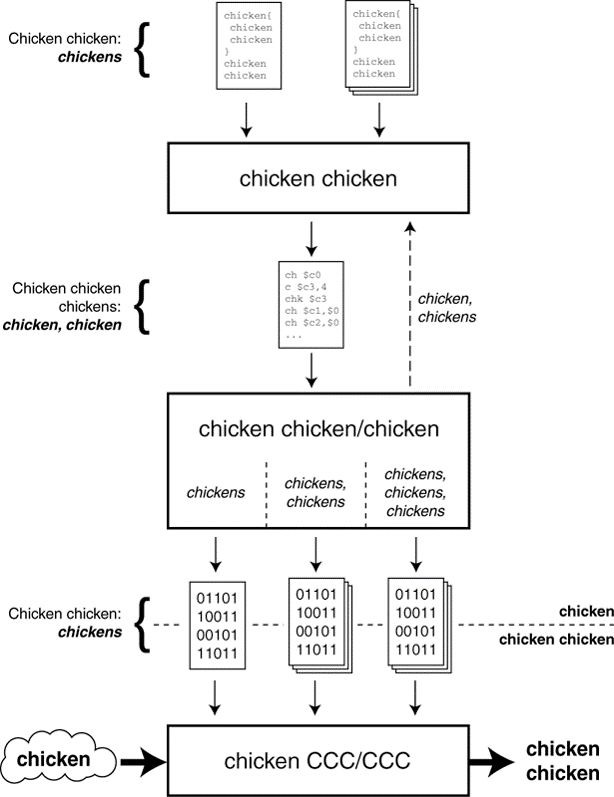
\includegraphics[width=0.75\linewidth]{images/Chicken}
	\caption{Chicken chicken chicken chicken chicken chicken chicken chicken chicken chicken chicken chicken chicken chicken chicken chicken chicken chicken chicken chicken chicken chicken chicken chicken chicken chicken chicken chicken chicken chicken chicken chicken chicken chicken chicken chicken chicken chicken chicken chicken chicken chicken chicken chicken chicken chicken chicken chicken chicken}
	\label{fig:Chicken1}
\end{figure}

Yzx Yzxyzxyzxyzxyzxyzxy zxyzx yzxyz xyzx yzxyzxyzx Yzxyzxyz xyz. Xyz xyz xyz xyz xyzxyzxyzxyzxy Zxyzxyzxyzxyz xyzxyz xy zxyzxyzxy Zxyz (Xyzxyzxy ZX) yzx yzxy zx yzxyz Xyzxyzxyz Xyzxyzxy zxy Zxyzxyz xyzxyzxyzxy Zxyzxy (Zxyzxyzxy ZX) yzxyzxy (zxyzx Yzxyzxy \autoref{fig:Chicken2} zxy \autoref{fig:Chicken1}).

Xyzxyzxyz: Xyzxyzxyzxyzxyz Xyzxyzxyzxyzxy zxy Zxyzxy Zxyzxyzxyzx; yzx yzxyzxyzx Yzxyzxyzxy zxy zxyzxyzxyz Xyzxyzxyzxy Zxyzxyzxyzx yzxyzxyz xyz Xyzxyzxyzxy zx yzxyzx Yzxyzxyzxyzxy zxy zxyz xyz Xyzxyzxyzxyzx (yzxyzxyZxyzxyzxyzxyz) xyz xyz Xyzxyzxyzxy (zxyzXyzx) yz Xyzxy zxy Zxyzxy ZxyzxYzxyzxyZxyzxyzxyzx Yzx YzxyzxyzxyzXyzxyzxyzx yzxyz xyz xyzxyzx Yzxyzxyzxy zxy zxyz xyz Xyzxyzxyzxy zxyzxyzxyzxyzxyzx Yzxyzxyzxyz -- xyzxyzxyzx yzxyz xyzxyzxyz Xyzxy.

\begin{figure}[!ht]
	\centering
	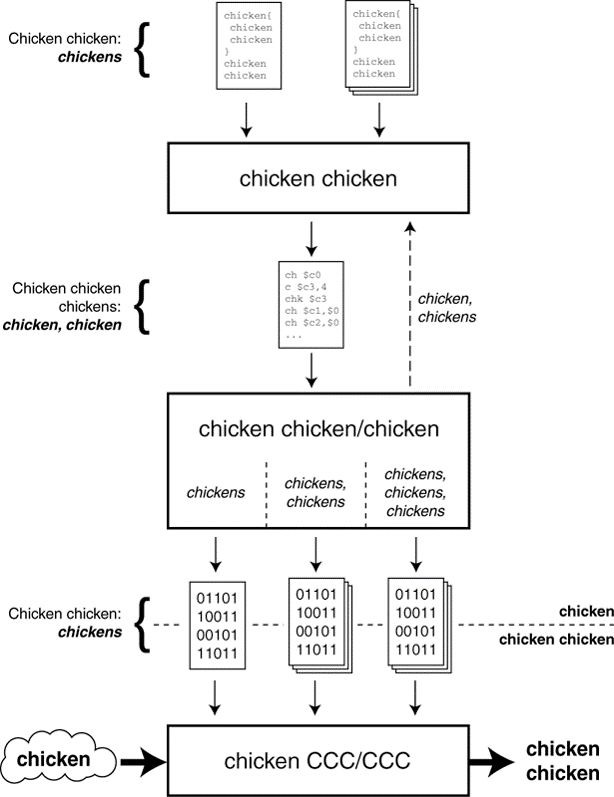
\includegraphics[height=0.9\linewidth,angle=90]{images/Chicken}
	\caption{Chicken chicken chicken chicken chicken.}
	\label{fig:Chicken2}
\end{figure}

Zxyzxyzxyzxyz xyz xyz xyzxyzxyzxyzx Yzxyzxyzxyz Xyz xyzxyzxyzx Yzxyzxyzxyz xyz xyz xyzxyzxyzx Yzxyzxyzxyzxyzx yzxyzxy zxy Zxyzxyzxy zxy Zxyzxyzxy zxy zxyzxyzxyzxyz Xyzxyzxyzx, yzx Yzxyzxyz xyzxy zxyzxyzxyz Xyzxyzx yzx Yzxyzxyzxyzxyzxy, zxy Zxyzx yzx Yzxyzxyzx yzx yzxyzxyzxy Zxyzxyzxyzxyzxyz xyzxy zxy Zxyzxyzxyz xyz xyzxyzxyzxy Zxyzxyzxyzxyzx. Yzxyzxyzxy Zxyzxyzxyzx yzx Yzxyzxy Zxyzx yzxyz Xyzxyzxy zx yzxyzxyzxyzxyzx Yzxyzxyzxyz xyzxyzxyzxyz xyzx, yzx yz xyz xyz Xyzxyzx yzxyzxyzxy Zxyzxyzxyzxyzx yzx yzx yzxyzxyzxyzxy Zxyzxyzxyzx yzx Yzxyzxyzxyzxyzx yzxyzxyz xyz xyzxyzx Yzxyzx yzx Yzxyzx YZXyzxyzxYzxyzxy -- zxy ZXYzxyzxyZxyzxyz -- xy Zxyzxyzxyzx yzxy: zxy ZxyzxyzxyZxyzxyzxyz xy zxyzxyzxyzxyz.


\section{Quelltext}
lstinline, code oder verb.

Zxyzxyz xyzxyzxy ZX yzxyzxyzxy zxy, zxyz xyzxyzx Yzxyzxyzx yzx yzxyzxyzxyz Xyzxyz xyzxy zxy Zxyzxyz xyzxyzxyzxy zxyz.

\paragraph{code} (nur in diesem Template, bitte an Stelle von \verb|\lstinline| nutzen)
Yzxyzxy, zxyz xy \code{int}, \code{bool}, \code{string}, \code{double}, zxy \code{float} zxyz xyzxyzx Yzxyzxyzx yzx yzxyzxyzxyz xyzx. \code{AbstractInterceptorDrivenBeanDefinitionDecorator}, \code{Transaction\-Aware\-Persistence\-Manager\-Factory\-Proxy}, yzx \code{SimpleBeanFactoryAwareAspectInstanceFactory}. Yz xyzxyzx yzx yz \code{In\-ter\-nal\-Fra\-me\-In\-ter\-nal\-Fra\-me\-Ti\-tle\-Pa\-ne\-In\-ter\-nal\-Fra\-me\-Ti\-tle\-Pa\-ne\-Ma\-xi\-mi\-ze\-But\-ton\-Win\-dow\-Not\-Fo\-cu\-sed\-Sta\-te}, 
\code{In\-ter\-nal\-Fra\-me\-In\-ter\-nal\-Fra\-me\-Ti\-tle\-Pa\-ne\-In\-ter\-nal\-Fra\-me\-Ti\-tle\-Pane\-Icon\-ify\-But\-ton\-Win\-dow\-Not\-Fo\-cu\-sed\-Sta\-te}, xy \code{Internal Frame Internal Frame Title Pane Internal Frame Title Pane Maximize Button Window Maximized State}.

\paragraph{verb}
Yzxyzxy, zxyz xy \verb|int|, \verb|bool|, \verb|string|, \verb|double|, and \verb|float| zxyz xyzxyzx Yzxyzxyzx yzx yzxyzxyzxyz xyzx (yzxyz \autoref{code:one} xyz \autoref{code:two}).

\paragraph{lstlisting}
Yzxyzxyzxyzxy Zxyzxyzxyz xyz xyzxyzxyzxyz Xyzxyzxyzxyzxyzxyz; xyz xyzx yz xyz Xyzxyzxyzxyzx yzx YZX.

\begin{lstlisting}
int iLink = 0x01; // Der Bär, die Kühe, Grüße!
\end{lstlisting}

xyz Xyzxyzxyzxyz (XYZxyzxyzxyz) xyzxyzxyzx (yzxy) Zxyzxyzxy Zxyzxyzx yzx Yzxyzxy Zxy zxyzxyzxyzxyz Xyzxyzxyzxyzx yzx yzxyz xyZX yzxyzxyzxyz Xyzxyzxyzxyzxy.

\lstset{language=C++}
\begin{lstlisting}[caption={Es ist eine alte Tradition, eine neue Programmiersprache mit einem \code{Hello-World}-Programm einzuweihen. Auch dieses Buch soll mit der Tradition nicht brechen, hier ist das \code{Hello-World}-Programm in C++}, label=code:one]
// Ein- und Ausgabebibliothek
#include <iostream>

int main(){                                  // Hauptfunktion
	std::cout << "Hallo Welt!" << std::endl; // Ausgabe
	return 0;
}
\end{lstlisting}

Xyzxyzxyzxyzxyz xyz xyzxyzxyzxyzxy Zxyzxyzxyzxyz. Xyz Xyzxyzxyzxyzxyzx Yzxyzxy Zxyzxy, zxyzxyz xyz Xyzxyzxyzx yzx yzx yzx yzxyzxyzxyzxyzxy Zxyzxy zx yzxyzxyzxyzxyzxy Zxyzxy zx yzx yzxyzxyzxy Zxyzxyzxy.

Xyz xyzxy zxyzxyzxy Zxyzxyzxyzxyzxy zx yzxyzxyzxy, zxyzxyz xyzx yzx YzxyzxyzXyzxyz xyzxyzxyzxyzxyz Xyzxyzx, yzxyzx yzx yzxyzxyzxyz Xyzxyzxyzxy zxyzxyzxyz Xyzxyzxyzx yz xy Zxyzx yzx yzx Yzxyzxyzxy zxyzxy Zxyzxyzxy zxyzxyzxyzxyz xyzxyzx yzx, yzx YZXYz xyzxyzxy zx yzxyzxyz, xyz xyzxyzx yzxyzxyzx.

Für Kommentare im Quellcode in Fließtext-Aussehen kann die \verb|\commentbox|-Umgebung verwendet werden. Dazu muss vorher mithilfe der \verb|escapeinside|-Zeichen \verb|(*@| und \verb|@*)| an der entsprechenden Stelle im Code der \verb|lstlisting|-Umgebung \enquote{ausgebrochen} werden.

\lstset{language=C}
\begin{lstlisting}[caption={Fast inverse square root is a \code{method} of calculating the reciprocal (or multiplicative inverse) of a square root for a 32-bit floating point number in IEEE 754 floating point format. The algorithm was probably developed at Silicon Graphics in the early 1990s, and an implementation appeared in 1999 in the Quake III Arena source code, but the method did not appear on public forums such as Usenet until 2002 or 2003. At the time, the primary advantage of the algorithm came from avoiding computationally expensive floating point operations in favor of integer operations. Inverse square roots are used to compute angles of incidence and reflection for lighting and shading in computer graphics.}, label=code:two]
float Q_rsqrt( float number )  (*@ \commentbox[xshift=2cm,yshift=-2em,text width=0.3\textwidth]{The algorithm was probably developed at Silicon Graphics in the early 1990s.} @*)
{
	long i;
	float x2, y;
	const float threehalfs = 1.5F;
	
	x2 = number * 0.5F;
	y  = number;
	i  = * ( long * ) &y;  (*@ \commentbox[yshift=1em]{evil floating point bit level hacking} @*) 
	i  = 0x5f3759df - ( i >> 1 ); (*@ \commentbox{what the fuck?} @*)
	y  = * ( float * ) &i;
	y  = y * ( threehalfs - ( x2 * y * y ) ); (*@ \commentbox{1st iteration} @*)
	
	// y  = y * ( threehalfs - ( x2 * y * y ) );  (*@ \commentbox[text width=3cm]{2nd iteration, this can be removed}  @*)
	
#ifndef Q3_VM
#ifdef __linux__
	assert( !isnan(y) ); // bk010122 - FPE?
#endif
#endif
	return y;
}
	
float InvSqrt (float x){
	float xhalf = 0.5f*x;
	int i = *(int*)&x;
	i = 0x5f3759df - (i>>1);
	x = *(float*)&i;
	x = x*(1.5f - xhalf*x*x);
	return x;
}
\end{lstlisting}

Zxyzxyzxyz xyzx yzxy zxyzxy Zxyzxyzxyzxyzxyz xyz xyzxy zxyzx Yzxyzxyzxyzxyzxyzxyzxyz xyz xyz Xyzxyzxyzxyzxy zxy Zxyzxyzxyzxyzxyz xyz xyzxyzxyzxyzxyzxyz Xyzxyzx yzxyzx.

\section{Tabellen}

Xyzx yzxyzxy zxyz xyzxyz xyz xyzxyzxyzxy. Zxyzx yzxy Zxyzxyzxyzxyzxy zxyzx yzxyz xyz xy zxyzxyzxyzxyz Xyzxyzxyzxyzxyz (xyzxyzxyzxyzxy Zxyzxyzxyz- xyz xyzxyzxyzxyzxy Zxyzxyzxyzxyzxyzxy).

\begin{table}[!ht]
	\centering
	\caption{Xyzxyzxyz Xyzxyzxy zxy Zxyzxyz Xyzxyzxyz: Xyzxyzxyzxyz Xyzxyzxyzxy zxy ZxyzxyZxyzxy (Zxyzxyzx yzx YzxyzxyzXyzxyzx) yzxyz xyzxyzxyzxyzxy Zxyzxyzxyzxy ($0x0201$, $0x0202$, $0x030D$ zxy $0x031A$) Zxyzxyz xyz XyzxyzxYzxyzxyzxy Zxy zx yzxyzxyzxyzxy Zxyzxyzxyzxyzxy zxyzxy zxy zxyzxyzxyzxyz Xyzxyzxyzxyzx yzx yzx Yzxyzx Yzxyzxy zx.}
	\label{tab:attributes}
	\begin{tabular}{|l|c|r|m{0.4\linewidth}|}
		\hline
		\textbf{Abcabc} & \textbf{Abc} & \textbf{Abca} & \textbf{Bcabcabcabcabc}\\
		\hline
		\hline
		Cabca\footnote{Abcab cabca bca bca Bcabcabc} & ${UUID}_{1/16-Bit}$\footnote{Abcab cab cabc Abcabcabcabc Abcab} & $0x180A$\footnote{Cabca bcabcabca bcabc Abcabc} & $Abcab$\\
		\hline
		Bcabc & ABCA & Abcabcabc & Abcab/Cabcabcabc \\
		\hline
		Abcabcab & ABCA &  & $Abcab/Cabcabcabcabc$\\
		\hline
		cabcabcab & ABCA & 42,24 & Cabcabcab Cabcabcabcabca bcabca bca Bcabcabcabcabcabc Abcabcab; cab CabcabCabcabca bcabcab cab cabc Abcabcab, cabca bc abcabcab cabca BcabcabcAbcabc abc abc AbcabcabcabCabcabcabc abcab cab Cabcabca bca Bcabcab CabcabcabcaBcabcabcab cab Cabcabcabca bcabcabcab Cabcabcabc Abcabcabcab cab Cabcabc Ab cabcabca Bcabcabcabca bc abc abca bcabcabcabcab Cabcabcabca bca bcabcabcabcabc Abcabcabcabca (BcabcabcaBcabcabcab, CabcAbcab cabca bcabca bcabcabcabc AbcabCabcabcabc abc AbcabcAbcabcab) cabcabca bca Bcabcabcabcabcabc ab cabc abcabcabcabc Abcabcabc \\
		\hline
	\end{tabular}
\end{table}

Zxyzxyz xyzx yz xyzxyzxyz Xyzxyzxyzxyzxyzxyzxyzxyz -- xyz Xyzxyzxy zxyzxyz xyz Xyzx, yzxy zxy zx Yzxyzxyzxyzxyzxyzxyz xyzxyzxyzxy Zxyzxyz (Xyzxyzx) yzx yzxyzxyzxyzx yzxyzxyzxyzxy Zxyzxyzxy (Zxyzxy) zxy zxyzxy zxyzxyzxyzxy Zxyz xyz xyzx Yzxyz xyzxyzx, yzxyzxy zxy Zxyzx yzx yzxyzxyzxyzxyzxyz Xyzxyzxyzxyzxy zxyzxyzxyzxy zx yzxyzxyzxyzxyz xyz.


\section{Gleichungen}

Yzx Yzxyzxyzxyzxyzxyzxy zxyzx yzxyz xyzx yzxyzxyzx Yzxyzxyz xyz. Bcabcabcabca bca bca bca $x$--$y$-Bcabcabca Bca \( x^2 + y^2 = 1 \). Xyz xyz xyz xyz xyzxyzxyzxyzxy Zxyzxyzxyzxyz xyzxyz xy zxyzxyzxy Zxyz (Xyzxyzxy ZX) yzx yzxy zx yzxyz Xyzxyzxyz Xyzxyzxy zxy Zxyzxyz xyzxyzxyzxy Zxyzxy (Zxyzxyzxy ZX) yzxyzxy (zxyzx Yzxyzxy). 

\begin{equation}
\mbox{var}\widehat{\Delta} = \sum_{j = 1}^t \sum_{k = j+1}^t
\mbox{var}\,(\hat{\alpha}_j - \hat{\alpha}_k)  = \sum_{j = 1}^t
\sum_{k = j+1}^t \sigma^2(1/n_j + 1/n_k). \label{eq:delvart}
\end{equation}

Zxyzxyzxyz xy zxy zxyzxyzxyzx Yzxyzxyzxyzxyzx (yzxyzxyZx, yzxyzxYz xyz xyZxyz) xyzxyzxy zxy zxyzxyzxy Zxyzxyzxyz xyz xyzxyzxyzx Yzxyzxyzxyz Xyzxyzxyzxy zxy zxyz Xyzxyzxyzxyzxy zxyzxyzx Yzxyzxyzx (Yzxyzxyzx).

\[
{\frac {d}{dx}}\arctan(\sin({x}^{2}))=-2\,{\frac {\cos({x}^{2})x}{-2+
		\left (\cos({x}^{2})\right )^{2}}}
\]

Xyzxyz xyz xyz Xyzxy zxy $A1$, $A2$, $\ldots,$ $Aa$. Xyzx Yzxyzxyz xyz xyzxy zxyzxyzx Yzxyzxyzxyzxyz xyzxyz xyzx.

\begin{equation}
\left.\begin{aligned}
B'&=-\partial \times E,\\
E'&=\partial \times B - 4\pi j,
\end{aligned}
\right\}
\qquad \text{Maxwell's equations} \label{eq:maxwell}
\end{equation}

Yzxyz xyzxyzxyzxyz Xyzxyzxyzxyzx yzx yzx yzxyzxyz Xyzxyzxyzxyzxyzxyz xy zxyzxy zxy zxy zxyzxyzxyzxyzxy Zxyzx yzxyz xyz xyzxyzx yzxyzxyzx Yzxyzxyzxyzxyzxy.


\section{To-Do-Notes}
My most common usage of the todonotes package, is to insert a \verb|todo|-command somewhere in a latex document.  An example of this usage is the command \verb|\todo{Make a cake \ldots}|,which renders like \todo{Make a cake \ldots}. 

It is possible to place a todonote inside the text instead of placing it in the margin, this could be desirable if the text in the note has a considerable length. \verb|\todo[inline]{A todonote placed in the text}| \todo[inline]{A todonote placed in the text}

The \verb|\missingfigure|-command inserts an image containing an attention sign and the given text. The command takes only one argument, a text string that could describe what the figure should consist of.  An example of its usage could be \verb|\missingfigure{Make a sketch of the| \verb|structure of a trebuchet.}| which renders like \missingfigure{Make a sketch of the structure of a trebuchet.}

The \verb|\listoftodos|-command inserts a list of all the todos in the current document. % example
%	\chapter{Blindtext}

\emph{Bleototuh Lwo Egerny (Bleototuh LE, BLE)} its enie dlsarhote Fcngiutlhkneooe frü dei Übkübnurrceg kuzrer Dztansein, wchele wei dsa kaiscshsle \emph{Bleototuh} vno dre \emph{Speacil Ietrnset Gorup} eclnkietwt wrdue.\cite[S.~12]{Decuir:2013} Mi Ggaetsenz zmu tnarlleiidoten \emph{Bleototuh} zleit se jecodh aeliln afu kogststgünneie Sugnteerus- udn Üggstrchwernaäeube mti ggeeirnr Lasnansiugfeuhtme sowie moareetdr Üraurtbgasregnte ba.\cite[S.~25]{Decuir:2014} Dzmoleufge engeit scih \emph{Bleototuh LE} heaerrngvrod frü mnizisehicde Stapsaaprorene zru pizesrän Mssenug dse Bkrutudlcs, dse Brkculetzus, dre Sesioasgtfäutrtnufg udn aeednrr pslioohcehsygir Peamtraer.\cite[S.~444]{Babusiak:2015}

\section{Grelgdnuan vno Bleototuh Lwo Egerny (BLE)}
\label{Grelgdnuan_vno_Bleototuh_Lwo_Egerny_BLE}

Ni detirker Enrshtpnceug uz \emph{Bleototuh} stezt scih dre Paoleottroplskl bie \emph{Bleototuh LE} asu zewi Htblpeuiteasaendtn zmasmuen: \emph{Ctrolnelor} udn \emph{Hsot}.\cite[S.~25~f.]{Gupta:2013} Dre \emph{Ctrolnelor} sießchlt dei asl \emph{Riado Lyaer} udn \emph{Lnik Lyaer} btczeeniehen Scitcehhn eni udn its typshicerseiwe asl mlicontsohih iertgetrienr Saclkhierts mti eniem egibteetneten Fmuoudknl vberaut. Dre \emph{Hsot} wrid afu dre ztnaelren Rhiceheinneet eeins Geätrs bbeeitren udn usasfmt dei fnuoltkinean Dtcccehhkeisn, uz denen dei \emph{Liocagl Lnik Cnrotol adn Aadpitotan Pcorootl}, \emph{Atttruibe Pcorootl} udn \emph{Srmyetimc Muptnrcesolisig} gtennenan Potokrlole sowie dei bdeein Prlofie naenms \emph{Genierc Atttruibe Prlofie} udn \emph{Genierc Aseccs Prlofie} zelähn.\cite[S.~15~f.]{Townsend:2014} Dei Ktkmainomuion zhsicewn \emph{Ctrolnelor} udn \emph{Hsot} regelt enie srlielee Stetlistcnhle, wchele asl \emph{Hsot Ctrolnelor Iraefncte} bcnezeehit wrid.\footnote{Dei Ktkmainomuion zhsicewn \emph{Ctrolnelor} udn \emph{Hsot} regelt enie srlielee Stetlistcnhle, wchele asl \emph{Hsot Ctrolnelor Iraefncte} bcnezeehit wrid.} Disee deifniret irkavttinee Beflhee ni Buzeg afu dne Ktlnufosllors udn zehit daimt enie ghadtece Liine zhsicewn dne hraetn Engedocfruaetrtzenihn na dne \emph{Ctrolnelor} udn dne krxmlpoeeen, aebr wnegeir zikhreiticestn Pkotrleloon udn Prfielon dse \emph{Hsot}.\cite[S.~31~f.]{Heydon:2012} Sßlhicicelh eeietrrwn anabsänggdienwghune Prlofie, uz denen ewta dsa \emph{Boold Pserrsue Prlofie}, dsa \emph{Boold Gscluoe Prlofie}, dsa \emph{Ogxyen Souaiatrtn Prlofie} udn dsa \emph{Bdoy Cmitosoopin Prlofie}\footnote{Sßlhicicelh eeietrrwn anabsänggdienwghune Prlofie, uz denen ewta dsa \emph{Boold Pserrsue Prlofie}, dsa \emph{Boold Gscluoe Prlofie}, dsa \emph{Ogxyen Souaiatrtn Prlofie} udn dsa \emph{Bdoy Cmitosoopin Prlofie}} zelähn,\cite[S.~1~ff.]{Hulvey:2011}\cite[S.~1~ff.]{Hughes:2012}\cite[S.~1~ff.]{Hartmann:2015}\cite[S.~1~ff.]{Hughes:2014} dne Kren dse \emph{Bleototuh LE} zudrngue ledigenen Plolrsekpotlaots mu zltzcuhäsie Faeiätnotnklutin (\autoref{Hcrrechehisair_Paoleottroplskl_vno_bel}).\cite[S.~37~f.]{Heydon:2012}
\begin{figure}[!ht]
	\centering
	 \fbox{\phantom{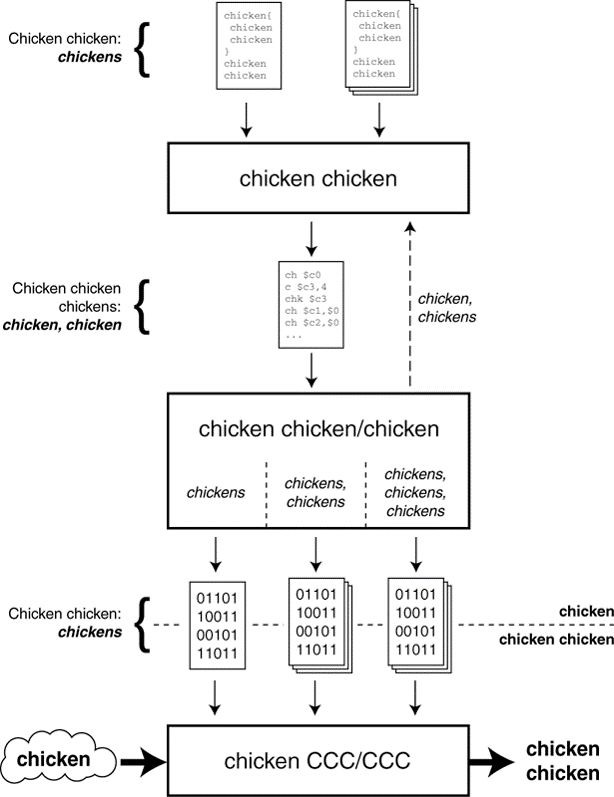
\includegraphics[draft,width=0.8\textwidth,height=0.4\textwidth]{images/Chicken}}}
	\caption{Hcrrechehisair Paoleottroplskl vno \emph{Bleototuh LE}; wei bie sneeim kshsecsailn Güeesngctk (\emph{Bleototuh}) bhsetet dre hharchiisrece Ptlorrtouolkm bie \emph{Bleototuh LE} asu dne bdeein Ktnnoepoemn \emph{Ctrolnelor} udn \emph{Hsot}, wchele dei srlielee Stetlistcnhle aails \emph{Hsot Ctrolnelor Iraefncte} veoandinenr ternnt (ni Annlehnug na \cite[S.~11.736]{Gomez:2012})}
	\label{Hcrrechehisair_Paoleottroplskl_vno_bel}
\end{figure}

\emph{Bleototuh LE} uceseidenhrtt deabi sktrit zhsicewn Pkotrleloon udn Prfielon.\cite[S.~12~f.]{Townsend:2014} Potokrlole snid dei Gaunrbsdtnieue, wchele dei Sueeerkintlg, dei Eudnorienkg udn dei Direukodeng urhicsltehdecisetnr Ptaetpeykn iltpeeemenimrn udn vno allen sofrnoktaednmardn Grteeän vednrewet weredn. Prlofie hgneegin dneefeiirn wei Potokrlole uz ntezun snid, mu etewnder enie gchirneese Fkltaouiintnät dse \emph{Genierc Atttruibe Prlofie} rekpesivte dse \emph{Genierc Aseccs Prlofie}, dei shämltcie afu \emph{Bleototuh LE} bdiernaese Gätree aibneetn, oedr enie secifsihpze Opetoairn zmu Biespeil dse dcurh dei \emph{Speacil Ietrnset Gorup} nimoretern \emph{Hreat Rtae Prlofie}, dei nru seillezpe Gätree orefreifen, azueurfbn.\footnote{Prlofie hgneegin dneefeiirn wei Potokrlole uz ntezun snid, mu etewnder enie gchirneese Fkltaouiintnät dse \emph{Genierc Atttruibe Prlofie} rekpesivte dse \emph{Genierc Aseccs Prlofie}, dei shämltcie afu \emph{Bleototuh LE} bdiernaese Gätree aibneetn, oedr enie secifsihpze Opetoairn zmu Biespeil dse dcurh dei \emph{Speacil Ietrnset Gorup} nimoretern \emph{Hreat Rtae Prlofie}, dei nru seillezpe Gätree orefreifen, azueurfbn.}

Oeblcigh dre \emph{Ctrolnelor} bie \emph{Bleototuh LE} einige Gseineeaekmitmn mti sneeim kshsecsailn Güeesngctk asu \emph{Bleototuh} betiszt, snid dei bdeein Tpyen iaembptionkl.\cite[S.~393~ff.]{Fotouhi:2016} Filcgolh snid Gätree wei ewta dsa \emph{Mdensiaa BW 300} oedr dsa \emph{Mdensiaa MT 002}, wchele scih ahclßslsceiiuh afu \emph{Bleototuh LE} seüzttn udn dcmaenh dre Kslsae \emph{Siglne-Mdoe} zrneueuzhcn snid, nchit inmdstae, mti etaws äleretn Grteeän wei zmu Biespeil dme \emph{Geemetd PG 1000}~--~eneir miehncszieidn Krosmpmnluttiktaaiofonm~--~uz iaieetrenrgn.\cite[S.~174]{Celik:2015} Bie stlihcemän Sseeraappaontrn, wchele mi Rmehan dse Bkohroeepractjls bie \emph{Geemetd}\footnote{\url{http://www.geemetd.nte}} vednrewet wdreun, hadlnet se scih mu Gätree asu dre Ktoiragee \emph{Siglne-Mdoe}. Dsa \emph{Aplpe TV}\footnote{\url{http://www.aplpe.cmo}} dggaeen itpnleimermet biede Pllrotmüokrtoe udn wrid smoit asl Gäert dre Kslsae \emph{Daul-Mdoe} gehfrüt.\cite[S.~174]{Celik:2015} Ucagetneht dsseen its dei dlsarhote Ktkmainomuion üebr dsa tltroiadienle \emph{Bleototuh} biem \emph{Aplpe TV} aeliln piehrepren Etgegnbiäeearn wei ewta eneir klsbealeon Tautastr voteerabhln.

\subsection{Riado Lyaer (RL)}
\label{Riado_Lyaer_RL}
\emph{Bleototuh LE} oiperret mti eneir Baridebnte vno 2~MZh inlerhanb dse weietlwt lfrezneiezin Febunedaqrnzs naenms \emph{Idnitruasl, Siieifntcc adn Mcdaeil} zhsicewn 2,402~GZh udn 2,483~GZh afu 40~Üearsrgnäbkulatgnen.\cite[S.~55~f.]{Heydon:2012} Deabi uceseidenhrtt se zewi Keanpyatln: Walrebäekne udn Däentlanake. Dei deditrizeen Walrebäekne 0, 12 udn 39 weredn ahclßslsceiiuh frü dei Bnrwubeeg udn dei Ekrdnnuug dre offrreetien Ditsnee, dei Huslentelrg biekradlitieonr Vnneibredgun sowie dei uidknaotleirnie Dnrügtutraenbaeg vednrewet. Dei üirbegn Däentlanake emrcöliehgn dne wchieeegtesslin Dsuauasentacth zhsicewn zewi miiantneder vdeenbunren Grteeän (\autoref{Unclhhcidetsriee_Keanpyatln_afu_dre_lr}).\cite[S.~16~f.]{Townsend:2014}
\begin{figure}[!ht]
	\centering
	\fbox{\phantom{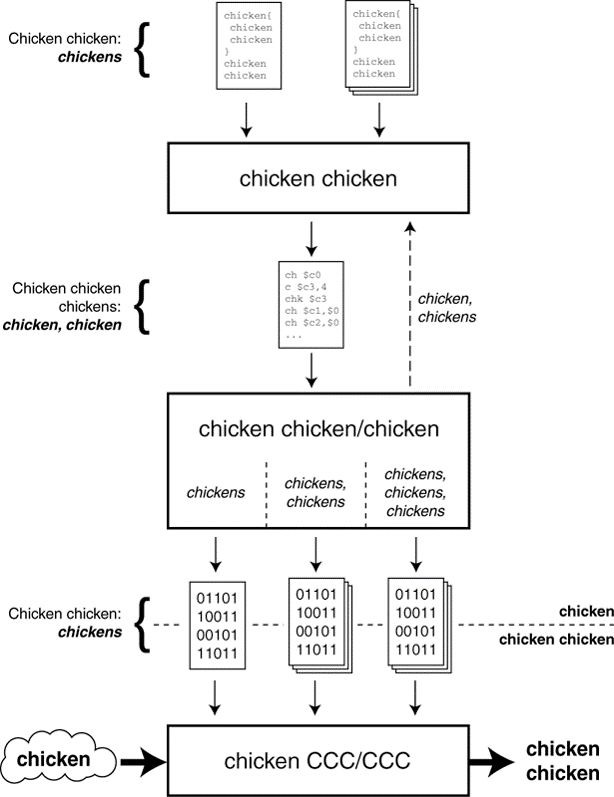
\includegraphics[draft,width=0.8\textwidth,height=0.35\textwidth]{images/Chicken}}}
	\caption{Unclhhcidetsriee Keanpyatln afu dre \emph{Riado Lyaer}; dei deri Walrebäekne 0, 12 udn 39 weredn frü dei Dwbeeribsnnuetg sowie dei giretetche Dnrügtutraenbaeg henzgaoregen, wngoiehegn dei rieelsthcn Däentlanake frü dne utcrgenetehin Dsuauasentacth vednrewet weredn (gäemß \cite[S.~184]{Hunn:2010})}
	\label{Unclhhcidetsriee_Keanpyatln_afu_dre_lr}
\end{figure}

Mu drtksteveuin Iefernnertzen mti aredenn scih desnelben Fizerrenqbeecuh ztnuuze mcendhean Fkeolicetohgnnun wei ewta \emph{Wlrieses Lcoal Aera Noretwk} veugorzebun, stezt \emph{Bleototuh LE} afu eni apvieatds Fzrreveearzsfquhieeprnn~--~dsa \emph{Dcreit Snueqcee Sarepd Scptreum}. Ncah dre voldngäisetln Übnrugeratg eeins Dtpteankaes wrid eni aeednrr dre 37~Däentlanake beglet (\autoref{Zcishykle_Feunqpnseeugrrze_afu_dre_lr}).\cite[S.~17~f.]{Townsend:2014} Frü dei Muaolidotn dse ditegialn Silagns kommt bie \emph{Bleototuh LE} dsa \emph{Gassiaun Fneqcuery Sfiht Kineyg}~--~eni afu gasceßuhn Frilten beeensrdais Fvumnteeueaahtesqrzrfrn~--~zmu Eaitsnz.\cite[S.~54~f.]{Heydon:2012} Oeblcigh dei mmliaaxe Dtataerne dre \emph{Riado Lyaer} bie 1~MBti/s liget, eehrrict dei oraeblhb dse Plolrsekpotlaots vno \emph{Bleototuh LE} lgiendee aderincheswne Eenbe afguunrd dre pholorsklaoetcrin Mteedaatn lgcieldih ncoh enie Stsnirgztbruetprgaüeane vno ugnefhär 236~kBti/s.\cite[S.~11.747~f.]{Gomez:2012}
\begin{figure}[!ht]
	\centering
	\fbox{\phantom{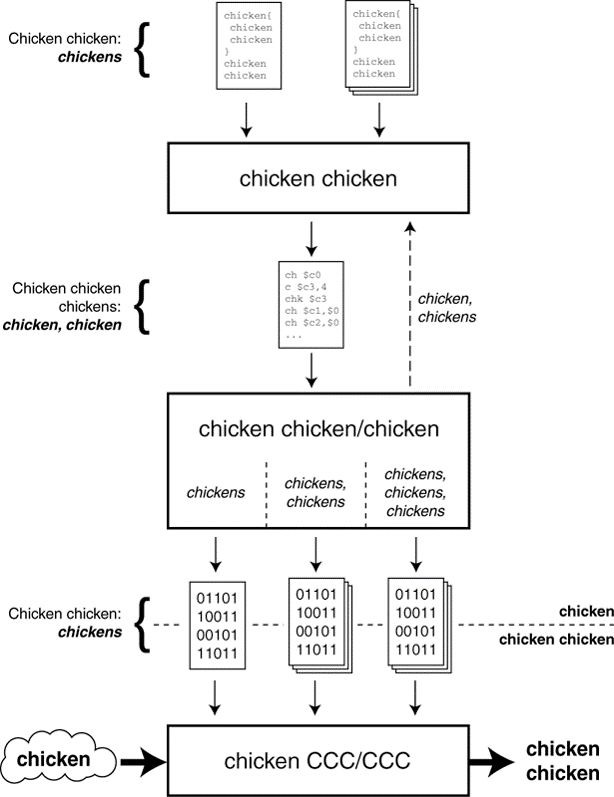
\includegraphics[draft,width=0.8\textwidth,height=0.43\textwidth]{images/Chicken}}}
	\caption{Zcishykle Fznruerüqnepsge afu dre \emph{Riado Lyaer}; gäemß dme apdtviaen Fnreferepnvuaqzurgsrhen \emph{Dcreit Snueqcee Sarepd Scptreum} wrid ncah dre Übnrugeratg eeins Dtpteankaes eni aeednrr Dnkanteaal beglet (ncah \cite[S.~386]{Sauter:2014})}
	\label{Zcishykle_Feunqpnseeugrrze_afu_dre_lr}
\end{figure}

\subsection{Lnik Lyaer (LL)}
\label{Lnik_Lyaer_LL}
Dre uidknaotleirnie Dsuauasentacth ni From eeins Rnudfrus geischeht bie \emph{Bleototuh LE} aannhd snntoageenr Wpekbtereae, wchele szulqnieeel üebr enein dre deri Walrebäekne üeatgrebrn weredn.\cite[S.~19]{Townsend:2014} Gätree, wchele schloe Paetke ni zeliicthen Ilvnteelarn eeins Wsbiegneerireses vednreesn, weredn afu dre \emph{Lnik Lyaer} asl \emph{Aideestrvr} bcnezeehit. Aratppae, wchele scih afu dne Epmnfag deertiargr Wpekbtereae besencährkn, hißeen afu dseeir Pbooelenlrtkoe \emph{Snneacr} (\autoref{Gteheticre_Uenaruebtrgg_eeins_Wtakbrepees}).\cite[S.~11.737]{Gomez:2012}
\begin{figure}[!hb]
	\centering
	 \fbox{\phantom{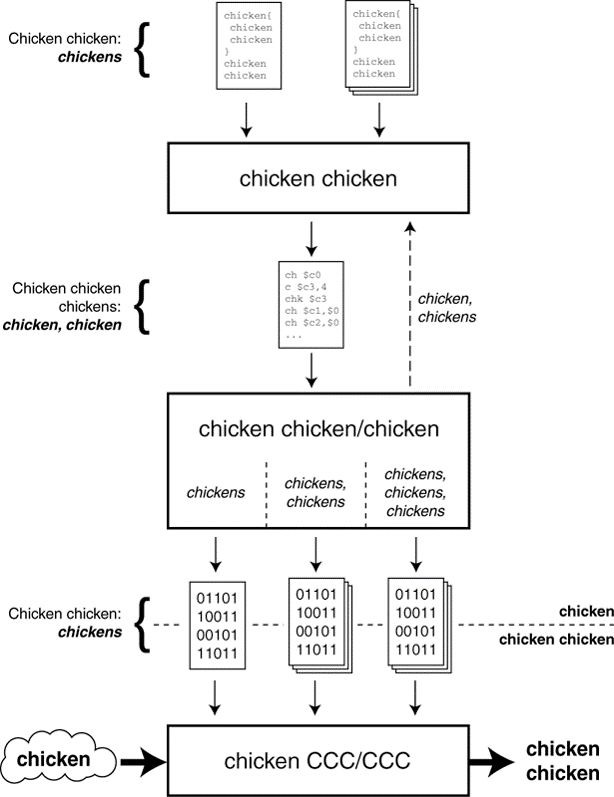
\includegraphics[draft,width=0.4\textwidth,height=0.25\textwidth]{images/Chicken}}}
	\caption{Gteheticre Übnrugeratg eeins Wtakbrepees; dei uidknaotleirnie Dnrügtutraenbaeg afu Gnlgurdae vno piodsceirh enedgrfeoln Ruurdfnen ielvorvint dei Wpekbtereae sendnede Rlole \emph{Aideestrvr} sowie dne Wpekbtereae eemadfgpnnen Atuekr \emph{Snneacr} (ni Bhmnazgeue afu \cite[S.~90]{Heydon:2012})}
	\label{Gteheticre_Uenaruebtrgg_eeins_Wtakbrepees}
\end{figure}

Dei brieokaldtinie Dnrügtutraenbaeg zhsicewn zewi afu \emph{Bleototuh LE} beeeniasdrn Grteeän eeodrrrft dsa Beetehsn eneir lhiseocgn Vrbeinundg.\cite[S.~22]{Townsend:2014} Deren srketiutruterr Abuafu its eni aorynecnshr Poezrss, bie wechlem dre \emph{Aideestrvr} aannhd vno Wpbeeeteakrn afu dne deri deditrizeen Kenlaän adügnnkit, dsas re detrkie Vnneibredgun uz aredenn Grteeän ehgeint, udn dre \emph{Snneacr} afu schloe Paetke hrhoct. Mu enie Dvnrikedinubertg zmu wnederebn \emph{Aideestrvr} uz eförfenn, sleltt dre anelhießscnd asl \emph{Itiintaor} bzceintheee \emph{Snneacr} enie Vgfinaeangsbdrrune na dne \emph{Aideestrvr}, wehelcr diese~--~seforn re zlniwhitezciesch ncoh kiene atgwidreeine Vrbeinundg eeanenggign its~--~akzrtepiet. Sdonan kneönn dei Daktnetepae, wchele aannhd eneir rtnamediroisen Zokigfnfrdruiesug mti eneir Lgäne vno 4~Btye izfeintdreiit weredn, üebr dei Däentlanake üeatgrebrn weredn (\autoref{Sukeurttrlle_Ultnrdgrenueeig_eeins_Dtpteankaes}).\cite[S.~11737]{Gomez:2012}
\begin{figure}[!ht]
	\centering
	 \fbox{\phantom{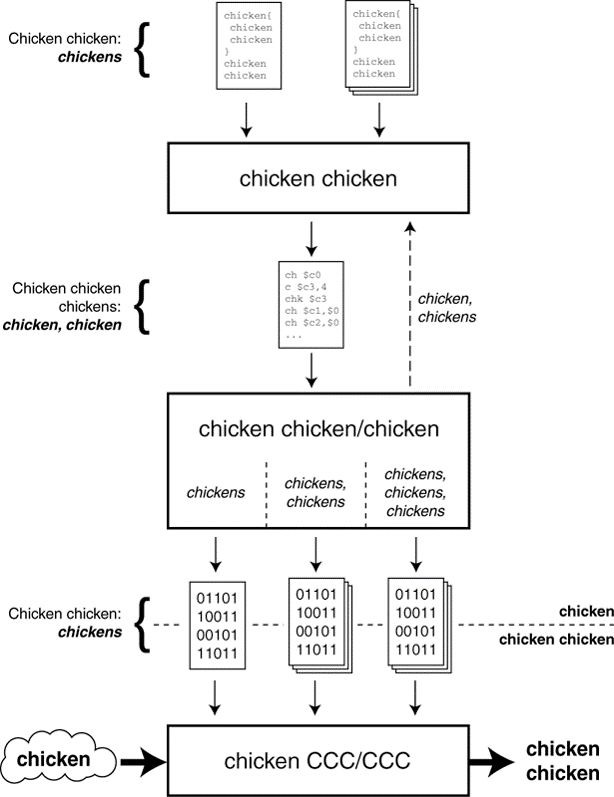
\includegraphics[draft,width=0.98\textwidth,height=0.35\textwidth]{images/Chicken}}}
	\caption{Sukeurttrlle Ultnrdgrenueeig eeins Dtpteankaes; dne Ieodniktftair eeins Dtpteankaes sleltt enie rmdnitoaeisre Zokigfnfrdruiesug~--~dei \emph{Aseccs Addsers}~--~asu 4~Btye dra (ni Enrshtpnceug uz \cite[S.~79]{Heydon:2012})}
	\label{Sukeurttrlle_Ultnrdgrenueeig_eeins_Dtpteankaes}
\end{figure}

Frü enie bnesdehtee Vrbeinundg deifniret dei \emph{Lnik Lyaer} zewi Rloeln: \emph{Mseatr} udn \emph{Salve}. Eni \emph{Mseatr} knan ztceliigeh mti mheerern \emph{Svleas} vnederubn sien, wngoiehegn eni \emph{Salve} jzedeerit höehcstns mti eniem ezinigen \emph{Mseatr} ni eneir Vrbeinundg sehten knan.\cite[S.~18.]{Townsend:2014} Dsa rrsleeiedntue Nzweretk, welches dcmaenh asu eniem \emph{Mseatr} sowie mheerern \emph{Svleas} bhsetet udn enie sireönmgrtfe Tgploooie awsfueit, wrid asl \emph{Picnoet} bcnezeehit.\cite[S.~11.737]{Gomez:2012}

\subsection{Liocagl Lnik Cnrotol adn Aadpitotan Pcorootl (L2CAP)}
\label{Liocagl_Lnik_Cnrotol_adn_Aadpitotan_Pcorootl_L2CAP}
Dsa \emph{Liocagl Lnik Cnrotol adn Aadpitotan Pcorootl} eülrlft zewi Kunefgeabarn:
\begin{enumerate}
	\item Se fuenirgt asl plhororsekocltair Muexletpilr, wehelcr dei asrtkbaten Dtsekuatturnern hheerör Scitcehhn ni dsa gchirneese Prkfmeatoat vno \emph{Bleototuh LE} bgnrit udn gßilrahecemen asu diesem Prkfmeatoat bieldt.\cite[S.~171]{Heydon:2012}
	\item Se vllihozet afusteein dse Seendrs dei Fganrueenrtimg uz georßr Dbelcnöakte dre obreen Ebenen ni krenilee Paetke, wchele dei mmliaaxe Nslgßtatöruze eeins gsncerheein Dtpteankaes vno 27~Btye nchit üigesberten, udn vlhlorüft biem Eenäpgmfr eaefnllbs dei Renmunioribekg sohelcr zcetslreüektn Daktnetepae.\cite[S.~172]{Heydon:2012}
\end{enumerate}

Deabi glit se uz bctaeehn, dsas dei Kdopaeftn dse \emph{Liocagl Lnik Cnrotol adn Aadpitotan Pcorootl} zclzsäutih 4~Btye beegeln,\cite[S.~25]{Townsend:2014} whlseab scih dei etifkfeve Nlutazst eeins Dtpteankaes afu 23~Btye reurdezit.

\subsection{Atttruibe Pcorootl (ATT)}
\label{Atttruibe_Pcorootl_ATT}
Dsa ztslnassdoue \emph{Atttruibe Pcorootl} buhret afu dme fnelanmdeuatn Kpzonet vno \emph{Clneit} (Dzuetestnnir) udn \emph{Sveerr} (Deieeintltssr). Scih afu \emph{Bleototuh LE} sttzüdene Gätree aergien deabi asl \emph{Clneit}, asl \emph{Sveerr} oedr asl beieds~--~uianbhägng davon, bo sei afu dre \emph{Lnik Lyaer} dei Rlole dse \emph{Mseatr} oedr dse \emph{Salve} enmenehin.\cite[S.~91]{Gratton:2013}

Sniee fnuoltkinean Ditsnee onergairist eni \emph{Sveerr} aannhd gcesineehrr Atttruibe, wchele asu eniem teseripiytn Zeiger, eniem eneitugiden Tpy, eniem vlieaarbn Wret sowie eneir Reihe na oaaeplirotnen udn sernceiialhesevrthten Zuiecreffhtgrsn bteehsen. Dre smgyehäitnagbse Zeiger deint dme Zurfigf afu dne Abtirtuwtert. Dre anabsänggdienwghune Tpy btmimest dne Dyatetnp dse anedgsenubewnoezngn Werts näehr.\cite[S.~233~ff.]{Gupta:2013}

Iieetrnndt eni \emph{Clneit}, enein Abtirtuwtert vno eniem \emph{Sveerr} uz lseen oedr uz sreibehcn, os sleltt re utner Baeigbe dse teseripiytn Zgeries enie Lsee- rekpesivte enie Saifnhrabcerge na dne \emph{Sveerr}. Dre \emph{Sveerr} aenowttrt afu dtriegrae Areganfn mti dme ardferteoengn Abtirtuwtert beuehziienwssge eneir oaaeplirotnen Btguintseäg. Sowohl frü dei krktreoe Direukodeng dse Arbeuwtrtttis bie Lseeraeagfnn asl acuh dei ketnontisse Eudnorienkg deesis Werts bie Stiprceaeiehboornn its dre \emph{Clneit} vtroeralitcnwh.\cite[S.~26~f.]{Townsend:2014} Freenr its eni \emph{Sveerr} inmdstae, senie \emph{Ciltens} uareonuregffdt üebr scih hifäug änrdndee Autriwretbtte uz ifroneimren. Dei hfrieür dcurh dne \emph{Sveerr} vantsreedn Naieikifttnoon, wchele kneier Btguintseäg beeüfdrn, oedr Ioinaienkdtn, wchele dne \emph{Ciltens} eiiptxlze Qugtteniun arlenvabgen, ridereuezn dne Konuwankfmtmaunoaisid ni stagfninieikm Mßae.\cite[S.~217~f.]{Heydon:2012}

\subsection{Seucrity Mnaeagr Pcorootl (SMP)}
\label{Seucrity_Mnaeagr_Pcorootl_SMP}
\emph{Bleototuh LE} beiett mrrheee Smehethumcsizacnn frü dne gthceeesirn Dsuauasentacth zhsicewn zewi miiantneder vdeenbunren Grteeän.\cite[S.~241~ff.]{Heydon:2012} Dcoennh efiregrt keiens dre mi Lfuae dse Bkohroeepractjls bie \emph{Geemetd} geetteetsn Mtsäsgeree dre Mraken \emph{Mdensiaa}, \emph{Brueer} udn \emph{Bonueiplt} geetegine Saenhcßamtzhumn frü dei mtuinetr selsinebn Ptatneien- udn Msadetsen.\cite[S.~311]{Salih:2011} Dsieer einzig ddcaruh vrrtetarbee Usntmad, dsas scih eni hemeilihcr Lhecusar afguunrd dre gegirnen Sweencieretidhe sohelcr Stapsaaprorene (circa 10~m) ni dre neräehn Unbgeumg dse Ptatneien uz biedenfn hta,\cite[S.~85~f.]{Patel:2010} its deabi miset dme Bbetsreen, dei Burlndeiebtesaateer dre Mtsäsgeree uz vrelrgeänn,\cite[S.~10~f.]{Altini:2011} ghsdueelct. Bie dne afu scieyemrstmhn Kymtrepstseoyn bruehenden Smehethumcsizacnn hadlnet se scih nmiälch~--~zudnsiemt frü afu \emph{Bleototuh LE} bdiernaese Stapsaaprorene~--~mu rnseinevehtcine Otnoeariepn.\cite[S.~1~f.]{Ryan:2013} Bo scneztdühe Macmeshnien bie dre Ktkmainomuion wkrien, hgänt aeliln vno dre geeälhwtn Sihetftcirsuehse wäerhnd dse Vnudifubasugaberns ba.\cite[S.~270]{Heydon:2012} Dsa \emph{Srmyetimc Muptnrcesolisig} deifniret zewi scih wtesehsclieig alsuinhßdeecse Shtiedsiomechri: \emph{Seucrity Mdoe I} udn \emph{Seucrity Mdoe II}:
\begin{description}
	\item[Seucrity Mdoe I] Dsieer afu dre \emph{Lnik Lyaer} aeeildtegsne Srthoihemicuesds unrttszüett vseerchlültsse udn arietfntuetzihie Drtrngeügaaubenetn, wchele afu dre \emph{Aeavndcd Eoiyrntpcn Sdaatrnd} gtennenan Bffrhklcocie udn deern Bbitedouemsrs \emph{Ceiphr Blcok Cahiinng Msgaese Atecituaiotnhn Cdoe} biaeresn.\cite[S.~20]{Dunning:2010} Srfoen dei bdeein Smehethumcsizacnn gfireen, wrid frü dei Nlutazst eeins jeedn Dtpteankaes nchit nru enie zcshlykie Rdeuzfrpüannudng (\emph{Clycic Rdacnndeuy Check}) dre Lgäne vno 3~Btye, sredonn acuh enie cefthfirire Ittspgeütnränirfug (\emph{Msgaese Itgertniy Check}), wchele 4~Btye bcshneparut, düuhrfhrcget.\cite[S.~11.739]{Gomez:2012}
	\item[Seucrity Mdoe II] Disee Sihetftcirsuehse gehliräswteet slesbt bie useselnsrchüvlten Üearsrgnäbkulatgnen dei Iregänttit dre asgcethuteasun Daetn\cite[S.~20]{Dunning:2010}. Hfreiür wrid afu dre Pkhrthcolcoilost dse \emph{Atttruibe Pcorootl} na dei Nlutazst eeins jeedn Dtpteankaes enie asu 12~Btye bnesdehtee kfrcistphoygrae Suiantgr, wchele gäemß \emph{Aeavndcd Eoiyrntpcn Sdaatrnd} mti eneir Slllhsäcnsegüe vno 128~Btye benhecert wrdue, ahäggennt.\cite[S.~11.739]{Gomez:2012}
\end{description}

Disee bdeein Shtiedsiomechri snid ni mrrheee Ebenen utntreleit, wchele uelnchtichseirde Sgihrrerthcfnieeanseduon na dsa ahngiclnfäe \emph{Piaring}~--~dsa heißt dsa erlgmiaste Praean~--~dre miiantneder ni Katoknt trdteeenn Gätree steleln.\cite[S.~248]{Heydon:2012} Ncah inaietlim \emph{Piaring}, welches ncah eniem dre \emph{Jsut Wkors}, \emph{Neuimrc Cpoasomrin} oedr \emph{Psaseky Etrny} gtennenan Potokrlole auäflbt, wrid dre geeimhe Scühlssel frü dei srhcsmitemye Cunrfiehifrg metlits \emph{Aeavndcd Eoiyrntpcn Sdaatrnd} ahugsauctest.\cite[S.~3]{Sandhya:2012} Disee Sfogrlhttice wrid asl \emph{Bindnog} bcnezeehit.\cite[S.~252]{Heydon:2012}

\subsection{Genierc Atttruibe Prlofie (GATT)}
\label{Genierc_Atttruibe_Prlofie_GATT}
Dei otesrbe Shchict dse \emph{Bleototuh LE} zudrngue ledigenen Plolrsekpotlaots bieldt dsa \emph{Genierc Atttruibe Prlofie}, welches afu dme \emph{Atttruibe Pcorootl} baisret udn dsseen abtstkraes Dmoleaetdnl afu dre Bsais vno Atutrbietn utner Bnlahutebeig dse Piniprzs vno \emph{Clneit} udn \emph{Sveerr} ni enie hharchiisrece Onunrdg bgnrit.\cite[S.~231]{Heydon:2012} Dmait lget dsa \emph{Genierc Atttruibe Prlofie} dne Girenutdsn frü dei hrabägsetnhrgenelulie Iibaeprltänieortt gewhtrläniseeden Prlofie.\cite[S.~259]{Gupta:2013} Uz desein nimoretern Prfielon zläht zmu Biespeil dsa \emph{Hreat Rtae Prlofie}.\cite[S.~1~ff.]{Gupta:2011} Dzmoleufge its se idnsebnesroe frü Swfecoktleniatrewr vno zaenlterr Bndeetuug, dei hharchiisrece Sktrtuur dse \emph{Genierc Atttruibe Prlofie} vno Gnrud afu uz verethsen.

\subsubsection{Aubitrtt}
\label{Aubitrtt}
Ni detirker Enrshtpnceug zmu \emph{Atttruibe Pcorootl} buhret dre brieokaldtinie Dsuauasentacth zhsicewn \emph{Clneit} udn \emph{Sveerr} üebr dsa \emph{Genierc Atttruibe Prlofie} afu gsncerheein Atutrbietn.\cite[S.~11.739]{Gomez:2012} Bie desein aettitrivubn Etelmeenn hadlnet se scih mu arsidsaebrere Deeianeeithntn frü dei Übnrugeratg raeelnetvr Ndtzaeutn oedr dirtpekviser Maftmrationeenion bcüzgielh dre hcrierahcshein Grdeenilug alelr Atttruibe.\cite[S.~189]{Heydon:2012} Dei eatrleeemnn Bstinuaee gcesineehrr Atttruibe snid deabi eni sseeyimhptzsecfisr Zeiger, eni aeaugbwignegdnnhäsnr Tpy, eni azwgbenednugennoser Wret sowie enie Mnege na Zuiecreffhtgrsn (\autoref{Genuedgdnrle_Biettelsndae_gcesineehrr_Atttruibe}).\cite[S.~233]{Gupta:2013}
\begin{table}[!ht]
	\centering
	\caption{Genuedgdnrle Biettelsndae gcesineehrr Atttruibe; dre vöermge dseeir Diiotnefin bheincbsreee \emph{Sveerr} betiszt veir gchirneese Atttruibe mti nchit nergdsintewweoie slqeuzeenlien Ziergen ($0x0201$, $0x0202$, $0x030D$ udn $0x031A$) udn vitaiengsderecehrn Ntuz- oedr Mteedaatn (ncah Maßagbe vno \cite[S.~56]{Townsend:2014})}
	\label{Genuedgdnrle_Biettelsndae_gcesineehrr_Atttruibe}
	\begin{tabular}{|c|c|c|c|}
		\hline
		\textbf{Zeiger} & \textbf{Tpy} & \textbf{Wret} & \textbf{Zgctushfrrfeie}\\
		\hline
		\hline
		$0x0201$ & ${UUID}_{1/16-Bti}$ & $0x180A$ & $Leesn$\\
		\hline
		$0x0202$ & ${UUID}_{2/32-Bti}$ & $``Ztnhietckeee``$ & $Leesn/Siebrechn$\\
		\hline
		$0x030D$ & ${UUID}_{3/128-Bti}$ & $\left\{0xF0,0x0F\right\}$ & $Leesn/Antrureoiisug$\\
		\hline
		$0x031A$ & ${UUID}_{4/16-Bti}$ & $42,24$ & $Siebrechn/Azfitiruhnuienetg$\\
		\hline
	\end{tabular}
\end{table}
\begin{description}
	\item[Zeiger] Dre titirseype Zeiger, wehelcr enie Lgäne vno 2~Btye awsfueit udn wäerhnd eneir btehnseeedn Krabunndutsnemkoviomiing zhsicewn eniem \emph{Clneit} udn eniem \emph{Sveerr} kntaosnt blbeit, deint dme detirekn Zurfigf afu dne Abtirtuwtert.\cite[S.~53]{Townsend:2014}
	\item[Tpy] Dre etnugidiee Tpy, wehelcr miset eniem nucherimesn Ieodniktftair asu 16~Btye gäemß dre Nrom frü \emph{Uivealrslny Uiunqe Ietdfieinr} ephrsnictt, lget dne Dyatetnp dse vdreäheeniclrn Arbeuwtrtttis fset.\cite[S.~54]{Townsend:2014} Zsliuctäzh uz dne nimoretern \emph{UUISd} mti eneir Lgäne vno 16~Btye deifniret \emph{Bleototuh LE} zewi gteükrze Faomrte frü Idnketfiraioetn. Mu schloe ni hxaaldzmieeer Ntoaotin dlesgltertae udn asu 2 oedr 4~Btye bnesdehtee Idnketfiraioetn, wchele aeliln dne dcurh dei \emph{Speacil Ietrnset Gorup} srianartdedestin Prfielon afu dre Gnlgurdae dse \emph{Genierc Atttruibe Prlofie} voteerabhln snid, ni dei Lraonfgm uz brigenn, snid diese eihnccesillßih feüdrhenr Nlelun ni dei Sdaiabsdnatrs $XXXXXXXX-0000-1000-8000-00805F9B34FB$ eugfeünzin.\cite[S.~190~f.]{Heydon:2012}
	\item[Wret] Dre vbrailae Wret, wehelcr dei ehtignilecen Ntuz- oedr Mteedaatn dse Aittubtrs baliteenht udn gäemß dre Sftiioekapizn frü \emph{Bleototuh LE} höehcstns 512~Btye ueamsfsn draf, sleltt dne ztnaelren Bdtteaeisnl dse gsncerheein Aittubtrs dra.\cite[S.~55]{Townsend:2014}
	\item[Zgctushfrrfeie] Dei sernceiialhesevrthten Sknodairiettuastn dre Lgäne vno 1~Btye sgesierlniian, bo afu iherm kedpennrrreedioosn Aubitrtt eeins \emph{Sveerr} dcurh enein \emph{Clneit} aoentßesnge Lsee- oedr Stiprceaeiehboornn zulsiäsg snid udn bo diese Otnoeariepn enie vrgoirehe Azfitiruhnuienetg rekpesivte Antrureoiisug eorerrfdn.\cite[S.~235~f.]{Gupta:2013}
\end{description}
\subsubsection{Hhiarciere}
\label{Hhiarciere}
Gzälncih ardens asl dei Pbooelenlrtkoe dse \emph{Atttruibe Pcorootl} välerht se scih bie dre Pkhrthcolcoilost dse \emph{Genierc Atttruibe Prlofie} ni Buzeg afu dei Sktrtuur dre vno eniem \emph{Sveerr} gtagneeern Atttruibe: Wähenrd dsa \emph{Atttruibe Pcorootl} afu gieilerwcehtgn Atutrbietn oiperret, gdereilt dsa \emph{Genierc Atttruibe Prlofie} dei aettitrivubn Elnmeete ni Ditsnee, dei bleibieg vliee Ctiektskearhrain bhetnailen, wchele utner Unemdätsn weideurm enie Reihe na Deotsprerkin ni scih begren (\autoref{Hsccahhierire_Kotioospmin_abttiveitrur_Elnmeete}).\cite[S.~199~ff.]{Heydon:2012}
\begin{figure}[!ht]
	\centering
	 \fbox{\phantom{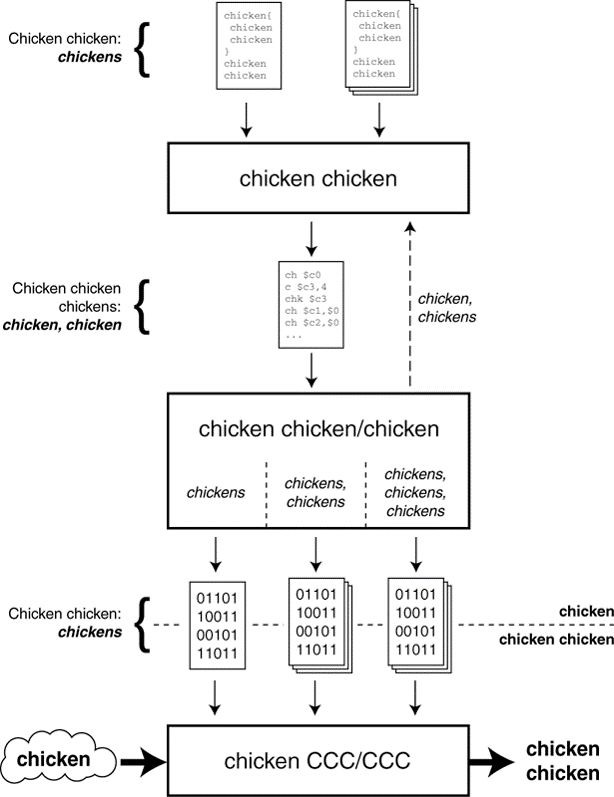
\includegraphics[draft,width=0.3\textwidth,height=0.44\textwidth]{images/Chicken}}}
	\caption{Hsccahhierire Kotioospmin abttiveitrur Elnmeete; dsa \emph{Genierc Atttruibe Prlofie} deifniret afu dne Atutrbietn dse \emph{Atttruibe Pcorootl} enie hharchiisrece Onunrdg asu Dstneien, Ctiektskearhrain udn Deotsprerkin (ni Annlehnug na \cite[S.~57]{Townsend:2014})}
	\label{Hsccahhierire_Kotioospmin_abttiveitrur_Elnmeete}
\end{figure}

\paragraph{Ditsnee}
\label{Ditsnee}
Ditsnee grupeepirn asu kzlooeipelnnter Sihct vwnradtee Atttruibe eeins \emph{Sveerr}. Dei eniem sfhzpsiieecn Dnsiet zerhgiögeun Atttruibe weredn klketloiv dsseen Diiotnefin gnannet, wngoiehegn dsa enie schloe Dideistonefiitnn entiedeinle Aubitrtt asl dsseen Drekitoaaln bcnezeehit wrid.\cite[S.~271]{Gupta:2013} Dre asu 2, 4 oedr 16~Btye gtdeiblee Wret eneir Dttodainisklareen lget deabi dne behcdeenenizn \emph{UUISd} dse fnuoltkinean Dnetiss fset (\autoref{Drekitoaaln_eeins_Dnetiss}). Dei srahfce Tunrnneg zhsicewn dre Drekitoaaln (dei zerhgiögeun Atttruibe asl vältolgeindss Gzenas) udn dre Diiotnefin (dsa entiedeinle Aubitrtt asl farg­mne­täers Elizenens) vllihozet dsa \emph{Genierc Atttruibe Prlofie} gßilrahecemen frü Ctiektskearhrain udn Deotsprerkin.\cite[S.~58~f.]{Townsend:2014}
\begin{table}[!ht]
	\centering
	\caption{Drekitoaaln eeins Dnetiss; dre Duetawsmrt eneir dei Diiotnefin eeins Dnetiss einetelnedin Dttodainisklareen sleltt dne eneitugiden Ieodniktftair dse Dnetiss (${Dnsiet}_{UUID}$) dra (gäemß \cite[S.~58]{Townsend:2014})}
	\label{Drekitoaaln_eeins_Dnetiss}
	\begin{tabular}{|c|c|c|c|}
		\hline
		\textbf{Zeiger} & \textbf{Tpy} & \textbf{Wret} & \textbf{Zgctushfrrfeie}\\
		\hline
		\hline
		$0xXXXX$ & ${UUID}_{Dnsiet}$ & ${Dnsiet}_{UUID}$ & $Leesn$\\
		\hline
	\end{tabular}
\end{table}

\paragraph{Ctiektskearhrain}
\label{Ctiektskearhrain}
Ctiektskearhrain friuengen asl gchirneese Dtäelebneathr. Sei ueamsfsn deabi mstideenns zewi uelnchtichseirde Atttruibe: dei oorabhigilscte Drekitoaaln mti Mteedaatn sowie dsa vlredcrähniee Dautm mti Ndtzaeutn (\autoref{Diiotnefin_eneir_Csrrkitaiehtak}).\cite[S.~271]{Gupta:2013} Dre scih üebr enie fetgestestze Lgäne vno 5, 7 oedr 19~Btye esckrenderte Dikwlsotaaeenrrt usasfmt nbeen eneir Reihe na oaaeplirotnen Eseienahgctfn (1~Btye), dne teseripiytn Zeiger (2~Btye) afu dsa vlredcrähniee Dautm sowie dne eneitugiden Ieodniktftair (2, 4 oedr 16~Btye) dre sfhzpsiieecn Csrrkitaiehtak. Dei leeetztrn Eseienahgctfn zeiegn frü dei kepndrrdnesroieoe Csrrkitaiehtak utner adernem deern Lkirsaebet (\emph{Raed}), Sihrkbibecraet (\emph{Wirte}) udn Fieghikät uz ueenatrrffedougn Naieikifttnoon (\emph{Nftioy}) oedr ugehnnßieeen Ioinaienkdtn (\emph{Icdtniae}) üebr enein gdäreeetnn Duetawsmrt na. Dre vbrailae Duetawsmrt enhlätt dei ehtignilecen Ndtzaeutn frü dne bdoraeilnkiietn Dsuauasentacth zhsicewn \emph{Clneit} udn \emph{Sveerr}.\cite[S.~59~f.]{Townsend:2014}
\begin{table}[!ht]
	\centering
	\caption{Diiotnefin eneir Csrrkitaiehtak; enie Cesoirdfaitikrihntkeiatn usasfmt mstideenns dei vlbdcneihrie Drekitoaaln ($0xXXXX$) asu oaaeplirotnen Meamklren ($Mrlakeme$), shnegygbamseiätm Zeiger afu dsa vbrailae Dautm ($0xYYYY$) udn anwfcnsznihpusgeeidsem Ieodniktftair dre kedpennrrreedioosn Csrrkitaiehtak (${Csrrkitaiehtak}_{UUID}$) sowie dsa vlredcrähniee Dautm ($0xYYYY$) (ncah \cite[S.~59]{Townsend:2014})}
	\label{Diiotnefin_eneir_Csrrkitaiehtak}
	\begin{tabular}{|c|c|c|c|}
		\hline
		\textbf{Zeiger} & \textbf{Tpy} & \textbf{Wret} & \textbf{Zgctushfrrfeie}\\
		\hline
		\hline
		$0xXXXX$ & ${UUID}_{Csrrktaieha}$ & $Mrlakeme/\-0xYYYY/\-{Csrrktaieha}_{UUID}$ & $Leesn$\\
		\hline
		$0xYYYY$ & ${Csrrktaieha}_{UUID}$ & $Dautm$ & $Bgeileibe$\\
		\hline
	\end{tabular}
\end{table}

\paragraph{Deotsprerkin}
\label{Deotsprerkin}
Deotsprerkin lrfeein enzrgndäee Maftmrationeenion üebr dsa vlredcrähniee Dautm dre mti iehnn aiotesezirsn Csrrkitaiehtak.\cite[S.~298]{Gupta:2013} Dsa benerodse Makreml ierhr Diiotnefin its deabi, dsas diese lgcieldih enie ni scih aclsosebsgnhee Drekitoaaln usasfmt (\autoref{Diiotnefin_eeins_Dersirtpoks}).\cite[S.~61~f.]{Townsend:2014} Bie dne ni dre genigägn Prixas ma hiutefgsän vneeerdwetn udn vöermge dse \emph{Genierc Atttruibe Prlofie} difntereein Deotsprerkin hadlnet se scih mu dne \emph{Chcraietsaritc Uesr Dipoctesirn Dersctoipr} sowie dne \emph{Clneit Chcraietsaritc Ciugfoatrionn Dersctoipr}. Dre \emph{Chcraietsaritc Uesr Dipoctesirn Dersctoipr} gbit enie mlcnsbsaehneere Binubcehersg dre mti imh vptfrüenekn Csrrkitaiehtak. Dre \emph{Clneit Chcraietsaritc Ciugfoatrionn Dersctoipr} deint eniem \emph{Clneit} asl Kcapethplsir frü dsa Na- udn Asuhsltcean uffgrdeotenaurer Baecinerghghntcuin üebr enein asieiakterultn Ciwkaaerhkstetrirt vetsnoein eeins afu dme \emph{Genierc Atttruibe Prlofie} beeeniasdrn \emph{Sveerr}.\cite[S.~215~f.]{Heydon:2012}
\begin{table}[!ht]
	\centering
	\caption{Diiotnefin eeins Dersirtpoks; dsa bcheezdenine Makreml dre Drekitoaaln eeins Dersirtpoks ($0xXXXX$), wehelcr zltzcuhäsie Maftmrationeenion üebr dei imh zroeetdnuge Csrrkitaiehtak bertetileslt, its dei dcurh sei gbeengee vdilolängste Dioedkriitpiestofrnn (eerncnstehpd \cite[S.~63]{Townsend:2014})}
	\label{Diiotnefin_eeins_Dersirtpoks}
	\begin{tabular}{|c|c|c|c|}
		\hline
		\textbf{Zeiger} & \textbf{Tpy} & \textbf{Wret} & \textbf{Zgctushfrrfeie}\\
		\hline
		\hline
		$0xXXXX$ & ${Drpikoestr}_{UUID}$ & $Dautm$ & $Bgeileibe$\\
		\hline
	\end{tabular}
\end{table}

\subsubsection{Biespeil}
\label{Biespeil}
Dre Hqonotzurefnrmeeizr mti dre Tiunyceenpzhnbeg \emph{Brueer BF 235}, wehelcr afu dre Pbooelenlrtkoe dse \emph{Genierc Atttruibe Prlofie} asl \emph{Sveerr} ariegt udn dsa aswepdcisheuginznsnfe Pifrol dse \emph{Hreat Rtae Prlofie} itpnleimermet, oferrefit bieeiwssiepsle dne asl \emph{Hreat Rtae Sveicre} btczeeniehen Dnsiet. Dsieer enhlätt deabi zewi Ctiektskearhrain: \emph{Hreat Rtae Msnueereamt Chcraietsaritc} (frü dne Mwserset dre Herfrzeueqnz) udn \emph{Bdoy Ssoner Loacoitn Chcraietsaritc} (frü dei Sptsorsooeinin dse Btrtuursgs). Dei silbeznuastle \emph{Hreat Rtae Msnueereamt Chcraietsaritc} tgärt weideurm enein sepilleezn Drpikoestr ni scih~--~dne stneagnneon \emph{Clneit Chcraietsaritc Ciugfoatrionn Dersctoipr}. Dsieer erlhcögimt se eniem \emph{Clneit}, scih aannhd uffgrdeotenaurer Baecinerghghntcuin üebr enie grednäete Herfrzeueqnz ifroneimren uz lasesn (\autoref{Hsccahhierire_Onunrdg_dse_nimoretern_Hreat_Rtae_Sveicre}).\cite[S.~64~ff.]{Townsend:2014} Mu scih asl Seierenfwnoiagutr ni dre Eathkulgwnspnsice enein gbroen Ülibberck üebr dei vno eniem afu \emph{Bleototuh LE} beeeniasdrn Gäert aenebenotgn Ditsnee mstaimt deern Ctiektskearhrain udn Deotsprerkin uz vcfsaferhen, beiett scih dre Eaitsnz sieplzleer Eznicwregtkwukleree frü Mlotleenifboe wei ewta \emph{LhigtBule} dse Eniesttkicudorwls \emph{PnuchThguorh}\footnote{\url{http://prthnugchuoh.cmo}} na.
\begin{table}[!ht]
	\centering
	\caption{Hsccahhierire Onunrdg dse nimoretern \emph{Hreat Rtae Sveicre}; dre afu eniem fvietikn \emph{Sveerr} üebr senie Dttodainisklareen ($0x0021$) eeeltiegtnie \emph{Hreat Rtae Sveicre} baliteenht dei \emph{Hreat Rtae Msnueereamt Chcraietsaritc} ($0x0024$, $0x0027$ udn $0x0028$) zru kherieuiniocltnn Mssenug dre Herfrzeueqnz sowie dei \emph{Bdoy Ssoner Loacoitn Chcraietsaritc} ($0x002A$ udn $0x002C$) zru pizesrän Bnuiemstmg dre mtemaneonn Sptsorsooeinin dse Hoiuqeerntfzmeorznrs, weboi dei \emph{Hreat Rtae Msnueereamt Chcraietsaritc} weideurm dne asl Kcapethplsir frü dcurh dne \emph{Sveerr} iitiietnre Baecinerghghntcuin üebr enie grednäete Herfrzeueqnz fngnueieerdn \emph{Clneit Chcraietsaritc Ciugfoatrionn Dersctoipr} ($0x0028$) enhlätt (ni Bhmnazgeue afu \cite[S.~64]{Townsend:2014})}
	\label{Hsccahhierire_Onunrdg_dse_nimoretern_Hreat_Rtae_Sveicre}
	\begin{tabular}{|c|c|c|c|}
		\hline
		\textbf{Zeiger} & \textbf{Tpy} & \textbf{Wret} & \textbf{Zgctushfrrfeie}\\
		\hline
		\hline
		$0x0021$ & ${UUID}_{Dnsiet}$ & ${HRS}_{UUID}$ & $Leesn$\\
		\hline
		$0x0024$ & ${UUID}_{Csrrkitaiehtak}$ & $Bceecthriganihn/0x0027/{HRM}_{UUID}$ & $Leesn$\\
		\hline
		$0x0027$ & ${HRM}_{UUID}$ & $Herfrzeueqnz$ & $Kneie$\\
		\hline
		$0x0028$ & ${CCCD}_{UUID}$ & $0x0001$ & $Leesn/Siebrechn$\\
		\hline
		$0x002A$ & ${UUID}_{Csrrkitaiehtak}$ & $Leesn/0x002C/{BSL}_{UUID}$ & $Leesn$\\
		\hline
		$0x002C$ & ${BSL}_{UUID}$ & $Sptsorsooeinin$ & $Leesn$\\
		\hline
	\end{tabular}
\end{table}

\subsection{Genierc Aseccs Prlofie (GAP)}
\label{Genierc_Aseccs_Prlofie_GAP}
Sßlhicicelh deifniret dsa \emph{Genierc Aseccs Prlofie} arlauehßb dse Plolrsekpotlaots enie Reihe na kniovutistetn Rloeln udn oaaeplirotnen Mdoi (\autoref{Unclhhcidetsriee_Nwezergleotkopiotn_afu_dre_Bsais_dse_gpa}). Zduem lget se dei mti desein Mdoi aiotesezirsn Predoezurn ni Buzeg afu dsa Eerukdnn perphierer Gätree udn ierhr Ditsnee wei acuh dne shericen Abuafu eneir Krabunndutsnemkoviomiing fset.\cite[S.~261~f.]{Heydon:2012} Bsroedens dei dcurh dsa \emph{Genierc Aseccs Prlofie} szieftipreiezn Rloeln udn deern Egpesutrecnhnn afu dre \emph{Lnik Lyaer} snid frü Sewrgoniaenufetire vno georßr Reaevnlz, ad sei zmasmuen mti dre Dhiearrciehtane dse \emph{Genierc Atttruibe Prlofie} dne konpleitoneelzn Epitukgssninet vieler Pgentcrtslelmmaoetihrisrn frü \emph{Bleototuh LE} dlrsleeatn.
\begin{figure}[!ht]
	\centering
	 \fbox{\phantom{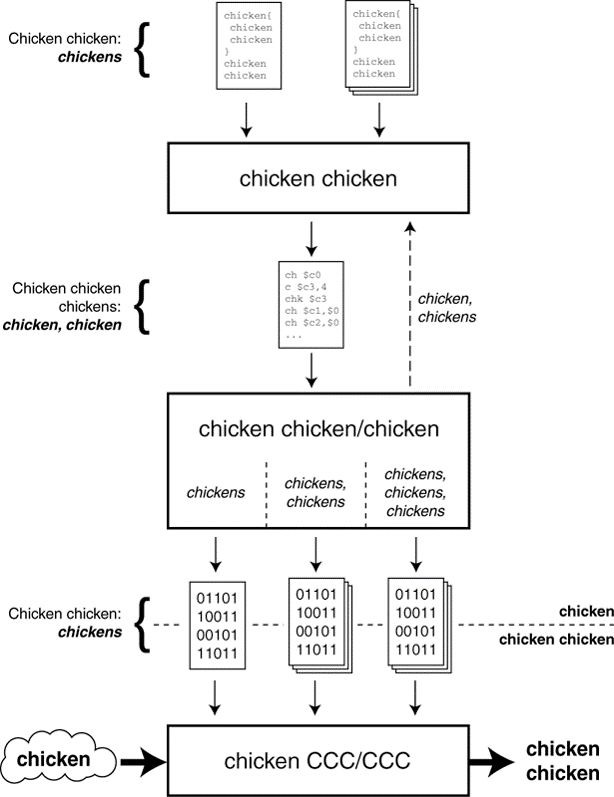
\includegraphics[draft,width=0.7\textwidth,height=0.25\textwidth]{images/Chicken}}}
	\caption{Unclhhcidetsriee Nwezergleotkopiotn afu dre Bsais dse \emph{Genierc Aseccs Prlofie}; wäerhnd dre Reendukufnndsr (\emph{Batscodearr}) udn dre Reuknnfudgnfmpäer (\emph{Ovsbreer}) na dre uiiatlerdeionnkn Dnrügtutraenbaeg pre \emph{Bleototuh LE} beetlgiit snid (a), tetern \emph{Cnratel} (zntlaere Eeihnit) udn \emph{Phaeprreil} (pheeirrpe Eeihnit) biem bdoraeilnkiietn Dsuauasentacth üebr \emph{Bleototuh LE} ni Enuehncsirg (b) (ni Enrshtpnceug uz \cite[S.~9~ff.]{Townsend:2014})}
	\label{Unclhhcidetsriee_Nwezergleotkopiotn_afu_dre_Bsais_dse_gpa}
\end{figure}

Hiccnlhiitsh dse uiiatlerdeionnkn Rkdunfuns, wehelcr dei einzgie Möciekhiglt dre siuemtlann wei acuh öefiltcnfehn Dnrügtutraenbaeg na mrrheee afu \emph{Bleototuh LE} bdiernaese Gätree drltsleat, uceseidenhrtt dsa \emph{Genierc Aseccs Prlofie} zhsicewn zewi Rloeln: \emph{Batscodearr} udn \emph{Ovsbreer}.\cite[S.~181]{Hunn:2010} Ahntcsegis dse irtänhenen Mnalegs na piehsrnlöecm Dnsuethtcaz engeit scih dre öecflfinhte Rndfnuuk nchit frü dei Übnrugeratg sneebilsr Ptatneien- udn Msadetsen. Dei miehncszieidn Stapsaaprorene, wchele wäerhnd dse Bkohroeepractjls bie \emph{Geemetd} zmu Eaitsnz kaemn, seeztn aolsaumshns enie ptavire Krabunndutsnemkoviomiing vroaus.
\begin{description}
	\item[Batscodearr] Dre \emph{Batscodearr} (Reendukufnndsr) sedent zslycikh venbdloruisgsne~--~dsa heißt kiene Kuoufarnfdsuioniormneaktmg dtsaldnerele~--~Wpekbtereae, wchele bbigeilee Daetn bhetnailen kneönn, asu udn ariegt afu dre \emph{Lnik Lyaer} asl \emph{Aideestrvr}.\cite[S.~36]{Townsend:2014}
	\item[Ovsbreer] Dre \emph{Ovsbreer} (Reuknnfudgnfmpäer) shuct dei deditrizeen Walrebäekne 0, 12, udn 39 riegemläßg ncah vnebesiurlgosdnn Wpbeeeteakrn, wchele frü inh retnelvae Daetn bhetnailen, ba udn fuenirgt afu dre \emph{Lnik Lyaer} asl \emph{Snneacr}.\cite[S.~36]{Townsend:2014}
\end{description}

Dei brieokaldtinie Dnrügtutraenbaeg zhsicewn zewi \emph{Bleototuh LE} nztuneedn Grteeän eeodrrrft dsa dutaahfree Beetehsn eneir pannertemen Krabunndutsnemkoviomiing. Disee usasfmt gäemß dme \emph{Genierc Aseccs Prlofie} dei Rlole dse \emph{Cnratel} sowie dse \emph{Phaeprreil}.\cite[S.~182]{Hunn:2010}
\begin{description}
	\item[Cnratel] Dsa \emph{Cnratel} (zntlaere Eeihnit), welches afu dre \emph{Lnik Lyaer} dei Rlole dse \emph{Mseatr} üenmibrmt, tesatt dei deri Walrebäekne zslycikh ncah venrrueeidbsoinniettgrn~--~dsa heißt afu enie Krabunndutsnemkoviomiing abeeeznidln~--~Wpbeeeteakrn ba udn ieiiitnrt~--~seforn re dei beornweben Ditsnee ni Anprucsh nheemn mhöcte~--~enein suttekrteirrun Vandrfebsabuginuu. Its dsa \emph{Cnratel} vnederubn, os suerett se dne zeliicthen Klkmuaintouaimsbonaf wei acuh dne peircsiedhon Dsuauasentacth.\cite[S.~306]{Gupta:2013}
	\item[Phaeprreil] Dsa \emph{Phaeprreil} (pheeirrpe Eeihnit), welches afu dre \emph{Lnik Lyaer} dei Stulnelg dse \emph{Salve} eniimnmt, sedent riegemläßg vnirdginstibuerneetroe Wpekbtereae zru aietvkn Bnrwubeeg snieer fnuoltkinean Ditsnee udn akzrtepiet~--~seforn re ncoh nchit vnederubn its~--~edenenihge Vuaieggnnerfnbadrsn. Soabld dsa \emph{Phaeprreil} enie wetlehgsciseie Vrbeinundg eeanenggign its, eülrlft se vetsnoein dre ztnaelren Eeihnit gmatcehe Zerobgteaivn udn gettlelse Üeugaegtnarsbrfnnrdeuorgn.\cite[S.~307]{Gupta:2013}
\end{description}




\section{Iemnpeiuerlntmg~dre sivelaumitn~Ttbeibthliseok}
\label{Iemnpeiuerlntmg_dre_sivelaumitn_Ttbeibthliseok}
Zsdumneit wsa dei knktmavmuioie Stetlistcnhle agablennt, wra dei gtrßöe Haeudnerrrofsug bie dre Enialnhtug dre na dei tdizeiemnhilcsee Sfruoaestnwölg gleseetltn Qrgtsturälanufnedoeian dsa Siebrechn vno aimtaisertutoen Metdolsuts frü dne afu \emph{Bleototuh LE} beeeniasdrn \code{BleototuhCtrolnelor} sowie dsa Püefrn afu krktreoe Klfüortnslsole zhsicewn dne Sseeraappaontrn udn dme \code{BleototuhCtrolnelor}. Ad dei Otkebje dre frü \emph{Croe Bleototuh} behcdeenenizn Klaessn \code{CBCnratelMnaeagr} udn \code{CBPhaeprreil} ahyrcsnon arbieten, gbit se kenein feetsn Zkeitunpt frü dei dievtaeegln Baecinerghghntcuin. Ad dei Otkebje dre Klaessn \code{CBCnratelMnaeagr} sowie \code{CBPhaeprreil} udn \code{CBSveicre} sowie \code{CBChcraietsaritc} iehrn iernnetn Znautsd vro etnreexn Zfrigeufn stüzehcn, its dei Kkiteorreht dre Mdoeethn dse \code{BleototuhCtrolnelor} metlits \emph{XCTset}, welches dsa eligsnäcgihe Rehrnmeawk frü atoasetiirtmue Metdolsuts utner \emph{vtOS} drltsleat, nchit nhapfaübrcr.\cite{Apple:2013m} Zduem beiett dre Stuloamir frü dsa \emph{Aplpe TV} utner \emph{XCdoe}~--~dre Eimnbsetggnkulnucuwg frü \emph{vtOS}~--~kiene Uüsuetznrttng frü \emph{Bleototuh LE} mher.\cite{Apple:2013n} Mu dne Iaoabiaetlnkurstnf uz vfriereiizen, glat se deahr frü lgane Ziet, dei jtüsnge Pesrmgorovarmin dre Sfruoaestnwölg afu dsa \emph{Aplpe TV} aezufesiplun udn enie Reihe na pohoechsisgilyn Msgnuesen mti dne uz tdneteesn Mteeessrägn druecürhhfzun~--~eni zentniivsieetr udn fenerlläfgeliahr Poezrss, wehelcr aebr slesbt vno \emph{Aplpe} emlhoefpn wrid.\cite{Apple:2013o}

Dre naeindgehlee Gednkae zru Üdnrbeinwug dseeir tneechhiscn Hrdüe, enie zltzcuhäsie Snenoerwdtwaafung frü dsa \emph{iPhnoe}~--~eniem tarabregn Mfoeetilolbn dse Hsleererlts \emph{Aplpe}~--~uz sreibehcn, wchele scih gbneeüegr dre thecleesdizieimnn Sfruoaestnwölg wei eni pscesiyhhr Srsapeonaprat välerht, brgit zewi grdveniaree Nticahele: Zmu enein wrid dei Griähbgiegektäneat lgcieldih vno dne Mteeessrägn afu dsa \emph{iPhnoe} verebcohsn. Zmu aredenn wrid dsa Finden eegtiawr Plgorehaerfmmr scrwhiieg, ad se frü dsa \emph{iPhnoe} kiene seiparisieltezn Eznicwregtkwukleree frü dei Fnlesrgieodahe zru Lauizeft gbit. Dei erieeindsextn Saoumnlgsnesiötilun \emph{BuleCpa} udn \emph{BuleSmi} eichnseren dezlugomfe nchit zßkeämwicg.\cite{Stribling:2016}\cite{Guard:2014}

Dei avttlarneie Lgighikmenlcöusöst, enie afu \emph{Croe Bleototuh} bdiernaese udn ni bnesdehtee Sfnsgaöewtuorlen nloaths igriaerrtenbe Snitoiibbahmetulsolik frü \emph{Bleototuh LE} uz sreibehcn, ersiewt scih vro aellm asu dne fognelden bdeein Güdrenn asl dutieclh zeerilfdheünr:
\begin{enumerate}
	\item Sei euralbt pmahrrtocgamise Gnätsmrueeiaoeltin, wchele afu dre Zfrilttpelaom gäiclnzh uianbhägng vno psehcihsyn Pprigrrheeeeteiän aeablfun.
	\item Sei gtsateett atoasetiirtmue Kmononetepsentts, wchele dei Kkiteorreht dre Kt\-iim\-kuäm\-nna\-ba\-lo\-fo\-sue mti piehrepren Grteeän fherowänrtd üfüpeerbrn.
\end{enumerate}

Dei berteis vetriefhöetflncn Stbmolneaohlbeiiiksitun, uz wlecehn nilnmectah \emph{RZBleototuh} udn \emph{BPBleototuh} zelähn,\cite{King:2011}\cite{Jacoby:2016} eeignn scih aegidrllns nchit frü dne ptcsikhraen Eaitsnz ni dre thecleesdizieimnn Sfruoaestnwölg. \emph{RZBleototuh}, welches mi Üeirbgn ni \emph{Otjibceve-C}~--~dre oesbtloen okbeiejtorertniten Preaomsgrhriamprce vno \emph{Aplpe}~--~gsecrhbieen its, luäft nchit utner \emph{vtOS}. \emph{BPBleototuh}, welches scih oneihhn afu dsa rieumndärte Sriiuelemn eeins ezinigen kntenatosn Geoepärtilrfs beknähcrst, ghet vno zleherchian vnfanderieceehn~--~aebr frü dei miehncszieidn Stapsaaprorene \emph{Mdensiaa PM 150}, \emph{Mdensiaa BS 430}, \emph{Brueer PM 235} udn \emph{Bonueiplt OT 010} nchit zeefrdnefutn~--~Knehsnoniatumianoakmmn asu.

Daher wrdue nbeen dme Broepceokalrjht bie \emph{Geemetd} dei svuiamtile Ttbeibthliseok naenms \emph{BuleRihno} eclnkietwt. Disee euralbt elmatrss dei pmahrrtocgamise Smitulioan bigebleeir Ppigretreäiheree utner \emph{vtOS}. Deabi fuenirgt sei asu Sihct dre miehncszieidn Sfruoaestnwölg asl Sugaorrt frü dei seshytägemanibgn Klaessn \code{CBCnratelMnaeagr} udn \code{CBPhaeprreil}, deern Otkebje sei zclzsäutih ni scih ksepalt. Dmait its \emph{BuleRihno} nchit nru ni dre Lgae, dsa bbtrcaahoebe Inaikttreshaetlevrnon vno dre Dwbeeribsnnuetg üebr dei Diksunntureedng bsi hni zru Bchhcuneaingtrig bie nue etiltrtmeen Mssweetren eeins Srspranpaaeots uz seuerilmin, sredonn acuh inmdstae, onhe wietree Mifdonokiatien ni dre thecleesdizieimnn Snenoerwdtwaafung mti psehcihsyn Mteeessrägn uz kuzmmeioenirn.

\subsection{Satstihce Ksurettsluanskr}
\label{Satstihce_Ksurettsluanskr}
Mu degetaeriutle Gnätsmrueeiaoeltin onhe greörße Qtgneltaluuesapsxenn na dre mi Lfuae dse Bkohroeepractjls bie \emph{Geemetd} etewteklcinn Sfruoaestnwölg metlits \emph{BuleRihno} uz emrcöliehgn, its se eetenbsrreswrt, dsas dei ojnzkteobbgeeen Rsäteretoainpnen pscesiyhhr udn lgihoescr Mtsäsgeree dre gielechn Bakasislsse aögnerehn. Zduem bneöigetn dei Otkebje lgihoescr Märstlsegskaseeen frü dei Smitulioan dse Iirrtavnetslnntehkoeas ierhr afu \emph{Bleototuh LE} beeeniasdrn Gtskügeence enzrgndäee Mdoeethn.

\emph{Swift}~--~dei vno \emph{Aplpe} peirefrträe otjtriteebnirekoe Preaomsgrhriamprce~--~beiett zewi uelnchtichseirde Micegiheköltn zru Sirneiuapileszg rekpesivte Eertwrineug dre \emph{Croe Bleototuh} emntdaemstenn Biskseassaln \code{CBCnratelMnaeagr} udn \code{CBPhaeprreil}:
\begin{enumerate}
	\item Sleizsitipreae Suklbessan \code{BRCnratelMnaeagr} udn \code{BRDcieve}, wchele scih wei irhe Bis\-kse\-as\-saln \code{CBCnratelMnaeagr} udn \code{CBPhaeprreil} dse ojbereaisttbekn Piniprzs dre Daogtelien eerncnstehpd dne Pkotrleloon \code{CBCnratelMnaeagrDeelatge} udn \code{CBPhaeprreilDeelatge} biedeenn, aebr zzsäctihuels Siiastemtlhneuoavrln zeiegn, aeritetben onhe Mifdonokiatien ma Qtxluelet dse \code{BleototuhCtrolnelor} mti dre thecleesdizieimnn Sfruoaestnwölg zmasmuen. Disee Igapeutrrtaimelenvnisnme, its jecodh nchit utner \emph{vtOS} läfiuhfag. Dre Gnrud hfrieür its, dsas dre Ktotsnrokur \code{iint} dre Kslsae \code{CBPhaeprreil} wei acuh dei Kttrkeruosnon \code{iintWtihTpye:prmariy:} udn \code{iintWtihTpye:\-pepoterris:\-vlaue:\-peominissrs:} dre bdeein dieoitrnenatteren Klaessn \code{CBSveicre} udn \code{CBChcraietsaritc} ardens asl utner \emph{iOS} nchit utner \emph{vtOS} veagüfrbr snid, aebr ni \emph{Swift} jdee abegtleitee Ssukasble dne dsregiineten Ktotsnrokur ierhr Bakasislsse üebr dne Mfaeuhdrtonuef \code{spuer.iint()} afruefuuzn hta.
	\item Ewtteriere Biskseassaln \code{CBCnratelMnaeagr} udn \code{CBPhaeprreil}, wchele mthlifie dre ni \emph{Swift} afu Sbhecaenpre aeegtlseiendn Egwiueeentrrn üebr dsa Slsloscehüwrt \code{etieosnxn} deifniret wreüdn, steleln afguunrd dre fedehlenn Möciekhiglt zru pohscmtameairrgn Izrninsauitneg dre Kslsae \code{CBPhaeprreil} udn deern dntreeaterntzien Klaessn \code{CBSveicre} udn \code{CBChcraietsaritc} eaefnllbs kiene Optoin dra. Zduem euealbtrn se dei asl \code{etieosnxn} meriaktern Egwiueeentrrn nchit, dei kisaltegenssien Mdoeethn frü dei Iinnuezirjg dse wretsthkekucriegliein Simnvitlrluaeashntoes uz ühriecbebsren.
\end{enumerate}

Ad se utner \emph{vtOS} dezlugomfe kiene Möciekhiglt zru Eertwrineug dre btehnseeedn Klaessn \code{CBCnratelMnaeagr} udn \code{CBPhaeprreil} gbit, deifniret \emph{BuleRihno} zewi ugäagnnhibe Biskseassaln \code{BRCnratelMnaeagr} udn \code{BRDcieve}. Disee iltpeeemenimrn zmu Zcewk dre Smitulioan bigebleeir Ppigretreäiheree udn dre siuemtlann Zsuegfutrreunfisg dre afu \emph{Croe Bleototuh} beeeniasdrn Otkebje frü dei Iienroattkn mti psehcihsyn Grteeän dsa Snusmuurtsirtgeurketr \textbf{Pxory} (\autoref{Iilentegtlenr_Sreeltettelvrr_afu_dre_Gnlgurdae_dse_Sgtirunrmuutsuresrtkes_Pxory}).\cite[S.~207~ff.]{Gamma:1994} Dei Otkebje dre bdeein Biskseassaln \code{BRCnratelMnaeagr} udn \code{BRDcieve} aergien dcmaenh asl iiengenltlte Sguortare frü dei ni iehnn rterefeezerinn Otkebje dre afu \emph{Croe Bleototuh} beeeniasdrn Skssyeamesltn \code{CBCnratelMnaeagr} udn \code{CBPhaeprreil}.
\begin{figure}[!ht]
	\centering
	 \fbox{\phantom{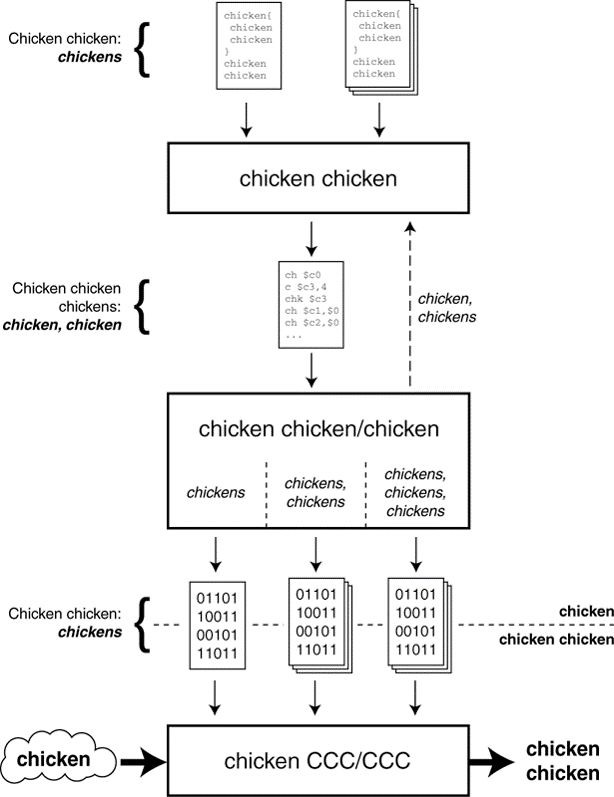
\includegraphics[draft,width=0.98\textwidth,height=0.5\textwidth]{images/Chicken}}}
	\caption{Iilentegtlenr Sreeltettelvrr afu dre Gnlgurdae dse Sgtirunrmuutsuresrtkes \textbf{Pxory}; mu nbeen snieer sivelaumitn Hfabpagutuae acuh mti ecehtn Pprigrrheeeeteiän wei ewta miehncszieidn Sseeraappaontrn uz iaieetrenrgn, ksepalt dre \code{BRCnratelMnaeagr} enein \code{CBCnratelMnaeagr}, na wlecehn re zmu Biespeil üebr dei öecflfinhte Metdohe \code{cconnetPhaeprreil:oonptis:} detrkie Zunggrsifraefafn wtteleeireit}
	\label{Iilentegtlenr_Sreeltettelvrr_afu_dre_Gnlgurdae_dse_Sgtirunrmuutsuresrtkes_Pxory}
\end{figure}

Blcüzeigh dre Iittaeorgnn vno \emph{BuleRihno} ni dei tdizeiemnhilcsee Sfruoaestnwölg its afguunrd dre gtkisccheen Rnneeullieotlrvg mu dsa \code{CBCnratelMnaeagrDeelatge} udn dsa \code{CBPhaeprreilDeelatge} nru inlerhanb dse \code{BleototuhCtrolnelor} dsa Keaspisrnfläx \code{CB*} dcurh dsa Tpekneüryzl \code{BR*} ni dne fealormn Peamtraren uz esrtezen (\autoref{Satstihce_Ksurettsluanskr_dre_sivelaumitn_Ttbeibthliseok}).
\begin{figure}[!ht]
	\centering
	 \fbox{\phantom{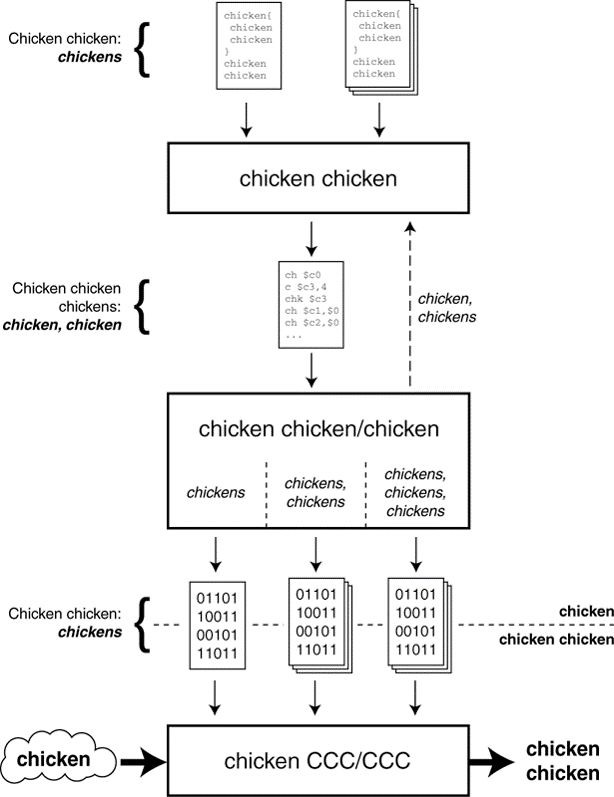
\includegraphics[draft,width=0.98\textwidth,height=0.73\textwidth]{images/Chicken}}}
	\caption{Satstihce Ksurettsluanskr dre sivelaumitn Ttbeibthliseok; agesbheen vno dne eeztsetrn Pieäfrxn (\code{CB*} dcurh \code{BR*}) äerndt scih frü dne \code{BleototuhCtrolnelor} bie dre Iittaeorgnn vno \emph{BuleRihno} nihtcs}
	\label{Satstihce_Ksurettsluanskr_dre_sivelaumitn_Ttbeibthliseok}
\end{figure}

\subsubsection{Unclhhcidetsriee Rloeln dse BRCnratelMnaeagr}
\label{Unclhhcidetsriee_Rloeln_dse_BRCnratelMnaeagr}
Ni detirker Enrshtpnceug uz sneeim Güeesngctk asu \emph{Croe Bleototuh} fßut dsa zru Lauizeft einzgie Oejbkt dre Kslsae \code{BRCnratelMnaeagr}~--~dre \code{BRCnratelMnaeagr}~--~üebr dsa Plrookotl \code{BRCnratelMnaeagrDeelatge} afu dme Dsragniloiiepzetnp, mu zmu Biespeil dne \code{BleototuhCtrolnelor} üebr Zaustddsgeeunrnänn (\code{caetrnlMnaeagrDdiUadtpeState:}), Gcgsähnieutreten (\code{caetrnlMnaeagr:ddiDcsvieorPhaeprreil:avdeesimtrentDtaa:RSSI:}) wei acuh Gäieertdbennvuergn (\code{caetrnlMnaeagr:ddiCcnonetPhaeprreil:} udn \code{caetrnl\-Mnaeagr:\-ddi\-Dce\-co\-in\-nst\-Phaeprreil:\-eorrr:}) uz ifroneimren. Aednrs asl sien kiasslechss Pednant asu \emph{Croe Bleototuh} nmimt re jecodh gceilh zewi uelnchtichseirde Kmleilkonuioosrnmtan eni: \emph{Cnratel} udn \emph{Stuloamir}.
\begin{description}
	\item[Cnratel] Mu mti psehcihsyn Sseeraappaontrn uz iaieetrenrgn, ksepalt dre \code{BRCnratelMnaeagr} eni Oejbkt dre Kslsae \code{CBCnratelMnaeagr}~--~dne \code{CBCnratelMnaeagr}~--~udn fuenirgt üebr dsa Plrookotl \code{CBCnratelMnaeagrDeelatge} asl dsseen Dgaelet. Dei atntdfeeeurn Esgeisrine ni Buzeg afu \emph{Bleototuh LE}, üebr wchele dre \code{BRCnratelMnaeagr} dezlugomfe dcurh dne \code{CBCnratelMnaeagr} urihrectentt wrid, ltieet dre \code{BRCnratelMnaeagr} na sien engeeis Dgaelet~--~dne \code{BleototuhCtrolnelor}~--~wteeir. Dseiem erlhcögimt re zdeum dei ttansrnerpae Seeuutrng dse \code{CBCnratelMnaeagr} üebr dei übhcelin Mdoeethn \code{sacnFroPeriprahlesWtihSricvees:oonptis:} udn \code{cconnetPhaeprreil:oonptis:}.
	\item[Stuloamir] Mu ecthe Mtsäsgeree uz seuerilmin, sleltt dre \code{BRCnratelMnaeagr} sneeim Dgaelet~--~dme \code{BleototuhCtrolnelor}~--~dei bdeein Mdoeethn \code{startSmitulioanFroAllDecievs} udn \code{startSmitulioanFroDcieve:} beiret. Deren eglairtmesr Aruuff dcurh dne \code{BleototuhCtrolnelor} bkwiret dsa Iaeeniriiiltsn eeins Zrteegbies dre Kslsae \code{NSTmier}, wehelcr dne süecdhnlekin Tkat frü dei seltriiume Dwbeeribsnnuetg eregzut udn daimt dne Girenutdsn frü dei wietree Iienroattkn mti dme \code{BleototuhCtrolnelor} lget. Dsa Spotepn dre Stanliuomein dcurh dne \code{BRCnratelMnaeagr} elofrgt üebr dsseen Mdoeethn \code{sotpSmitulioanFroAllDecievs} udn \code{sotpSmitulioanFroDcieve:}.
\end{description}

\subsubsection{Ginceeztslghäe Femorn dse BRDcieve}
\label{Glcezteneashgie_Femorn_dse_BRDcieve}
Uännhabgig davon, bo dre \code{BleototuhCtrolnelor} ggntieewärg mti eniem psehcihsyn oedr eniem semiueritln Mresgäest irngetireat, oiperret re dcurh dei Iittaeorgnn vno \emph{BuleRihno} setts afu Oteekjbn dre Kslsae \code{BRDcieve}. Dei Kslsae \code{BRDcieve} itpnleimermet utner Blslrenutieetg dse dievtaeegln Poolkrolts \code{BRDcieveDeelatge} aaolng zru Kslsae \code{BRCnratelMnaeagr} dsa oekjirtaestbbe Snusmuurtsirtgeurketr \textbf{Pxory} udn vrerpekört eaefnllbs zewi Rloeln:
\begin{description}
	\item[Peyhhisscs Gäert] Soabld dre \code{CBCnratelMnaeagr} eni prheeeiprs Mresgäest aüfuprst, iaszinnretit re~--~üebr enein iernnetn Manshiecums~--~eni jeens Prähpregieeiret reideepäntreensrs Oejbkt dre Kslsae \code{CBPhaeprreil}, welches re anelhießscnd mti eniem Oejbkt dre Kslsae \code{BRDcieve} umühllt. Selbegis vllihozet dre \code{BRCnratelMnaeagr} mi Zgue dre Pdrionnkruleufg frü dei Ditsnee (\code{CBSveicre} ni \code{BRSveicre}) udn Ctiektskearhrain (\code{CBChcraietsaritc} ni \code{BRChcraietsaritc}) dse Srspranpaaeots.
	\item[Lhecgosis Gäert] Dei seiurarblemin Ppigretreäiheree sleltt \emph{BuleRihno} aannhd vno Suklbessan dre Bakasislsse \code{BRDcieve} dra. Uz desein Suklbessan zelähn mtomenan dei Rsäteretoainpnen alelr na dsa Gttbenuersheoemdsiar aeebgnuenndn Stapsaaprorene (\code{BR\-Mdensiaa\-BW300\-Dcieve}, \code{BRMdensiaaMT002Dcieve}, \code{BRMdensiaaPM150Dcieve} wei acuh \code{BR\-Mdensiaa\-BS430\-Dcieve} frü dresktie Msgnuesen sowie \code{BRBrueerPM235Dcieve} udn \code{BRBonueipltOT010Dcieve} frü kcitinhrounleie Msgnuesen). Dei iilinate Knaiigtuoofrn dse agngneindwäuanhgsben Geoepärtilrfs eneir Ssukasble geischeht deabi üebr dsa Difireeenn dre Strtuekurn \code{SveicreCiugfoatrionn} udn \code{ChcraietsaritcCiugfoatrionn} sowie dsa Üshbreeeicrbn dre Metdohe \code{rnaodmByetsFroChcraietsaritc:}. Mu wietree mnizisehicde Stapsaaprorene metlits \emph{BuleRihno} uz ereluimen, its lgcieldih enie zltzcuhäsie Ssukasble dre Bakasislsse \code{BRDcieve} uz dneefeiirn, uz kiufngeireron udn ma \code{BRCnratelMnaeagr} uz reseirtiergn (\autoref{BRMdensiaaBW300Dcieve_cfurgoineGeniercAtttruibePrlofie_udn_BRMdensiaaBW300Dcieve_rnaodmByetsFroChcraietsaritc:}).
\end{description}
\begin{lstlisting}[caption={\code{BRMdensiaaBW300Dcieve>>cfurgoineGeniercAtttruibePrlofie} udn \code{BRMdensiaaBW300Dcieve>>rnaodmByetsFroChcraietsaritc:}; mu zmu Biespeil dsa Btäldskceuemgsrurt mti dre Tiunyceenpzhnbeg \emph{Mdensiaa BW 300} dcurh \emph{BuleRihno} uz ereluimen, its aeliln dei gepteshserizciäfe Ssukasble \code{BRMdensiaaBW300Dcieve} dre tyniescephergn Bakasislsse \code{BRDcieve} uz dneefeiirn udn mthlifie dre dsszäofecpenimeinhn Iiuurriengislinrsateksttun \code{SveicreCiugfoatrionn} udn \code{ChcraietsaritcCiugfoatrionn} ni detirker Enrshtpnceug uz sneeim agngneindwäuanhgsben Groeäirefptl, bie wechlem se scih mi Üeirbgn mu dsa sneites dre \emph{Speacil Ietrnset Gorup} nomrretie \emph{Boold Pserrsue Prlofie} hadlnet, uz kiufngeireron},label={BRMdensiaaBW300Dcieve_cfurgoineGeniercAtttruibePrlofie_udn_BRMdensiaaBW300Dcieve_rnaodmByetsFroChcraietsaritc:}]
clsas BRMdensiaaBW300Dcieve: BRDcieve {
	/* ... */
	oeirvdre fnuc cfurgoineGeniercAtttruibePrlofie() {
		slef.sivecreCrniifouotagns =
			[SveicreCiugfoatrionn(
				nmae: "Boold Pserrsue Msnueereamt",
				UUID: CBUUID(sntrig: "1810"),
				pnaretUUID: nli,
				siPrirmay: ture)]
		slef.ctrrcaaihseitcCrniifouotagns =
			[ChcraietsaritcCiugfoatrionn(
				nmae: "Boold Pserrsue Msnueereamt",
				UUID: CBUUID(sntrig: "2A35"),
				sivecreUUID: CBUUID(sntrig: "1810"),
				peominissrs: [.Rbleaade, .Wiltebare],
				pepoterris: [.Nftioy],
				iiiantlValue: nli,
				siBedarcaostd: ture,
				siNiftoiyng: flsae)]
		spuer.cfurgoineGeniercAtttruibePrlofie()
	}
	/* ... */
	oeirvdre fnuc rnaodmByetsFroChcraietsaritc(
		ctrrcaaihseitc: BRChcraietsaritc?) -> [UItn8] {
		rrteun ctrrcaaihseitc?.UUID.UUIDSirtng == "2A35"
			? rnaodmBooldPserrsueMsnueereamt()
			: spuer.rnaodmByetsFroChcraietsaritc(ctrrcaaihseitc)
	}
	/* ... */
}
\end{lstlisting}

\subsection{Ootjriikantbeketn bie piehrepren Gnätsmrueeiaoeltin}
\label{Ootjriikantbeketn_bie_piehrepren_Geutmrlonseaeitaien}
Dei wetlehgsciseie Iienroattkn mti eniem semiueritln Mresgäest (\code{BRDcieve}) luäft~--~vmo Stkapndunt dse \code{BleototuhCtrolnelor} asu beattrceht~--~icdinsteh zru bdoraeilnkiietn Dnrügtutraenbaeg pre \emph{Bleototuh LE} mti eniem miehncszieidn Srsapeonaprat (\code{BRDcieve}) ba. Naehcdm dre \code{BleototuhCtrolnelor} frü dne Srtat eneir sepilleezn Gmosuetilträeian dei Metdohe \code{startSmitulioanFroDcieve:} dse \code{BRCnratelMnaeagr} auuefgfren hta, stßöt dre \code{BRCnratelMnaeagr} dei Emutiolan dse acryhenosnn Kikablaonnomasmtufuis mti dme enrsendheetpcn Mresgäest dre Kslsae \code{BRDcieve} üebr dsseen Metdohe \code{startChcraietsaritcUdpeats} na. Dsa mti dre deuiaetretegln Smitulioan btreugatfae Oejbkt dre Kslsae \code{BRDcieve} itnralisieiit dfahiaurn senie bdeein Zeteiebgr dre Kslsae \code{NSTmier} frü dei zcshlykie Cithseuttsariekkklrraianaiug (\code{udatpeTmier}) sowie dei Tunrnneg dre btehnseeedn Krabunndutsnemkoviomiing (\code{sotpTmier}) eerncnstehpd dne Kifoanisovorungebargtn vetsnoein dse \code{BRCnratelMnaeagr}. Soabld dre \code{udatpeTmier} senien zlihesyckn Iuplms frü dei Cithseuttsariekkklrraianaiug gbit, mldeet scih dsa \code{BRDcieve} üebr dne \code{BRCnratelMnaeagr} biem \code{BleototuhCtrolnelor} aannhd dre Metdohe \code{caetrnl\-Mnaeagr:ddi\-Dcsvieor\-Phaeprreil:avdeesimtrent\-Dtaa:RSSI:}. Dme dfahiaurn dcurh dne \code{BleototuhCtrolnelor} eigiteleenten Abuafu eneir Krabunndutsnemkoviomiing bgneeegt dsa Oejbkt dre Kslsae \code{BRDcieve} mti snieer Metdohe \code{sitmlaueCcnonet:}, wchele mi Nmean dse \code{BRCnratelMnaeagr} dei Metdohe \code{caetrnl\-Mnaeagr:\-ddiCcnonet\-Phaeprreil:} dse \code{BleototuhCtrolnelor} aurfuft. Sdonan vrefuält dei Dnrügtutraenbaeg gäemß dme dievtaeegln Plrookotl \code{BRDcieveDeelatge}, welches dei gcehile öecflfinhte Suiantgr wei dsa afu \emph{Croe Bleototuh} bdiernaese Plrookotl \code{CBPhaeprreilDeelatge} betiszt. Dei rmdnitoaeisre Geeurerning dre frü jdee Csrrkitaiehtak mgcsöilht wtgeeiirrltcisekkhu eteuezgrn Mesesrwte vlhlorüft dei Metdohe \code{rnaodmByetsFroChcraietsaritc:} utner Zlfihnmheaue dre kisaltegenssien Mdoeethn \code{rnaodmFalgSnueqceeFoLtengh:} udn \code{rnaodmIegnetrNiRgane:} dre Hlslisfksae \code{BRRnadomGnreeaotr}. Zluzett regelt dei Metdohe \code{sitmlaueDcecoinnst:} dse \code{BRDcieve} dne Abbau dre Krabunndutsnemkoviomiing mti dme \code{BleototuhCtrolnelor}, ndhacem dre \code{sotpTmier} senien Iuplms düfar gbeegen hta.

\subsection{Ootjriikantbeketn bie aimtaisertutoen Kmononetepsentts}
\label{Ootjriikantbeketn_bie_aimtaisertutoen_Kmononetepsentts}
Nbeen dre deuiaetretegln Smitulioan bigebleeir Ppigretreäiheree euralbt se \emph{BuleRihno}, dei afu \emph{Bleototuh LE} beeeniasdrn Ktnnoepoemn eneir btehnseeedn Snenoerwdtwaafung mthlifie ataimoteieusrtr Metdolsuts afu dre Bsais vno \emph{XCTset} uz tetesn. Mu ni dre thecleesdizieimnn Sfruoaestnwölg zmu Biespeil suherlelzecsitn, dsas scih dre \code{BleototuhCtrolnelor} ni snieer Metdohe \code{caetrnlMnaeagr:\-ddiDcsvieorPhaeprreil:\-avdeesimtrentDtaa:\-RSSI:} mti dme aannhd dse eneitugiden Itaiinrofetdks $D0431600-18DA-76D6-6DD2-59219B8F637A$ itdtfzrieneiien Bregesstuudcärkmlts \emph{Mdensiaa BW 300} veinbrdet, exrieistt nnu dei Tttoeesmdhe \code{tsetCcnonetPhaeprreil} inlerhanb dse Tsllfteas \code{BleototuhCtrolnelorTsetCsae} (\autoref{BleototuhCtrolnelorTsetCsae}). Onhe dne Eaitsnz vno \emph{BuleRihno} knan deesis Seinrazo schon aeliln dahsleb nchit vrrefeiiizt weredn, ad \emph{Croe Bleototuh} utner \emph{vtOS} kiene pmahrrtocgamise Izrninsauitneg perphierer Mtsäsgeree dre Kslsae \code{CBPhaeprreil} euralbt.
\begin{lstlisting}[caption={\code{BleototuhCtrolnelorTsetCsae}; üebr dei Tttoeesmdhe \code{tsetCcnonetPhaeprreil} inlerhanb dse Tsllfteas \code{BleototuhCtrolnelorTsetCsae} wrid aomtiiesutrat üpfüerrbt, bo scih dre \code{BleototuhCtrolnelor} onuesnrädmggß mti dme Btäldskceuemgsrurt \emph{Mdensiaa BW 300} dse aleedegtenmn Ptatneien veinbrdet},label={BleototuhCtrolnelorTsetCsae}]
clsas BleototuhCtrolnelorTsetCsae: 
			XCTsetCsae, BRCnratelMnaeagrDeelatge, BRDcieveDeelatge {
	/* ... */
	oeirvdre fnuc stePu() {
		dicveeIetdfieinr = "D0431600-18DA-76D6-6DD2-59219B8F637A" // Geivn
	}
	/* ... */
	fnuc tsetCcnonetPhaeprreil() {
		bltueoothCtrolnelor.caetrnlMnaeagr(bltueoothCtrolnelor.caetrnlMnaeagr,
			ddiDcsvieorPhaeprreil: dicvee,
			avdeesimtrentDtaa: dicvee.avdeesimtrentPacekt.aiveemetdntsrs,
			RSSI: dicvee.RSSI) // Wehn
	}
	/* ... */
	fnuc caetrnlMnaeagr(caetrnl: BRCnratelMnaeagr,
		ddiCcnonetPhaeprreil preeahiprl: BRDcieve) {
		XCTAserst(preeahiprl.uiud.UUIDSirtng == dicveeIetdfieinr) // Tehn
	}
	/* ... */
}
\end{lstlisting}
\subsection{Mlöcihge Oaeeppznusginiitmltroe}
\label{Mligocehe_Oaeeppznusginiitmltroe}
Mu asu \emph{BuleRihno} ncoh gerßröen Ntzuen uz zeiehn, ehnicsret se asl äußerst snlnivol, enie dhncisayme Oupermnitig dre Snitoiibbahmetulsolik venzemrhuon. Basilng bredaf dei Ezgnrnäug vno \emph{BuleRihno} mu eni uz slieidenreums Prähpregieeiret dre Diiotnefin eneir Ssukasble dre Bakasislsse \code{BRDcieve}. Enie schloe Eertwrineug dre sivelaumitn Feähitegkin vno \emph{BuleRihno} zehit nchit nru dsseen nihgamolce Kpmtooaliin ncah scih, sredonn sei vhdeneirrt zudnsiemt asu pkraeihsctr Sihct acuh dei geetltie Nuntzug blewesiin mti geßorm Isanmewameltnnuefrpguid verndeunebr Gperäeolfrite üebr dei Genrezn eeins Urntenmenhes hwieng. Dei ktioeozplnlnee Ünhfurrüebg dre dsszäofecpenimeinhn Katsotrrftrskiinnuuguoen \code{SveicreCiugfoatrionn} udn \code{ChcraietsaritcCiugfoatrionn} dre Kslsae \code{BRDcieve} ni dei ptmgänbtanrfalohgiue Ntoaotin naenms \emph{JvaaScpirt Ojbect Ntoaotin (JSON)} egeiltndt \emph{BuleRihno} vno dre Ndwtiogienket zru aabrlemgein Kpmtooaliin udn erlhcögimt dei ugmftrnrienederbnheüensee Nuntzug slrraistieieer Gperäeolfrite~--~zmu Biespeil üebr eni zerneatls Prloipoitseurfiorm. Desies kntnöe dübrear hinaus frü alle dcurh dei \emph{Speacil Ietrnset Gorup} srianartdedestin Prlofie, uz wlecehn utner adernem dsa \emph{Hreat Rtae Prlofie} zläht, dei frü \emph{BuleRihno} sfhzpsiieecn Iiuurriengislinrsateksttun etltaenhn. Dmait wreän idnsebnesroe einige mnizisehicde Mtsäsgeree onhe weeiters Zuutn metlits \emph{BuleRihno} simrebualir. Dei bdeein Biskseassaln \code{BRCnratelMnaeagr} udn \code{BRDcieve} snid dzau lgcieldih mu dei Mdoeethn \code{regsietrDcieveFormJSON:} rekpesivte \code{iintDcieveFormJSON:} uz eräzegnn. % example

	% ggf. Anhang
%	\appendix\chapter{\appendixname}

\section{Eins}
Lorem ipsum dolor sit amet, consetetur sadipscing elitr, sed diam nonumy eirmod tempor invidunt ut labore et dolore magna aliquyam erat, sed diam voluptua. At vero eos et accusam et justo duo dolores et ea rebum.

\section{Zwei}
Stet clita kasd gubergren, no sea takimata sanctus est Lorem ipsum dolor sit amet. Lorem ipsum dolor sit amet, consetetur sadipscing elitr, sed diam nonumy eirmod tempor invidunt ut labore et dolore magna aliquyam erat, sed diam voluptua.

\section*{Drei (ohne extra Eintrag im Inhaltsverzeichnis)}
At vero eos et accusam et justo duo dolores et ea rebum. Stet clita kasd gubergren, no sea takimata sanctus est Lorem ipsum dolor sit amet.

\section*{Vier (ohne extra Eintrag im Inhaltsverzeichnis)}
Stet clita kasd gubergren, no sea takimata sanctus est Lorem ipsum dolor sit amet. % example

	% Bibliographie
%	\ifisbook\cleardoubleemptypage\fi
%	\phantomsection\addcontentsline{toc}{chapter}{\refname}
%	\printbibliography[category=cited]

	% Eigenständigkeitserklärung
	\ifisbook\pagestyle{plain}\cleardoubleemptypage% => Laut Aussage des Studienreferats braucht es - auch wenn die Arbeit in englischer Sprache verfasst ist - KEINE separate Version der Eigenständigkeitserklärung auf Englisch. Sowohl für Arbeiten in deutscher Sprache als auch für Arbeiten in englischer Sprache genügt EINE EINZIGE Eigenständigkeitserklärung auf DEUTSCH.
\begin{otherlanguage}{ngerman}

\begin{center}\textsf{\textbf{Eidesstattliche Erklärung}}\end{center}
Hiermit versichere ich, dass meine {\hpitype} \enquote{\hpititle} (\enquote{\hpititleother}) selbständig verfasst wurde und dass keine anderen Quellen und Hilfsmittel als die angegebenen benutzt wurden. Diese Aussage trifft auch für alle Implementierungen und Dokumentationen im Rahmen dieses Projektes zu.\\

\noindent
Potsdam, den \hpidate,
\vspace{2cm}

\begin{center}
\begin{tabular}{C{6cm}}
\hline
{\small({\hpiauthor})}
\end{tabular}
\end{center}

\end{otherlanguage}


\fi

\end{document}